\documentclass[12pt]{article}
\usepackage{graphicx} 
\usepackage[french]{babel}
\usepackage[T1]{fontenc}
\usepackage{tikz}
\usepackage{amsmath}
\usepackage[
    top=2cm,
    bottom=2cm,
    left=3cm,
    right=3cm
]{geometry}
\usepackage{enumitem}
\usepackage[colorlinks=true, urlcolor=blue, linkcolor=black]{hyperref}
\usepackage{pdfpages}
\usepackage{titling}
\usepackage{array}
\usepackage{subcaption}
\usepackage{comment}

\begin{document}

\vspace*{4cm} 
\begin{flushright}
    {\huge \textbf{Travail de Bachelor en Microtechnique}} \\
    \vspace*{0.5cm} 
    {\Large{Option : Électronique}} \\
    \vspace*{2cm} 
    {\Huge \textbf{DROP}}\\
    \vspace*{2cm} 
    Fait par\\
    \vspace*{0.5cm} 
    {\Large \textbf{Basile Hiltpold}} \\
    \vspace*{0.5cm} 
    Sous la direction de\\
    Hervé Eusèbe\\
    \vspace*{2cm}
    Genève, le 17 juillet 2025
    
\end{flushright}

\begin{tikzpicture}[remember picture, overlay]
    \node[anchor=north] at ([yshift=-1cm]current page.north)
    {
\includegraphics[width=20cm]{images/MEP/HautPageGarde.jpg}};
\end{tikzpicture}

\begin{tikzpicture}[remember picture, overlay]
    \node[anchor=south east] at ([xshift=-3cm, yshift=3cm]current page.south east)
    {
\includegraphics[width=5cm]{images/MEP/PiedPageGarde.jpg}};
\end{tikzpicture}

\newpage
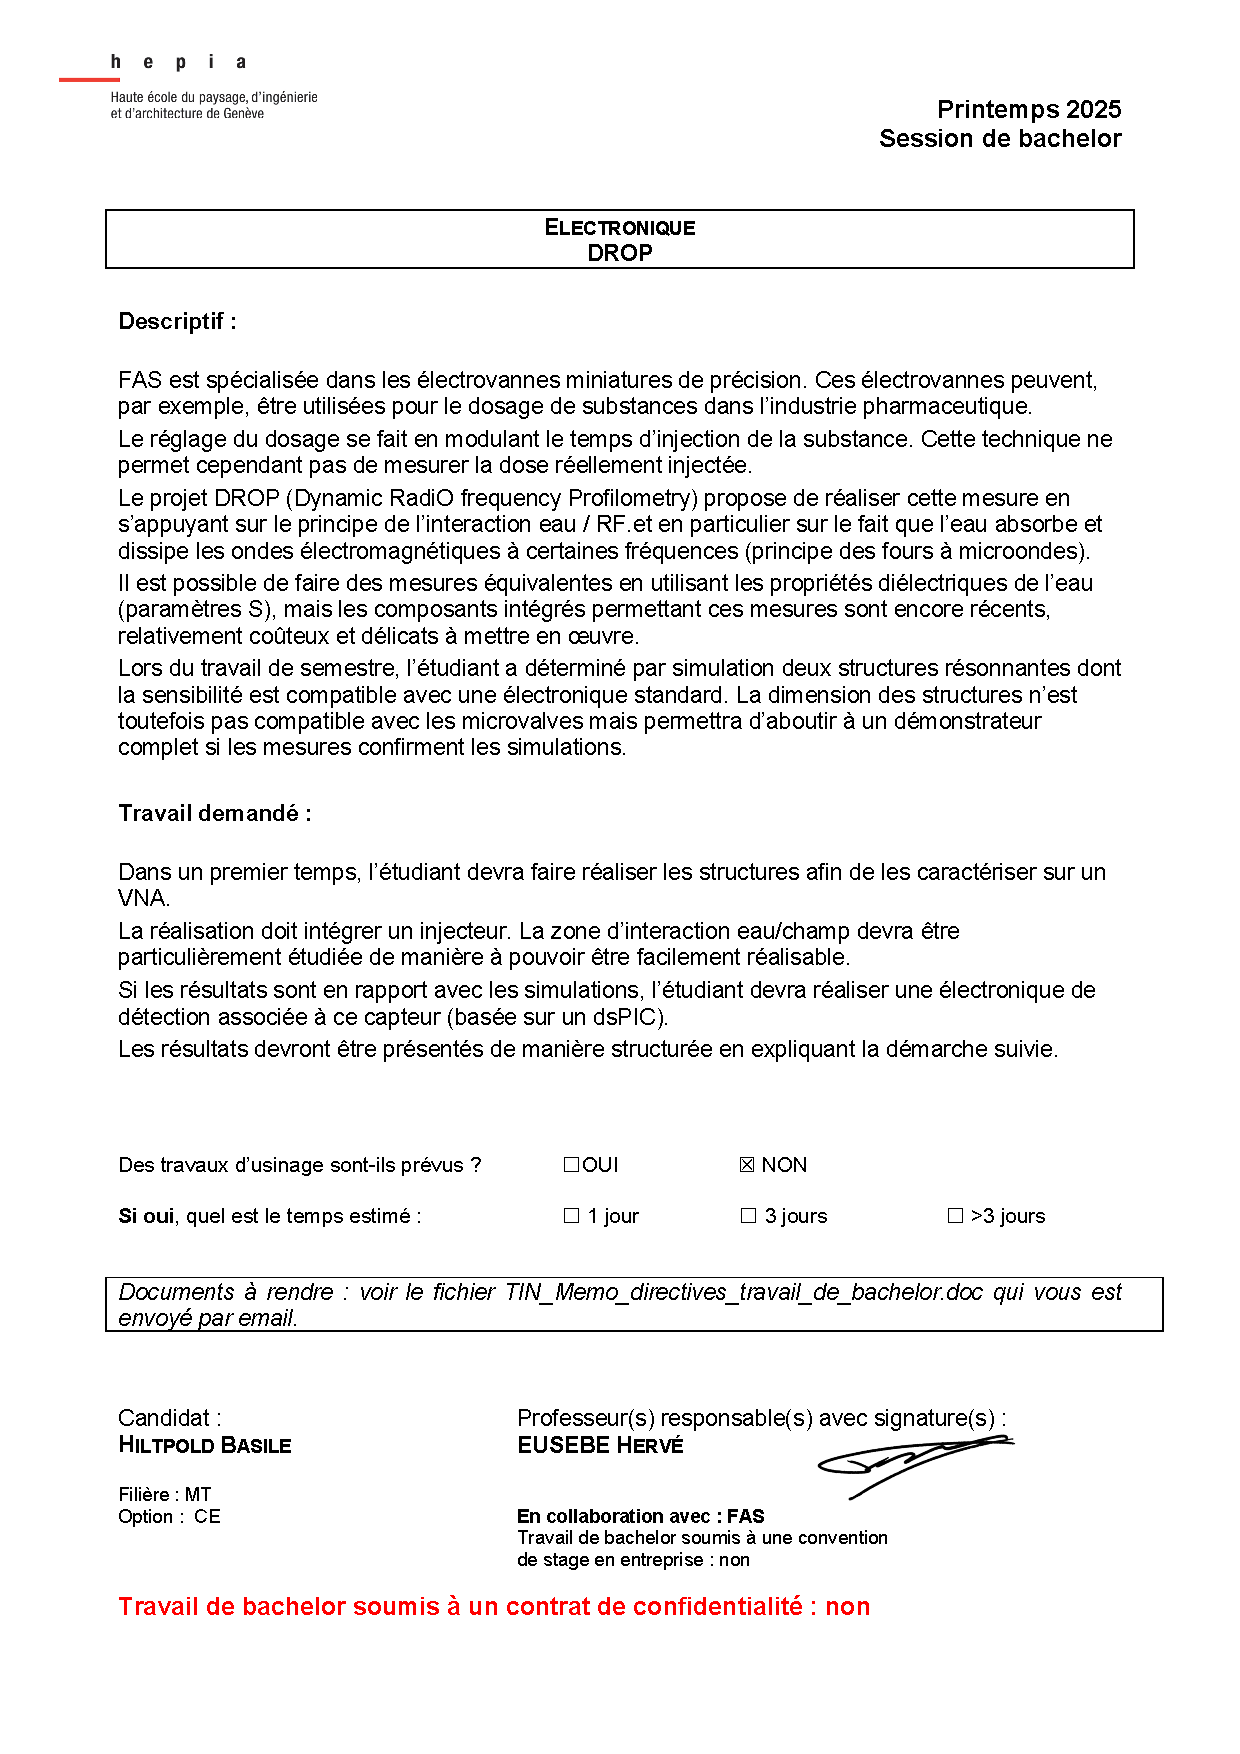
\includepdf{Enoncee.pdf}

\newpage
\vspace*{1cm}
{\huge \textbf{Résumé}}

\vspace{1cm}
L'industrie de la micro-fluidique, notamment dans le domaine de la pharmacologie, fait actuellement face à un problème de taille. En espérant trouver une solution, Fluid Automation Systems (FAS), une entreprise basée à Versoix spécialisée dans les électro-valves miniatures de précision, a misé sur ce travail de recherche.

\vspace{0.5cm}
L'objectif est de mettre au point un système de mesure de débit pour micro-fluide extrêmement précis. L'idée mise en œuvre pour réaliser cette mesure est d'utiliser les propriétés de l’électronique radiofréquence. En utilisant des filtres RF, un changement de milieu de propagation de l'onde induit une variation de la fréquence de coupure de ces derniers. 

\vspace{0.5cm}
Dans un second temps une électronique adaptée à un système embarqué a été mise en œuvre. Cette électronique sur mesure vise à remplacer l'analyseur de réseau vectoriel utilisé pour caractériser les capteurs durant la phase de conception. 

\vspace{1cm}
\begin{figure}[h]
    \centering
    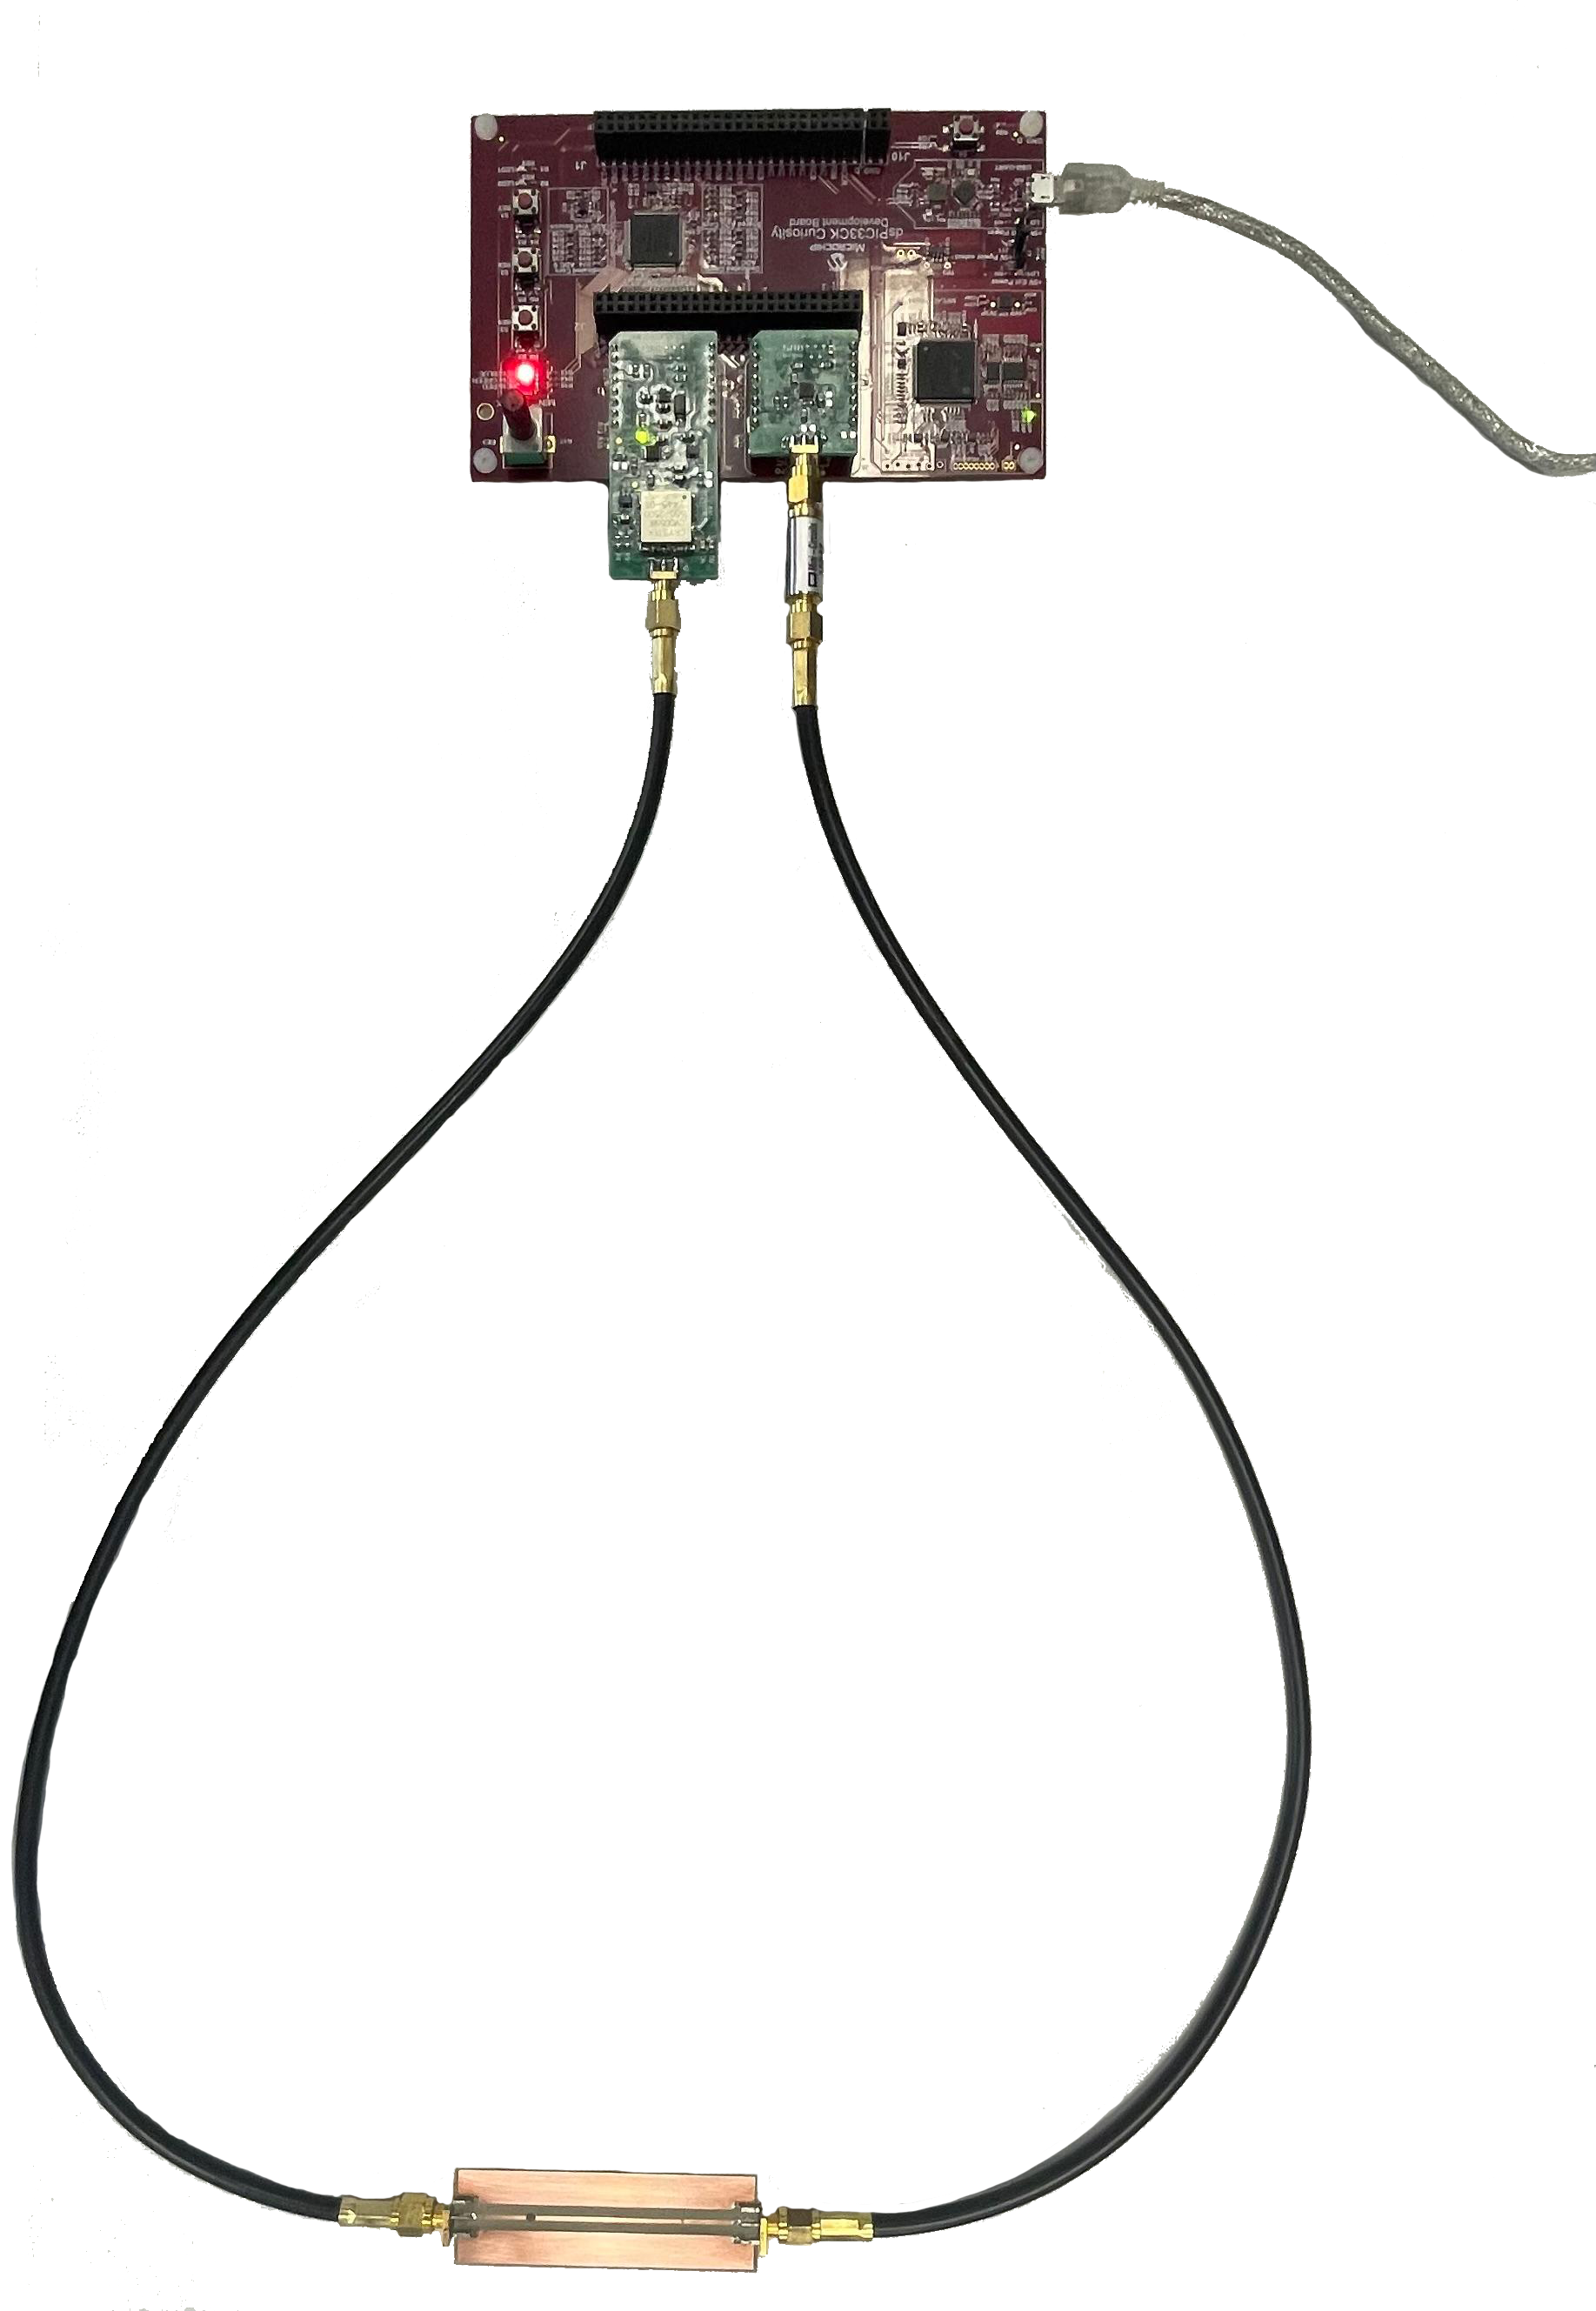
\includegraphics[scale=0.15, angle=90]{images/Systme.png}
\end{figure}

\newpage
\vspace*{1cm}
{\Large\textbf{Glossaire}}

\vspace{2cm}
\begin{tabular}{>{\bfseries}l @{\hspace{3cm}} l}
    FAS &  Fluid Automation Systems \\
    DROP &  Dynamic RadiO frequency Profilometry \\
    RF &  Radio fréquence \\
    VNA &  Vector Network Analyser \\
    VCO &  Voltage-controlled oscillator \\
    FR4 &  Flame Retardant 4 \\
    PCB &  Printed Circuit Board \\
    @STP &  at Standard temperature and pressure  \\
    ITU &  International Telecommunication Union  \\
    ISM &  Industrial, Scientific, and Medical  \\
    DC &  Direct Current  \\
    cc &  court-circuit  \\
    I2C &  Inter-Integrated Circuit  \\
    DAC &  Digital to Analog Converter  \\
    ADC &  Analog to Digital Converter  \\
  
\end{tabular}

\newpage
\vspace*{1cm}
\tableofcontents

\newpage
\vspace*{1cm}
\listoffigures

\newpage
\section{Introduction}
\subsection{Contexte}
Le projet DROP a vu le jour suite à une problématique soulevé par FAS, partenaire du projet. FAS est une entreprise Suisse basé à Versoix, spécialisés dans les systèmes micro-fluidiques et les micro-vannes. Elle fait partie depuis 2004 du groupe IMI Norgen ce qui lui a permis d’acquérir une envergure mondiale. Présent dans de nombreux secteurs tel que l'automobile, l'agroalimentaire, ferroviaire, énergétique, médical, et d'autres, FAS est une entreprise reconnue dans son domaine d'application. 

\vspace{0.5cm}
Le projet DROP existe pour résoudre une problématique liée aux micro-vannes utilisés dans la recherche pharmacologique et biologique. Il consiste à développer un appareil de mesure capable de mesurer des nano-volumes à grandes vitesse. Afin de ne pas perturber le fluide la mesure doit se faire sans contacte direct avec ce dernier. 

\vspace{0.5cm}
Les micro-vannes développée pas FAS, visible à la \textbf{figure~\ref{fig:uVanne}}, fonctionnent actuellement en boucle ouverte. Elles sont calibrées, avec des propriétés connues pour des fluides donné avec un signal de contrôle donné. Autrement dit, sans système de mesure, une moindre variation dans le  système peut induire une variation du volume injecté. Le projet DROP, en ajoutant cet organe de mesure, doit permettre d’améliorer grandement le système.

\vspace{0.5cm}
La \textbf{figure~\ref{fig:SchemauVanne}}, montre le fonctionnement des injecteurs. Le solénoïde responsable de l'ouverture de la vanne est piloté par un signal carré. Le temps haut du signal et la pression en amont définissent le volume des gouttes qui sortent de la vanne. Puisqu'elles fonctionnement en boucle ouverte, le volume des gouttes doit alors être mesuré à la conception dans des conditions connues supposé stable. Après avoir déterminé le volume d'une goûte le nombre voulu peut être injecter via le singal de commande. 

\vspace{0.5cm}
\begin{figure}[h]
    \centering
    \begin{subfigure}[b]{0.2\textwidth}
        \centering
        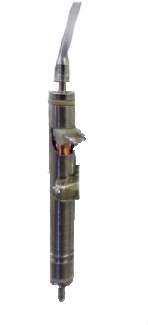
\includegraphics[scale=0.6]{images/FAS/uVanne.PNG}
        \caption{Micro-vanne}
        \label{fig:uVanne}
    \end{subfigure}
    \hfill
    \begin{subfigure}[b]{0.7\textwidth}
        \centering
        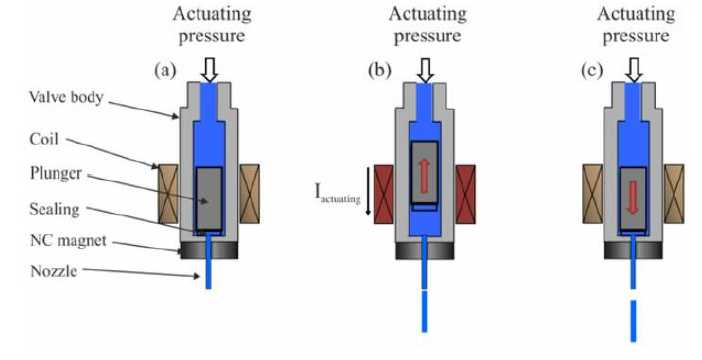
\includegraphics[scale=0.4]{images/FAS/uVanneSchema.png}
        \caption{Schéma micro-vanne}
        \label{fig:SchemauVanne}
    \end{subfigure}
    \vspace{0.5cm}
    \caption{Injecteurs FAS}
    \label{fig:Injecteurs_FAS}
\end{figure}

\newpage

Si le système DROP est mis en place l'approche devient différente. En effet, avec une mesure en sortie de l'injecteur, un système de régulation peut être mis en place. Un simple PID peut déjà s’avérer très efficace et le volume injecté serait garanti malgré de potentielles variations au sein du système.

\vspace{0.5cm}
\subsection{Solution envisagée}
Le système de mesure du projet DROP se base sur les propriétés de l'électronique RF. D'où le nom DROP pour Dynamic RadiO frequency Profilometry. En ef  fet, l'objectif consiste à détecter des gouttes, c'est-à-dire de petits volumes de fluide, qui, dans ce contexte, sont principalement constitués d'eau. Les propriétés de l'eau diffèrent de celles de l'air ainsi que du FR4 dans le domaine de la RF, et ce sont précisément ces différences qui seront exploitées pour la détection de l'eau.

\vspace{0.5cm}
Différentes structures RF ont été simulées avec Ansys HFSS, réalisées et caractérisées à l'aide VNA, afin de détecter une variation de fréquence de coupure et/ou de puissance en présence d'eau. 

\vspace{0.5cm}
Afin d’adapter cette méthode de mesure à un système embarqué, des cartes de développement compatibles avec mikroBus ont été conçues. Ces cartes fonctionnent par paires, une basée sur un VCO permet de générer un signal et l'autre permet de mesurer la puissance du signal qu'elle reçoit. Afin de piloter ces cartes, la  carte de développement dsPIC33CK Curiosity de chez Microchip a été utilisée.

\newpage
\section{Principes théoriques}
Les notions abordées dans ce chapitre sont évidentes, cependant un rappel de ces dernières semble tout à fait justifié. En effet, un tel rappel permet de consolider les bases théoriques indispensables au projet DROP.

\vspace{0.5cm}
\subsection{Les radiofréquences}
Les radiofréquences désignent une large plage de fréquences du spectre électromagnétique, allant jusqu’à 300 GHz. La limite inférieure définissant les radiofréquences n'est quant à elle pas clairement définie, elle dépend des normes, militaires ou civils, ou encore des régions d'applications. L'ITU commence à définir l'attribution des fréquences radio à partir de 8.3 kHz, dans l'édition 2024 du règlement des radiocommunications \textbf{[\ref{ref:radio_com}]}. Les radiofréquences se situent donc au début du spectre électromagnétique, dans les fréquences les plus basses, comme le montre  la \textbf{figure~\ref{fig:SpectreElectroMag}}.

\vspace{1cm}
\begin{figure}[h]
    \centering
    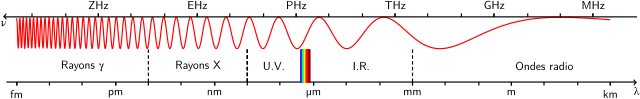
\includegraphics[scale=0.6]{images/Domaines_du_spectre_électromagnétique.svg.png}
    \caption{Domaine du spectre électromagnétique Par Benjamin ABEL}
    \label{fig:SpectreElectroMag}
\end{figure}

Au sein du projet DROP, ce sont les fréquences de la bande ISM 2.4 -2.5 Ghz qui sont en jeu pour les capteurs, à des fin de simplicité. Les bande ISM (Industrial, scientific, and medical) sont des plages de fréquences qui ont l'avantage de pouvoir être utilisées librement tant que les puissances sont respectées. Cependant certains tests ont été effectués en dehors de la bande ISM, donc la page intéressante du projet dans sa globalité est plutôt de 1 Ghz à 2.5 Ghz 

\subsection{Propriétés des matériaux en RF}
En RF, les matériaux ont des propriétés particulières intéressantes, notamment la permittivité relative, la célérité des ondes ou le coefficient de perte diélectrique.

\vspace{0.5cm}
La permittivité relative, généralement notée $\epsilon_r$, est une grandeur physique sans unité qui caractérise la capacité d'un matériau diélectrique à stocker de l’énergie électrique lorsqu'il est soumis à un champ électrique. La permittivité relative est définie comme le rapport entre la permittivité absolue du matériaux ($\epsilon$) et celle du vide ($\epsilon_0$). La permittivité relative est donnée par l'\textbf{équation \ref{eq:permittivité}}.

\newpage
\vspace{0.5cm}
{\Large
\begin{equation}
\epsilon_r = \frac{\epsilon}{\epsilon_0} 
\label{eq:permittivité}
\end{equation}}

\vspace{0.5cm}
Où: 

$\epsilon_0 \simeq 8.854 \cdot 10^{-12}$ F/m est la permittivité du vide.

$\epsilon$ en F/m est la permittivité absolue du matériau.

\vspace{0.5cm}
Une permittivité relative élevée indique que le matériau peut fortement polariser  ses charges internes en réponse à un champ électrique, ce qui augmente sa capacité à stocker de l’énergie électrostatique. La permittivité relative est essentielle car elle influence directement la propagation des champs électromagnétiques dans le matériau.

\vspace{0.5cm}
Dans le vide, $\epsilon_r = 1$, mais pour tout autre matériau, la permittivité relative est différente. Comme précisé dans le paragraphe précédent, la propagation des champs électromagnétique est directement influencée par la permittivité relative ce qui va donc avoir un impact sur la célérité des ondes dans le matériau donné. Cette célérité est donnée par l'\textbf{équation \ref{eq:celer}}.

\vspace{0.5cm}
{\Large
\begin{equation}
v = \frac{C}{\sqrt{\epsilon_r}} 
\label{eq:celer}
\end{equation}}

\vspace{0.5cm}
Où: 

$C \simeq 2.998 \cdot 10^8$ m/s est la vitesse de la lumière dans le vide. 

$\epsilon_r$ est la permittivité relative du matériau. 

\vspace{1cm}
Le coefficient de perte diélectrique, appelé aussi tangent de perte ou $tan\delta$ représente les pertes énergétiques dans le matériau lorsqu'il est soumis à un champ électrique variable. Le coefficient de perte diélectrique est défini comme étant le rapport entre la partie imaginaire et la partie réelle de la permittivité complexe du matériau. Le coefficient de perte diélectrique est donné par l'\textbf{équation \ref{eq:tand}}.

\vspace{0.5cm}
{\Large
\begin{equation}
\tan\delta = \frac{\epsilon''}{\epsilon'} 
\label{eq:tand}
\end{equation}}

\vspace{0.5cm}
Où: 

$\epsilon'$ est la partie réelle de la permittivité liée au stockage d’énergie. 

$\epsilon''$ est la partie imaginaire de la permittivité liée à la dissipation d’énergie (généralement sous forme de chaleur). 

\vspace{0.5cm}
Un faible $\tan\delta$ indique un matériau faiblement dissipatif (quasi-idéal), tandis qu’un $\tan\delta$ élevé indique un matériau dans lequel les pertes diélectriques sont significatives. C'est un paramètre important puisque il est directement liée aux pertes dans un système RF.

\vspace{0.5cm}
Dans le cadre du projet DROP, 3 matériaux sont particulièrement intéressant. Dans un premier temps le FR4, puisqu'il sera le substrat utilisé pour les différents circuits. Ensuite, il y a les propriétés de l'air et de l'eau. En effet, les fluides injectés étant principalement aqueux, et afin de simplifier l'étude, les propriétés de l'eau sont suffisamment proches de celles des fluides cibles.

\vspace{1cm}
\subsubsection{FR4}
Le FR4 est un matériau composite de résine époxyde incluant de la fibre de verre. Ce dernier est grandement utilisé dans le domaine de l’électronique et en majeur partie lors de la fabrication de PCB. Il a l'avantage de ne pas être inflammable, ce qui en fait un matériau sûr pour éviter le déclenchement d'incendie en cas de dysfonctionnement du circuit. Au sein du projet, les circuits imprimés ont tous été réalisés avec du FR4 comme substrat.

\vspace{1cm}
{\large\textbf{Caractéristiques:}}
\vspace{0.5cm} \\
\textbf{Permittivité relative:} \\
$\epsilon_r = 3.9 \to 4.7$
\vspace{0.5cm}\\
\textbf{Vitesse de propagation:} \\
$v = 1.384 \to 1.519 \cdot 10^8$ m/s
\vspace{0.5cm}\\
\textbf{Coefficient de perte diélectrique:}\\
$\tan\delta = 0.02 \to 0.03$ 
\vspace{1cm}

Il est important de noter que ces valeurs sont des plages relativement larges. Ces paramètres dépendent de plusieurs facteurs allant de la fabrication du FR4 en lui même à la fréquence des signaux qui le traverseront. Lors de ce travail les valeurs utilisées pour les calculs et les simulations seront une permittivité $\epsilon_r = 4.4$, Une vitesse de propagation $v=1.43 \cdot 10^8$ et un coefficient de perte $\tan\delta=0.02$. Ces valeurs restent des choix arbitraires puisque le FR4 ne garantit pas ces caractéristiques pour la RF, les vendeurs les plus pessimistes conseillent de changer de matériaux à partir de 2 Ghz.

\newpage
\subsubsection{Air}
La définition du mot air peut parfois faire débat, afin de clarifier les choses l'air dont il s'agit dans ce document n'est autre que celle de l’atmosphère définie comme étant de l'air sec composé à 78.08 \% de diazote, 20.95\% de dioxygène et moins de 1\% de gaz rares. Cet air étant à une pression de 1 bar.

\vspace{1cm}
{\large\textbf{Caractéristiques:}}
\vspace{0.5cm} \\
\textbf{Permittivité relative:} \\
$\epsilon_r = 1.00058986 \pm 0.00000050 @STP$ 
\vspace{0.5cm}\\
\textbf{Vitesse de propagation:} \\
$v \simeq C \simeq 2.998 \cdot 10^8$ m/s
\vspace{0.5cm}\\
\textbf{Coefficient de perte diélectrique:}\\
$\tan\delta \simeq 0$ 
\vspace{1cm}

Les Caractéristiques de l'air en RF sont très similaires à celles du vide. Ces caractéristiques sont influencées par une infinité de paramètres, allant de la répartition des gaz qui composent l'air, à la pression, en passant par la température. Mais ces derniers ont un impact infime, négligeable dans la majorité des cas. Ces caractéristiques sont données pour de l'air sec, cependant, la majorité du temps, l'air que l'on retrouve dans l'atmosphère au niveau du sol est humide, avec un taux d'humidité relative variable. Les données de MeteoSwiss indiquent une humidité relative sur les 12 derniers mois variant entre 40\% et 100\%.  

\vspace{0.5cm}
Pour comprendre l'impact de l'humidité de l'air sur les caractéristiques de l'air en RF, il faut, dans un premier temps, comprendre la différence entre l'humidité absolue et relative. Un article mis en ligne par l'office fédéral de météorologie et de climatologie \textbf{[\ref{ref:air_hum}]} sur le site de la confédération Suisse explique les principes de l'humidité de l'air. Ce dernier précise que l'humidité absolue désigne la quantité de vapeur d'eau contenue dans l'air en $g/m^3$. Elle reflète la quantité réelle d'eau qui se trouve dans l'air. L'humidité relative, quant à elle, représente la proportion de vapeur d'eau contenue dans l'air par rapport à la capacité maximale de vapeur d'eau que peut contenir l'air. Une humidité relative de 100\% signifie que l'air est saturé en vapeur d'eau et cette dernière va se condenser, former des gouttelettes qui elles sont bien à l'état liquide et forment du brouillard ou des nuages. Malgré une humidité relative de 100\%, la vapeur d'eau ne dépasse généralement pas 5\% du volume total de l'air.

\vspace{0.5cm}
Le fait, que l'influence de l'humidité de l'air sur ses caractéristiques en RF soit négligeable, est due à 2 raisons principales. Premièrement, une humidité de 100\%  ne représente en réalité qu'un faible volume de vapeur d'eau. Deuxièmement, les caractéristiques RF de l'eau à l'état gazeuse sont très proches de celles de l'air, puisque dans cet état les molécules d'eau sont éloignées et n'interagissent que très peu entre elles, l'ensemble n'est que peu polarisable par un champ électrique. Dans le cas contraire, si l'eau commence à se condenser, il risque d'y avoir des effets de rosé. Se retrouver avec de l'eau à l'état liquide sur les PCB poserait d'autres problèmes que ceux liés à l'humidité de l'air en tant que tel. 

\vspace{0.5cm}
Pour des cas plus particulié, le document \textbf{[\ref{ref:air_storm}]} traite de la variation de certaines caractéristiques, notamment lors de tempête de sable ou de poussière avec de l'air emprisonné dans des échantillons poreux. 

\subsubsection{Eau}
Les propriété RF de l'eau sont très sensibles à la température mais aussi à la fréquence des ondes qui la traverse. Comme pour l'air, il est nécessaire de définir l'eau, au sein du projet DROP l'eau fait référence à de l'eau du robinet à 20°C. Les informations qui suivent sont issues de l'article \textbf{[\ref{ref:water_prop}]}. On y retrouve notamment la \textbf{figure~\ref{fig:WaterPropImg}}. Elle démontre la variation de la permittivité et du facteur de perte de l'eau en fonction de la fréquence et de la température. 

\vspace{1cm}
\begin{figure}[h]
    \centering
    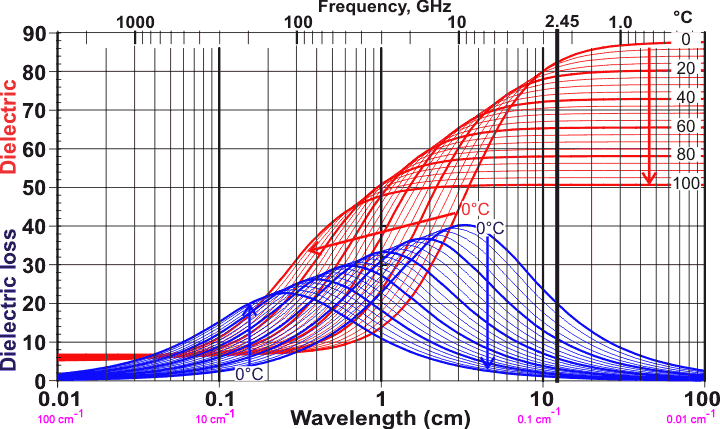
\includegraphics[scale=0.5]{images/WaterPropImage.png}
    \caption{Permittivité et facteur de perte de l'eau entre 0 °C et 100 °C}
    \label{fig:WaterPropImg}
\end{figure}

Les paramètres retenus pour l'eau pour les simulations et calculs sont ceux à 20°C à 1 Ghz, soit les caractéristiques ci-dessous. Une augmentation de la fréquence jusqu’à 2.5 GHz induira une diminution de la permittivité et une augmentation des pertes, mais cette variation est négligeable par rapport aux caractéristiques l'air ou au FR4. 

\newpage
\vspace{1cm}
 {\large\textbf{Caractéristiques:}}
\vspace{0.5cm} \\
\textbf{Permittivité relative:} \\
$\epsilon_r = 80$ 
\vspace{0.5cm}\\
\textbf{Vitesse de propagation:} \\
$v \simeq 3.354 \cdot 10^7$ m/s
\vspace{0.5cm}\\
\textbf{Coefficient de perte diélectrique:}\\
$\tan\delta \simeq 1$ 
\vspace{1cm}

\subsection{L’électronique RF}
En électronique, tout signal quel qu'il soit est en réalité une onde électromagnétique. Cela peut paraître contre intuitif car en électronique dite classique les équations de Maxwell sont grandement simplifiées. En effet, même une alimentation DC au sein d'un PCB, à l'instant ou ce dernier est mis sous tension, l'alimentation va générer une onde électromagnétique, voyageant entre les pistes de l'alimentation et la masse, ces dernières formant un guide d'onde. Une fois l'alimentation établie, il n'est plus question d'onde, mais le champ électrique est constant, et le champ magnétique se situe autour des pistes suite au passage du courant. 

\vspace{0.5cm}
Une seconde notion importante souvent faussement établie est le transfert d’énergie. C'est une notion encore une fois contre intuitive mais le transfert d'énergie n'est pas dû au passage des électrons dans le conducteur ou la charge. Dans un conducteur, pour des courants alternatifs, les électrons ont une vitesse moyenne nulle sur une période, tandis que pour un courant continu, la vitesse des électrons dans le conducteur est appelée vitesse de dérive des électrons. Cette vitesse est donnée par l'\textbf{équation \ref{eq:electron_speed}}.

\vspace{0.5cm}
{\large
\begin{equation}
v_d = \mu E 
\label{eq:electron_speed}
\end{equation}}

Où:

$v_d$ = vitesse de dérive en $m/s$

$\mu$ = mobilité de l'électron dans le matériaux en $m^2/V\cdot s$

$E$ = champ électrique en $V/m$

\newpage
On constate que la vitesse de dérive est proportionnellement liée au champ électrique. Le cuivre a une mobilité de l'électron comprise entre $3 \cdot10^-3$ à $5\cdot10^-3 \space m^2/V\cdot s$. Cette mobilité dépend notamment de la température ou de la pureté du cuivre. Sur un fil de cuivre de 1 m de longueur avec une chute de tension de 1 V, ce qui est énorme dans beaucoup de cas, n'induit un champ électrique que de $1 V/m$. On a donc dans ce cas une vitesse de dérive des électrons comprise entre $3$ et $5 \space mm/s$. Ce qui est très lent à l'échelle de l'électronique. 

\begin{comment}
\vspace{0.5cm}
Si une résistance est branchée en série sur le circuit, le courant qui la traverse doit être le même que dans les fils, dans la majorité des cas, toute la tension se retrouve sur la résistance, elle a un donc un champ électrique beaucoup plus important que celui dans les fils. Ce qui résulte en une vitesse de dérive des électron beaucoup plus élevé dans la résistance. Et cela est très facile à s’imager avec la \textbf{figure~\ref{fig:UIR}}, qui est une illustration de la loi d'ohm très connue. La résistance peut être imaginée comme un "rétrécissement" du conducteur, et le flux d'électron doit être le même de part et d'autre de cette résistance, pour ce faire la vitesse de dérive des électron doit être plus élevée dans ce "rétrécissement".

\vspace{1cm}
\begin{figure}[h]
    \centering
    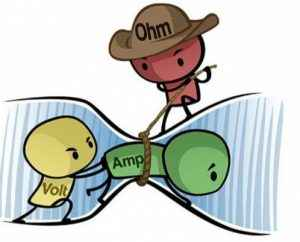
\includegraphics[scale=0.4]{images/Cartoon-Volt-Amp-Ohm.jpg}
    \caption{Illustration du lien entre tension courant et résistance.}
    \label{fig:UIR}
\end{figure}
\end{comment}

\vspace{0.5cm}
Le véritable flux d'énergie est donné par le vecteur Poynting. Le vecteur Poynting, donné dans l'\textbf{équation \ref{eq:poynting_vector}}, est simplement le produit vectoriel du champ électrique et magnétique multiplié par une constante.

\vspace{0.5cm}
{\large
\begin{equation}
S = \frac{1}{\mu_0} E\times B
\label{eq:poynting_vector}
\end{equation}}

(Dans le vide)

Où:

$S$ est le vecteur Poynting

$\mu_0$ est la perméabilité magnétique du vide

$E$ est le vecteur du champ électrique

$B$ est le vecteur du champ magnétique 

\vspace{0.5cm}
Par définition, le vecteur Poynting correspond à la densité de flux liée à la propagation de l'onde électromagnétique. Ce flux, à travers une surface fermée ou non, équivaut à la puissance transmise par l'onde dans cette surface. Bien qu'il définisse le flux pour la propagation des ondes, il fonctionne aussi en mode stationnaire. Le premier exemple, à la \textbf{figure~\ref{fig:coax_poynting}}, représente un câble coaxial traversé par un courant. On y retrouve en rouge le champ électrique, en bleu le champ magnétique induit par le courant, et en vert le vecteur Poynting qui est en tout point le produit vectoriel du champ électrique et magnétique.

\vspace{1cm}
\begin{figure}[h]
    \centering
    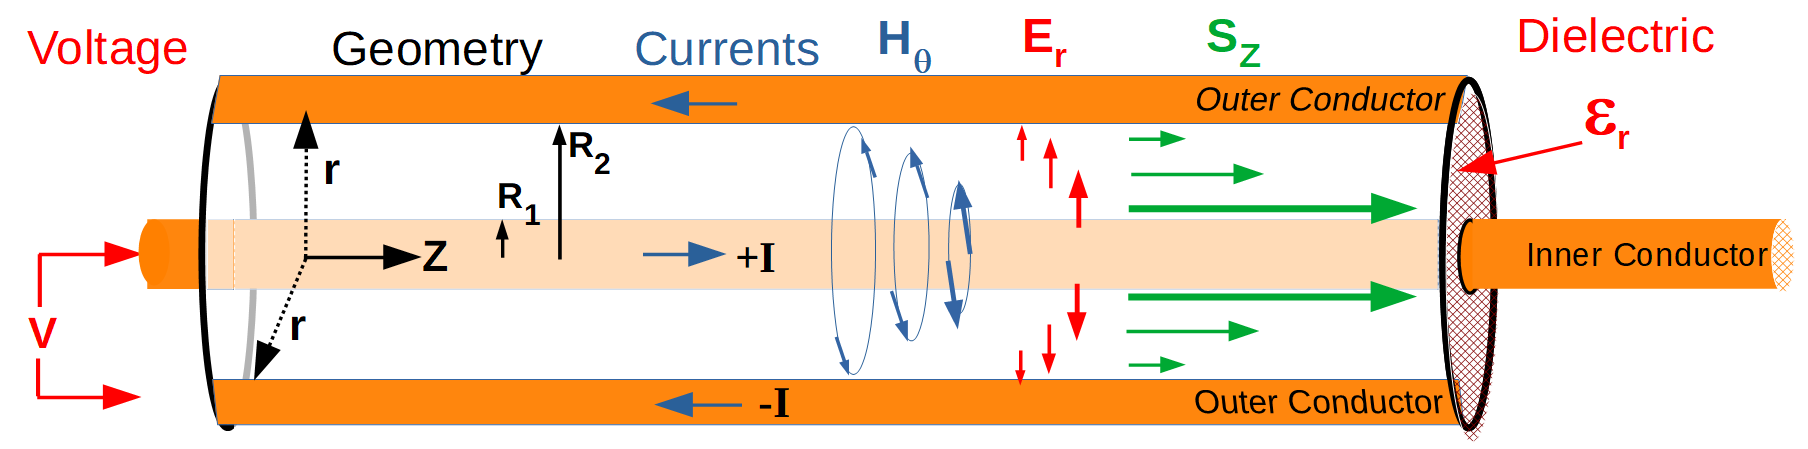
\includegraphics[scale=0.2]{images/CoaxPoyntingVector.png}
    \caption{Illustration du flux d'énergie dans un câble coaxial.}
    \label{fig:coax_poynting}
\end{figure}

\newpage
L'énergie véhiculée par ce signal électrique quel qu'il soit passe dans tous les cas par le diélectrique du câble du coaxial.

\vspace{0.5cm}
Dans le cas d'un circuit DC basique comprenant simplement une batterie et une lampe, l'énergie est transmise dans l'air entre les conducteurs, et non dans les conducteurs en eux mêmes. Ceci est représenté dans la \textbf{figure~\ref{fig:dc_poynting}}.

\vspace{1cm}
\begin{figure}[h]
    \centering
    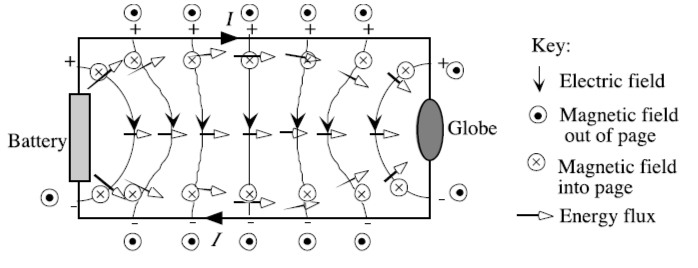
\includegraphics[scale=0.6]{images/poynting_dc.png}
    \caption{Illustration du flux d'énergie dans un circuit DC.}
    \label{fig:dc_poynting}
\end{figure}

Pour le cas des signaux alternatifs, cette notion est encore plus simple, en effet le courant faisant des va et vient et les électrons ayant donc une vitesse moyenne nulle, il était clair que l'énergie ne circulait pas grâce à ces derniers. Le principe est exactement le même que pour les circuit DC, le champ électrique change de sens au même moment que le courant. Le champ magnétique change donc aussi de sens, le vecteur Poynting étant le produit vectoriel de ces 2 composantes, si les 2 changent de direction, le vecteur Poynting lui reste inchangé et pointe continuellement de la source vers la charge.

\vspace{0.5cm}
Ces notions de l'électronique sont certes plus fidèles à la réalité mais plus complexes à mettre en œuvre, que ce soit de voir chaque signaux comme des ondes ou alors d'utiliser Poynting pour le transfert d'énergie. Dans la majorité des cas pour les circuits DC ou alors de faible fréquence, beaucoup de notions sont simplifiées et cela fonctionne très bien. Cependant, pour que cela fonctionne, il faut que les dimensions du circuit soient 10 à 20 fois inférieures à la longueur d'onde mis en jeu. Dans le cas du projet DROP la plage de fréquence de 1 Ghz à 2.5 GHz donne des longueurs d'onde allant de 57.2 mm à 143 mm dans du FR4. Ces valeurs sont calculées grâce aux \textbf{équations \ref{eq:lambda_vitesse}}. Ces dimensions imposent donc une réflexion plus poussée que l'électronique basique, on parlera donc d'électronique RF. 

\vspace{0.5cm}
{\large
\begin{equation}
\lambda = \frac{v}{f} \hspace{3cm} v = \frac{c}{\sqrt{\varepsilon_r}}
\label{eq:lambda_vitesse}
\end{equation}}
\vspace{1cm}

\newpage
\subsubsection{VNA}
Le VNA, ou analyseur de réseau vectoriel, est un outil de mesure indispensable pour faire de l'électronique RF. En mesurant la transmission et la réflexion sur chacun de ces 4 ports l'analyseur de réseau permet de caractériser une multitude de réseaux RF, tels que des filtres, des lignes de transmissions, des antennes etc.

\vspace{0.5cm}
Le VNA mesure la réponse en fréquence des réseaux qui lui sont présentés, en amplitude et en phase. Ces mesures permettent de connaître les paramètres S de nos réseaux en fonction de la fréquence. Celui utilisé pour ce travail est un Agilent E5071C, il permet des mesures allant de 9 kHz jusqu’à 8.5 GHz.

\newpage
\subsection{Guide d'onde et structure RF}
Les fréquences utilisées pour le projet DROP étant relativement élevées, cela implique des longueurs d'onde assez courtes pour qu'il soit nécessaire de réfléchir autrement que pour de l'électronique dite classique.

\vspace{0.5cm}
En première partie, cette section abordera 2 types de guides d'ondes très communs en électronique RF, les lignes microruban et coplanaire. Entre autre, le comportement du champ électrique et magnétique pour ce genre de ligne, la propagation de l'onde et sa célérité.  

\vspace{0.5cm}
En seconde partie, cette section sera consacrée à deux structures RF. Elle explique premièrement le fonctionnement des Stub, qui sont un incontournable autant pour ligne microruban que coplanaire et tout autre guide d'onde. La deuxième structure détaillée est un résonateur demi onde série sur ligne microruban et coplanaire.

\vspace{1cm}
\subsubsection{Ligne microruban}
Les formules citées ci-dessous dans ce paragraphe sur les lignes microruban proviennent de l'ouvrage \textbf{[\ref{ref:Microstrip_line_theor}]}.

\vspace{0.5cm}
Les lignes microruban, ou micrstrip line en anglais, sont des lignes de transmission faciles à mettre en œuvre sur PCB. Elles permettent de transporter les signaux RF au sein d'une carte tout en contrôlant l’impédance de ces dernières.

\vspace{0.5cm}
La \textbf{figure \ref{fig:microruban_champ}} est une vue en coupe d'une ligne microruban. On y voit en jaune la piste de cuivre, juste en dessous le substrat et un plan de masse à l'opposé. 

\begin{figure}[h]
    \centering
    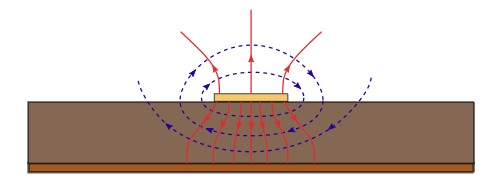
\includegraphics[scale=0.7]{images/microruban_champ.png}
    \caption{Ligne microruban en coupe}
    \label{fig:microruban_champ}
\end{figure}

On y voit aussi en rouge les ligne du champ électrique et en bleu celles du champ magnétique. Le champ électrique va de la ligne vers la masse, bien qu'il soit aussi présent dans l'air, c'est dans le substrat qu'il est le plus intense. Quant au champ magnétique, il est quasiment perpendiculaire au champ électrique en tout point de ce dernier ce qui rend la ligne microruban proche du mode TEM. 

\newpage
\vspace{0.5cm}
Une ligne ruban dans un diélectrique entre 2 plans de masses, avec un PCB 3 couche par exemple, est quant à elle TEM. Cependant, elle est bien moins pratique que la ligne microruban classique, puisque c'est une couche interne, aucun composant peut y être directement soudé et doit passer par des via.

\vspace{0.5cm}
Le champ électromagnétique étant principalement dans le substrat, c'est aussi dans ce dernier que les ondes vont s'y déplacer principalement. Afin de connaître la célérité des ondes dans une ligne microruban, il faut connaître la permittivité effective de la structure, cette dernière peut être approximé avec l'\textbf{équation \ref{eq:eps_eff}}.

\vspace{0.5cm}
{\large
\begin{equation}
\epsilon_{eff} = \frac{\epsilon_r+1}{2} + \frac{\epsilon_r-1}{2}q 
\label{eq:eps_eff}
\end{equation}}

\vspace{0.5cm}
{\large
\begin{equation}
q = \frac{1}{\sqrt{1+12(h/w)}}+q2 
\label{eq:q}
\end{equation}}

\vspace{0.5cm}
{\large
\begin{equation}
q2 = \left\{
\begin{array}{ll}
  0.04(1-\frac{w}{h})^2, & \text{si} \hspace{0.3cm}\frac{w}{h}\leq 1 \\
  0, & \text{si} \hspace{0.3cm}\frac{w}{h}\geq 1
\end{array}
\right.
\label{eq:q2}
\end{equation}}
\vspace{1cm}

Avec : \\
$\epsilon_r$ la permittivité du substrat\\
$h$ la hauteur du substrat\\
$w$ la largeur de la piste

\vspace{1cm}
Sans entrer dans le détail des calculs, la courbe de la \textbf{figure \ref{fig:microperm}} en annexe donne la permittivité effective d'une ligne microruban en fonction de la largeur de la piste avec les propriétés des PCB utilisées dans ce travail. C'est à dire une épaisseur du substrat de 1.6 mm avec une permittivité relative $\epsilon_r=4.4$. La permittivité effective augmente avec la largeur. En effet, plus la piste est large plus le champ est concentré dans le substrat et inversement. Ainsi, plus le champ est concentré dans le substrat plus la permittivité effective se rapproche de celle du substrat.

\newpage
\vspace{0.5cm}
La vitesse de propagation des ondes dans la ligne microruban peut donc être calculée avec l'\textbf{équation \ref{eq:celer}} en utilisant la permittivité effective. La courbe de la \textbf{figure \ref{fig:microceler}} en annexe présente la célérité de l'onde en fonction de la largeur de piste dans les mêmes conditions que pour les calculs de la permittivité effective. La vitesse varie de 0.61 à 0.52 fois la vitesse de la lumière. C'est bon à savoir mais cela ne pose pas de problème dans la majorité des cas. Premièrement car, pour une avoir impédance adaptée au sein du même circuit, les lignes feront toutes la même largeur. Deuxièmement car, avec une ligne extrêmement fine tendant vers 0 et une ligne de 10 mm de largeur, 1 m de longueur de ligne induit un retard d'environ 1 ns. Les détails du calcul se trouvent à l'\textbf{équation \ref{eq:timediffmicro}} en annexe.

\vspace{0.5cm}
Dernier point important pour la ligne microruban est son impédance. En effet, afin de garantir un transmission maximal du signal le long de la ligne, il est important que tous les éléments de la source à la charge soient adaptés en impédance. Le VNA et autre composant classique de la RF étant tous adaptés à 50 ohm, c'est naturellement à 50 ohm que les lignes sont généralement adaptées. L’impédance d'une ligne microruban est donné par l'\textbf{équation \ref{eq:microz}}.

\vspace{0.5cm}
{\Large
\begin{equation}
Z_{microruban} = \left\{
\begin{array}{ll}
  \frac{Z_0}{2\pi\sqrt{\epsilon_{eff}}}ln(8\frac{h}{w}+\frac{w}{4h}), & \text{si} \hspace{0.3cm}\frac{w}{h}\leq 1\\
  \frac{Z_0}{\sqrt{\epsilon_{eff}[\frac{w}{h}+1.393+0.667ln(\frac{w}{h})+1.444]}}, & \text{si} \hspace{0.3cm}\frac{w}{h}\geq 1
\end{array}
\right.
\label{eq:microz}
\end{equation}}

\vspace{0.5cm}
Où: \\
$Z_0 \simeq 376.73 \hspace{0.2cm}\Omega$ est l’impédance de l'espace libre

\vspace{1cm}
Comme pour la permittivité effective et la célérité, la \textbf{figure \ref{fig:microimped}} en annexe montre l’impédance de la ligne en fonction de la largeur de la piste pour les même paramètres de PCB.

\vspace{0.5cm}
Le logiciel Qucs, utilisé dans ce travail, possède des outils de calculs de ligne qui ont permis la vérification des calculs et des courbes. Pour une ligne adaptée à $50\Omega$, la \textbf{figure \ref{fig:microimped}} donne une ligne de largeur 3 mm environ. La table de calcul donne pour cette largeur $50.79\Omega$. Qucs quant à lui donne, pour une largeur de 3 mm et les mêmes paramètres du substrat, $50.56\Omega$ d’impédance et un $\epsilon_{eff}$ de $3.34$.  

\newpage
\subsubsection{Ligne coplanaire}
Les lignes coplanaire ou CPW (Coplanar Waveguide) en anglais, sont des lignes de transmission qui sont, comme le microruban, faciles à mettre en œuvre sur PCB. Elles permettent aussi d'avoir une impédance contrôlée, mais contrairement à la ligne microruban, d'autres paramètres que la largeur de la ligne sont contrôlables. 

\vspace{0.5cm}
La \textbf{figure \ref{fig:CPW_Coupe}} est une vue en coup d'une ligne coplanaire. On y retrouve une ligne centrale, entourée par la masse à gauche et à droite de cette dernière, le tout sur un substrat.

\vspace{1cm}
\begin{figure}[h]
    \centering
    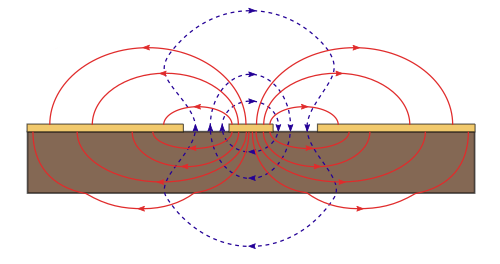
\includegraphics[scale=0.7]{images/coplanair_champ.png}
    \caption{Ligne coplanaire en coupe}
    \label{fig:CPW_Coupe}
\end{figure}

Comme pour la ligne microruban, on retrouve sur l'image les champs électriques en rouge et les champs magnétiques en bleu. Le champ électrique allant toujours de la ligne vers la masse, mais cette fois ci en passant tout autant par l'air que par le substrat. C'est aussi une ligne qui présente un mode de propagation proche du mode TEM.

\vspace{0.5cm}
Dans le cas de la ligne coplanaire, en plus de la largeur de la piste, il y a le gap entre la piste et les zones de masse qui entre en compte. Les paramètres du PCB restent les mêmes que pour la ligne microruban, une hauteur de substrat de 1.6 mm avec une permittivité de 4.4, pour les calculs qui suivent.

\newpage
\vspace{0.5cm}
Les équations suivantes sont issues du livre \textbf{[\ref{ref:MicroWaveRfDesign}]}. L'\textbf{équation \ref{eq:cpwperm}} permet de calculer la permittivité effective d'une ligne coplanaire.

\vspace{0.5cm}
{\large
\begin{align}
\epsilon_{eff} =\; & 0.5\left(\epsilon_r+1\right)
\left(\tanh\left(1.785\log\left(\frac{h}{s}\right)+1.75\right)\right. \nonumber \\
& \left. + \left(\frac{ks}{h}\right)
\left(0.04-0.7k+0.01\left(1-0.1\epsilon_r\right)\left(0.25+k\right)\right)\right)
\label{eq:cpwperm}
\end{align}
\vspace{1cm}
}


Où:\\
$\epsilon_r$ est la permittivité du substrat\\
$h = 1.6$ mm est la hauteur du substrat\\
$s$ est le gap entre la ligne et la masse\\
$k$ est donné dans l'\textbf{équation \ref{eq:cpwk}}

\vspace{0.5cm}
{\large
\begin{equation}
k=\frac{w}{w+2s}
\label{eq:cpwk}
\end{equation}
\vspace{1cm}
}

Où:\\
$w$ est la largeur de la piste

\vspace{1cm}
La permittivité effective, par rapport à la largeur de piste et pour différents gap, se trouve dans la \textbf{figure \ref{fig:cpwperm}} en annexe. On peut voir que la permittivité effective diminue lorsque la largeur de la piste augmente mais diminue aussi lorsque le gap augmente. 

\vspace{0.5cm}
Quand à la célérité de l'onde, elle se trouve dans la \textbf{figure \ref{fig:cpwceler}} en annexe. Contrairement à la ligne microruban elle augmente lorsque la largeur de la piste augmente, ce qui est le résultat attendu puisque elle est directement liée à la permittivité effective.  

\newpage
Quant à l’impédance d'une ligne coplanaire, elle est calculée avec l'\textbf{équation \ref{eq:cpwimped}}. Cependant $K(k)$ est une intégrale elliptique complète du premier genre, pour simplifier les calculs, une approximation commune en électronique RF basée sur les travaux de Abramowitz et Stegun a été utilisée, elle est présentée dans l'\textbf{équation \ref{eq:Ksimpli}} ou \textbf{\ref{eq:Ksimpli2}}.

\vspace{0.5cm}
{\large
\begin{equation}
Z_0=\frac{30\pi}{\sqrt{\epsilon_{eff}}}\frac{K'(k)}{K(k)}
\label{eq:cpwimped}
\end{equation}
\vspace{1cm}
}

Où :
{\large
\begin{equation}
k'=\sqrt{(1-k^2)}
\hspace{1cm}
\text{et}
\hspace{1cm}
K'(k)=K(k')
\label{eq:cpwk'}
\end{equation}
\vspace{1cm}
}

{\large
\begin{equation}
\frac{K(k)}{K'(k)} \approx \frac{1}{\pi}\ln\left(
2\frac{1+\sqrt{k}}{1-\sqrt{k}}
\right) \hspace{2cm} 0\leq k\leq0.707
\label{eq:Ksimpli}
\end{equation}
}

\vspace{0.5cm}
{\large
\begin{equation}
\frac{K'(k)}{K(k)} \approx \frac{1}{\pi}\ln\left(
2\frac{1+\sqrt{k'}}{1-\sqrt{k'}}
\right) \hspace{2cm} 0.707\leq k\leq1
\label{eq:Ksimpli2}
\end{equation}
\vspace{1cm}
}

\vspace{0.5cm}
Les courbes d’impédance en fonction de la largeur de piste et du gap se trouvent à la \textbf{figure \ref{fig:cpwimped}} en annexe. Il est possible d'y constater que passé une certaine largeur, l'influence sur l’impédance est presque nulle et seul le gap peut impacter l'impédance. 

\vspace{0.5cm}
Qucs et HFSS ne font pas ces approximations, Qucs car il résout les intégrales elliptiques, et HFSS car il calcule directement la réponse du système avec les équations de maxwell. Ils possèdent donc des résultats plus précis et plus juste que ceux présents en annexe.
Si par exemple, je souhaite adapter mon impédance avec un gap de 0.2 mm, en utilisant le calculateur de ligne de Qucs il me faut une piste de 1.7 mm de large, ce qui me donne une impédance de $49.99 \Omega$. Cela correspond plus ou moins avec mes calculs qui me donne, pour les mêmes paramètres, une impédance de $51\Omega$. 

\newpage
\subsubsection{Stub}
Dans le domaine des radiofréquences, un stub est une section de ligne de transmission ou de guide d'onde connecté au circuit à une seul extrémité. L'autre extrémité, au niveau de la partie libre du stub, peut être soit ouvert, soit en court-circuit. En négligeant les perte dans la ligne, l'impédance d’entrée du stub est purement réactif, soit capacitif soit inductif, dépendamment de sa longueur, du type de terminaison ou de la fréquence.

\vspace{1cm}
\begin{figure}[h]
    \centering
    \begin{minipage}[b]{0.445\textwidth}
        \centering
        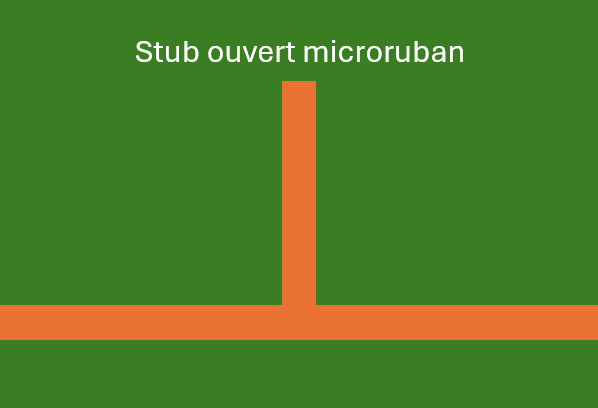
\includegraphics[width=\textwidth]{images/microstub.png}
        \caption{\small{Stub ouvert microruban}}
        \label{fig:microstub}
    \end{minipage}
    \hspace{0.05\textwidth}
    \begin{minipage}[b]{0.45\textwidth}
        \centering
        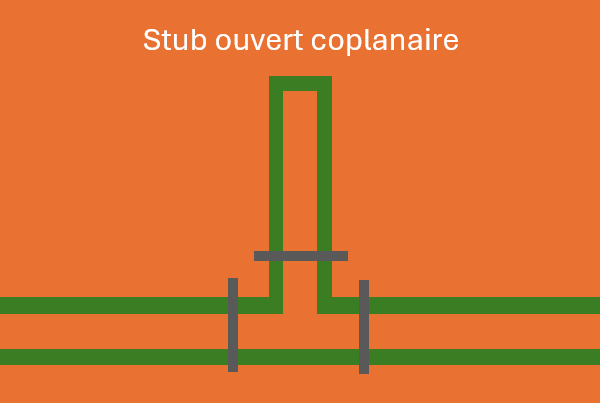
\includegraphics[width=\textwidth]{images/cpwstub.png}
        \caption{\small{Stub ouvert coplanaire}}
        \label{fig:cpwstub}
    \end{minipage}
\end{figure}

\vspace{0.5cm}
Les \textbf{figures \ref{fig:microstub}} et \textbf{\ref{fig:cpwstub}} montrent des stub microruban et coplanaire ouverts en vue du dessus. Le substrat est représenté en vert et les parties en cuivre sont représentées en orange. Dans les 2 images, la ligne de transmission traverse l'image horizontalement et le stub se trouve au centre perpendiculairement à la ligne. 

\vspace{0.5cm}
Pour le stub coplanaire, il y a en plus des ponts représentés en gris au niveau du départ du stub. Ces ponts permettent de garantir d’équipotentialité du plan de masse de part et d'autre du stub et de la ligne, et ainsi conserver un mode de propagation quasi-TEM.

\vspace{0.5cm}
Les particularités des stub sont observées à $\lambda/4$, à cette condition, les stub ouverts sont vus comme des courts-circuits et les stub en court-circuit sont vu comme ouverts. C'est ce principe qui est largement utilisé dans la réalisation de filtre, de circuit d'adaptation ou encore de résonateur en RF. 

\newpage
Ce phénomène s'explique plutôt facilement, pour le stub ouvert, l'onde arrivant au bout de ce dernier est réfléchie avec un déphasage nul (circuit ouvert). En revenant au départ du stub elle aura parcouru au total $\lambda/2$ et sera donc déphasé de 180° par rapport à l'onde sur la ligne. Les ondes vont donc s'annuler, la tension sera nulle au départ du stub et il est donc vu comme un court-circuit.

\vspace{0.5cm}
Pour le cas du stub en court-circuit, en arrivant au bout du stub, l'onde est réfléchie avec un déphasage de 180°, elle aura aussi parcouru une distance de $\lambda/2$ au total et reviendra au départ du stub avec un déphasage de 360° (soit 0°) par rapport à l'onde sur la ligne. Les ondes vont s’additionner et la tension sera maximale, le stub est donc vu comme un circuit ouvert.

\vspace{0.5cm}
Les \textbf{figure \ref{fig:openstubschema}} et \textbf{\ref{fig:shortstubschema}} en annexe montrent les schémas Qucs pour les stub ouvert et en court-circuit. Les \textbf{figures \ref{fig:openstubmeas}} et \textbf{\ref{fig:shortstubmeas}} quant à elles donnent les résultats de simulation de ces derniers. Avec du FR4 comme substrat de hauteur 1.6 mm et une largeur de piste de 3 mm. d’après les calculs effectuer précédemment, l’impédance de la ligne est de $50,79\Omega$ et la célérité de l'onde est de $1.644 \cdot 10^8$. Afin d'avoir une fréquence de coupure à 1 GHz, la longueur du stub doit être de $l = \frac{v}{4f}=41.1$ mm. 

\vspace{0.5cm}
Les résultats donnés par Qucs correspondent bien aux calculs effectuées, et on voit bien comment le stub agit soit comme un coupe bande, soit comme un passe bande. À noter que les courbes s'arrêtent dans ce cas à 2 GHz mais plus loin se trouvent les harmoniques à 3 GHz, 5 GHz, 7 GHz etc...

\vspace{1cm}
\begin{figure}[h]
    \centering
    \begin{minipage}[b]{0.445\textwidth}
        \centering
        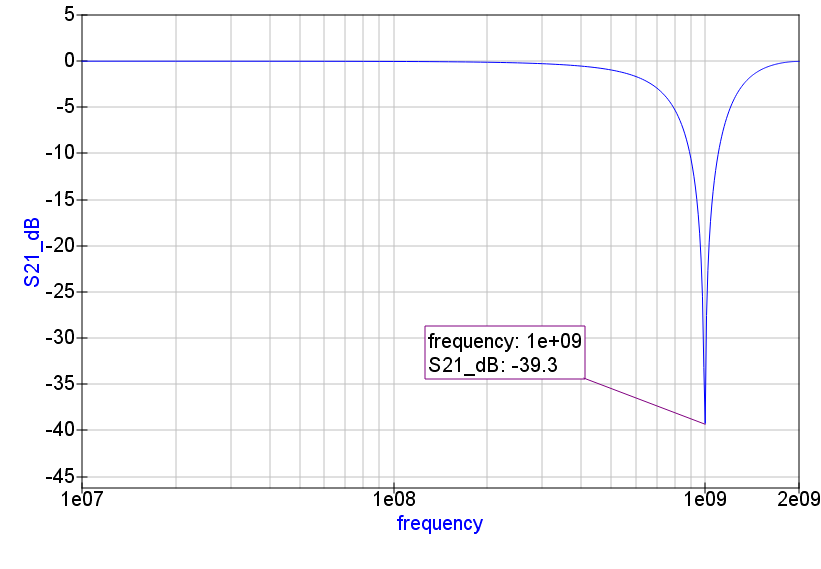
\includegraphics[width=\textwidth]{images/openstubmeas.png}
        \caption{\small{Réponse stub ouvert}}
        \label{fig:openstubmeas}
    \end{minipage}
    \hspace{0.05\textwidth}
    \begin{minipage}[b]{0.45\textwidth}
        \centering
        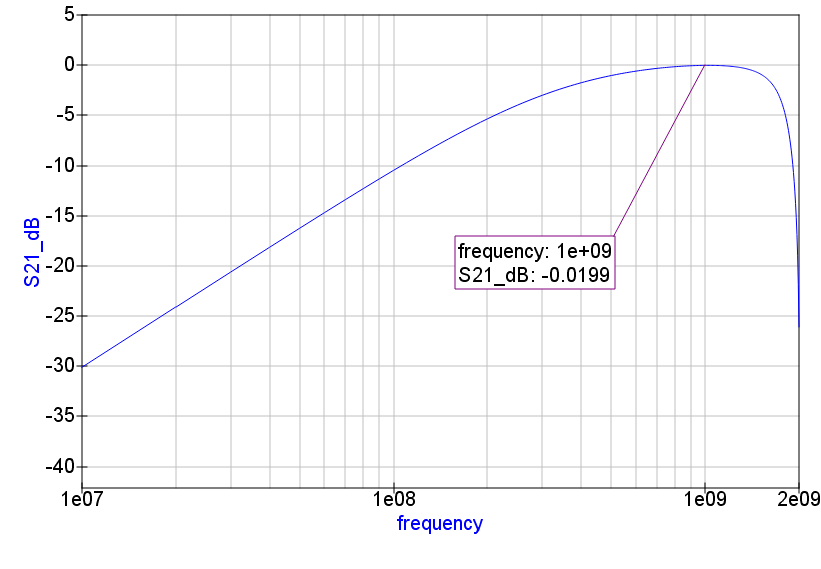
\includegraphics[width=\textwidth]{images/shortstubmeas.png}
        \caption{\small{Réponse stub en cc}}
        \label{fig:shortstubmeas}
    \end{minipage}
\end{figure}

\vspace{0.5cm}
Ces résultats de simulation se trouvent en grand format en annexe aux \textbf{figures \ref{fig:openstubmeas2}} et \textbf{\ref{fig:shortstubmeas2}}.

\newpage
Pour finir, il est important de noter que les stub peuvent parfois exister de manière parasites, les cas les plus parlant sont ceux des bus de transmission ou encore du routage des signaux d'horloge. L'article \textbf{[\ref{ref:StubClock}]} est particulièrement intéressant, on y trouve notamment des mesures comparant les 2 signaux issues des deux méthodes de routages en \textbf{figure \ref{fig:stuberror}}. 

\vspace{1cm}
\begin{figure}[h]
    \centering
    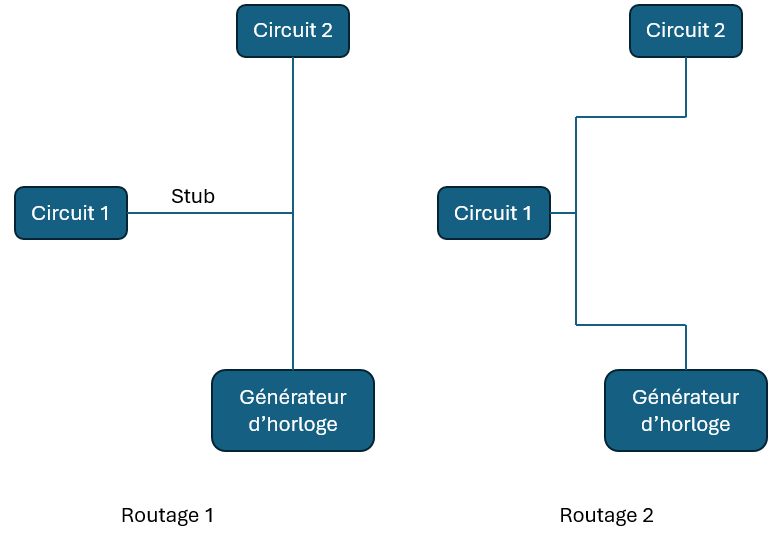
\includegraphics[scale=0.6]{images/stuberror.png}
    \caption{Stub parasite sur ligne d'horloge}
    \label{fig:stuberror}
\end{figure}

\vspace{0.5cm}
Si le signal d'horloge est à 1 Ghz, pour les 2 routages, l'adaptation d’impudence a été réalisée avec soin pour avoir 50 ohm sur un microruban de 3 mm de large. Dans le cas du routage 1 si le circuit 1 se trouve a 41 mm de la ligne principale c'est la catastrophe. En effet, les entrées logiques ont souvent une impédance élevée, si l’adaptation n'est pas faite correctement vers le circuit 1, le stub formé va alors couper complètement la fondamentale du signal carré ainsi que toutes ces harmoniques et le circuit 2 ne verra jamais l'horloge.  

\vspace{0.5cm}
Dans le cas du routage 2, la ligne principale est très proche, le stub formé est alors très court et posera des problèmes à des fréquences bien plus élevées. Ce genre d'erreur de routage peut provoquer de gros problèmes et peut être difficile à dépanner après coup. Le pire cas possible a été illustré mais une atténuation partielle du signal suffit souvent à compromettre le bon fonctionnement d'un projet entier. 

\newpage
\subsubsection{Résonateur demi onde}
Le résonateur demi onde sur ligne coplanaire agit comme un filtre passe bande. Il s'agit d'une ligne microruban ou coplanaire avec 2 fentes. Le morceaux de ligne entre les fentes entre en résonance lorsque la longueur de ce dernier vaut $\lambda/2$. Les fentes ne laissent passer qu'une faible fraction de l'énergie de l'onde mais, lorsque la ligne entre en résonance, il y a formation d’interférences constructives et la puissance devient plus élevée de manière localisée dans la ligne centrale.
La \textbf{figure \ref{fig:halfwaveex}} montre un résonateur demi onde sur une ligne coplanaire.

\vspace{0.5cm}
\begin{figure}[h]
    \centering
    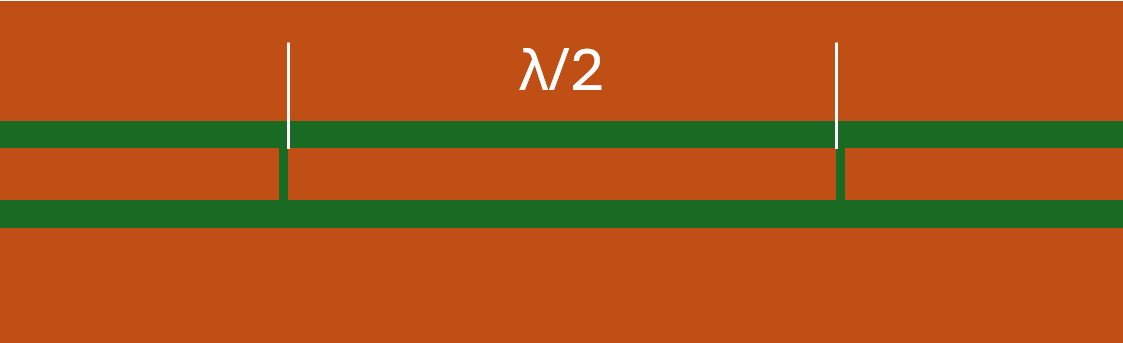
\includegraphics[scale=0.3]{images/halfwaveex.png}
    \caption{Résonateur demi onde sur ligne coplanaire}
    \label{fig:halfwaveex}
\end{figure}

\vspace{0.5cm}
Ce résonateur a été simulé sur Qucs pour une résonance à 1 GHz. D’après les calculs précédents, pour un gap de $2$ mm entre la ligne et la masse, une largeur de piste de $1.7$ mm, et les gap entourant le résonateur de $0.1$ mm, la célérité est de $1.877 \cdot 10^8$. Donc $l = \frac{C}{2f}=94.35$ mm. La ligne n'est pas parfaitement adaptée mais il est important que les gaps de part et d'autre du résonateur soient grandement inférieurs au gap entre la ligne et la masse. Malgré cette désadaptation, sur ligne seule, à 1 GHz, le paramètre S21 est à -0.2 dB ce qui reste largement acceptable. Si la fréquence du résonateur doit être plus élevée il faudra faire certaines concessions.

\vspace{0.5cm}
Le schéma Qucs se trouve à la figure \textbf{figures \ref{fig:halfqucsschema}} en annexe. La \textbf{figure \ref{fig:halfqucsmeas}} (\textbf{figure \ref{fig:halfqucsmeas2}} en grand format) donne la réponse du filtre. Le caractère d'un filtre passe bande est très visible et le facteur de qualité est bien meilleur qu'avec un stub en cour-circuit, ce résonateur nécessite cependant plus d'espace puisque que c'est un demi onde et non un quart d'onde.

\vspace{0.5cm}
\begin{figure}[h]
    \centering
    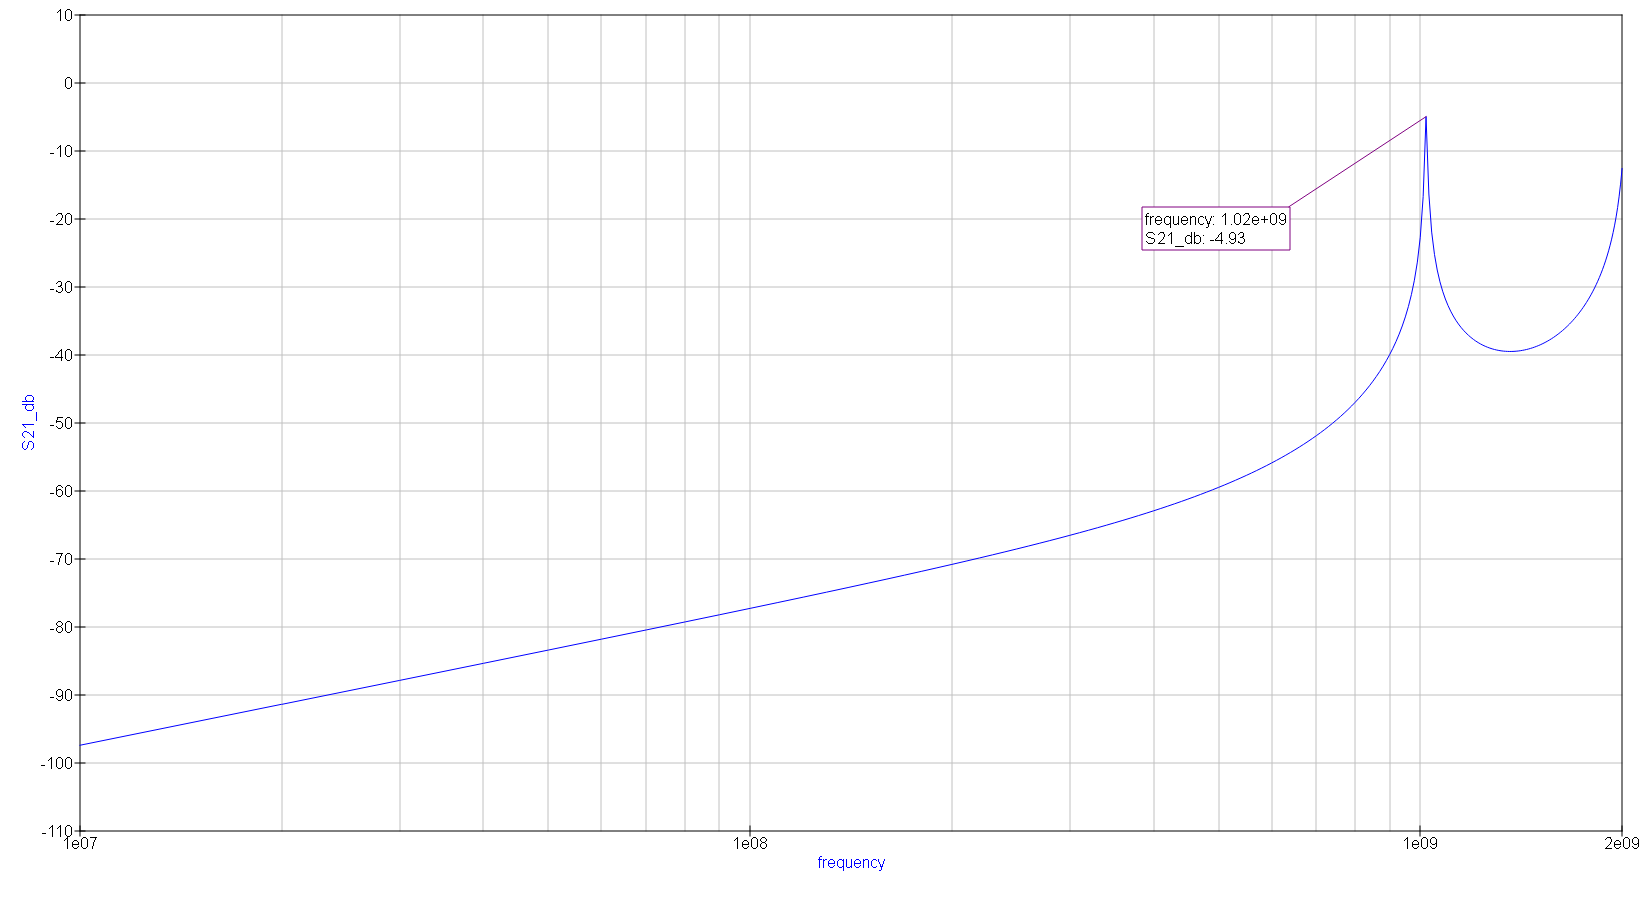
\includegraphics[scale=0.2]{images/halfqucsmeas.png}
    \caption{Réponse résonateur demi-onde}
    \label{fig:halfqucsmeas}
\end{figure}

\newpage
\section{Conception des capteurs}
\subsection{Logiciels de simulations}
Les deux logiciels de simulation utilisés dans ce travail sont Ansys HFSS (High-Frequency Structure Simulator) et Qucs (Quite Universal Circuit Simulator). Ces logiciels permettent tout deux de simuler des circuits RF mais avec des approches très différentes. Au sein du projet, ce sont surtout les paramètres S qui sont intéressant, et plus particulièrement le S21 qui est la transmission, mais ces logiciels de calculs sont capable de bien plus.

\vspace{1cm}
\subsubsection{Qucs}
Qucs de son coté se rapproche plus d'un logiciel de simulation de circuit dit classique. La \textbf{figure \ref{fig:openstubschema2}} par exemple montre à quoi ressemble un schéma sur qucs. Afin de réaliser son schéma sur qucs on y place simplement différents types de composants afin de former un circuit, ou plus précisément dans le cas de ce projet, une structure RF. En effet, contrairement à la majorité des logiciels de simulation de circuit, Qucs possède, en plus des composants classiques, des structures RF pré-calculées. Il possède notamment des lignes microruban et coplanaire, en arrangeant ces simples structures il est possible de créer des structures bien plus complexes. 

\vspace{1cm}
\begin{figure}[h]
    \centering
    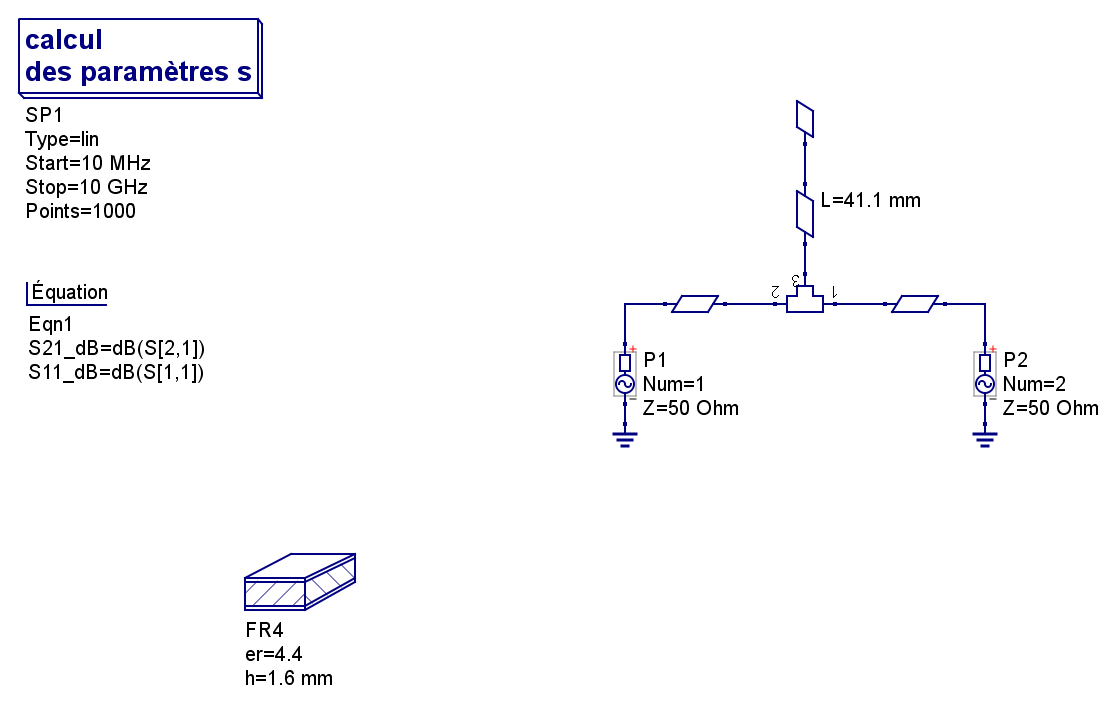
\includegraphics[scale=0.5]{images/openstubschema.png}
    \caption{Schéma Qucs stub ouvert}
    \label{fig:openstubschema2}
\end{figure}

\newpage
Les informations détaillées du fonctionnement de Qucs se trouvent dans le document \textbf{[\ref{ref:QucsTech}]}. Comme expliqué précédemment, Qucs possède des blocs qui sont pré-calculés, autrement dit, Qucs connaît les paramètres S de ces blocs en fonction des paramètres qui lui sont attribué. Afin de calculer les paramètres du circuit entier, il parcourt le schéma bloc par bloc et calcule les paramètres totaux en mettant les blocs ensemble un à un.

\vspace{0.5cm}
Pour mettre ces blocs ensemble, différents paramètres sont utilisés dépendamment des configurations présentées en \textbf{figure \ref{fig:QucsPortMatching}}:

\begin{itemize}[leftmargin=2cm, label=\textbullet]
    \item Paramètre Y : connexion parallèle-parallèle
    \item Paramètre Z : connexion série-série
    \item Paramètre H : connexion série-parallèle
    \item Paramètre G : connexion parallèle-série
    \item Paramètre ABCD : connexion cascade
\end{itemize}

\vspace{1cm}
\begin{figure}[ht]
    \centering
    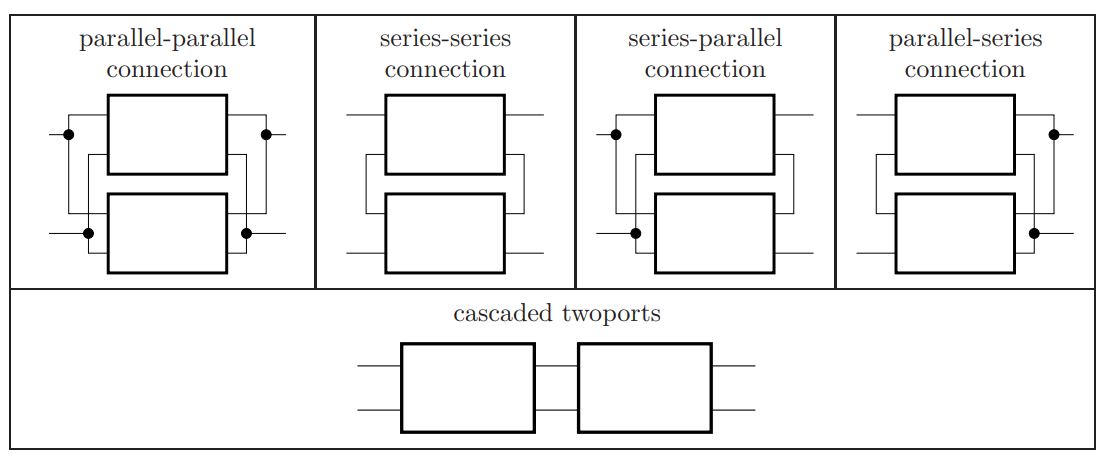
\includegraphics[width=0.6\linewidth]{images/QucsPortMatching.png}
    \caption{Interconnexion des réseaux}
    \label{fig:QucsPortMatching}
\end{figure}

\vspace{0.5cm}
Cette méthode de calcul présente l'avantage d'être extrêmement rapide. En effet, une simulation sur Qucs se fait facilement en moins d'une seconde pour les structures de ce projet. Malgré cette rapidité, les résultats restent très précis et proches de la réalité, en fonction du composant et des formules utilisées le document \textbf{[\ref{ref:QucsTech}]} garanti dans la majorité des cas une précision inférieure à $\pm$1\%.

\vspace{0.5cm}
Le point faible de Qucs et de sa méthode de calcul est qu'elle restreint grandement l'utilisateur. En effet, puisqu'il utilise des blocs pré-calculés, les paramètres ne sont pas illimité et des structures qui sortent de l'ordinaire ne sont souvent pas réalisable. Dans ce travail Qucs a permis de bonne et rapide approximation mais Ansys HFSS est plus précis puisque la majorité des structures sortent du classique. 

\newpage
\subsubsection{Ansys HFSS}
Ansys HFSS est le second logiciel de simulation utilisé pour le projet, et fonctionne de façon très différente à Qucs. Au premier abord, HFSS ressemble plus à un logiciel de CAO, il permet de créer une multitude de formes en trois dimensions. La \textbf{figure \ref{fig:HFSS_Example}} est un exemple de ligne coplanaire réalisée avec Ansys HFSS.

\vspace{1cm}
\begin{figure}[h]
    \centering
    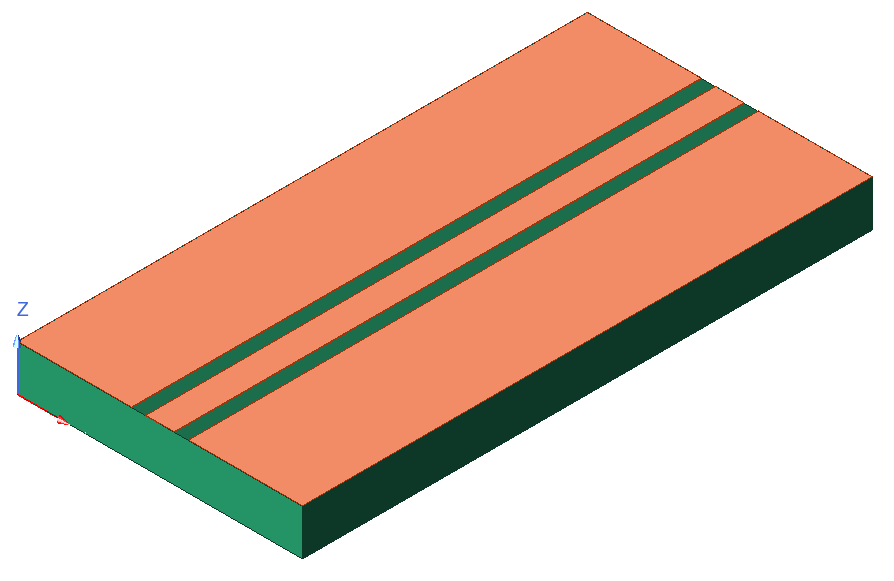
\includegraphics[scale=0.4]{images/HFSS_Example.png}
    \caption{Exemple de ligne coplanaire sur Ansys HFSS}
    \label{fig:HFSS_Example}
\end{figure}

\vspace{0.5cm}
La méthode de calcul qu'utilise HFSS est donnée dans le document \textbf{[\ref{ref:HFSStech}]}. HFSS utilise la méthode des éléments finis. Pour commencer, il définit les paramètres de simulation complets incluant les paramètre des matériaux, les conditions aux limites, les ports etc...  Ensuite il décompose la structure en une multitude de tétraèdres qui constituent un maillage. Les équations de chacune des mailles sont ensuite assemblées pour résoudre le système tout en satisfaisant les équations différentielles vectorielles de Maxwell sur l'ensemble du domaine. 

\vspace{0.5cm}
Si l'erreur sur les paramètres S estimés est trop élevée, HFSS adapte le maillage automatiquement, le logiciel va répéter ces étapes en boucle jusqu’à atteindre les critères de convergences ou le nombre maximal d’itération fixé par l'utilisateur.

\vspace{0.5cm}
Cette méthode à l'avantage de permettre de caractérisé n'importe quel structure, aussi complexe qu'elle puisse être, pour autant que le maillage soit bien réalisé. Cependant elle est coûteuse en puissance de calculs et les temps de simulation peuvent s’avérer très long.

\newpage
\subsection{Capteurs}
Lors de la réalisation des capteurs, la suite démontre qu'il est possible de détecter la présence d'eau à l'aide de l’électronique RF. Cependant, l'implémentation reste très compliquée. Afin que le jet n'entre pas en contact avec le PCB, le trou par lequel le jet passe doit être de diamètre grandement supérieure au diamètre du jet. Le couplage électromagnétique est alors grandement réduit, et le jet n'induit pas une variation assez élevée pour qu'il soit mesurable.

\vspace{0.5cm}
Selon moi, une collaboration avec des ingénieurs spécialistes en matériaux et mécanique des fluides devient indispensable afin de trouver l'implémentation parfaite de la structure RF sur la sortie du jet d'eau.

\newpage
\subsubsection{Stub microruban 1 GHz}
Le premier capteur mis en œuvre est un simple stub microruban avec une fréquence de coupure à 1 GHz. L'objectif étant de détecter la présence d'eau statique à l’extrémité de ce dernier. Dans un premier temps il a été simulé sur Qucs et Ansys HFSS. Qucs ne permettant pas de changer le substrat au bout du stub comme souhaité, il a simplement permis de vérifier la longueur et la correspondance avec la fréquence de résonance. 

\vspace{0.5cm}
Ce circuit a été réalisé au sein de l'HEPIA sur un graveuse de PCB. Le substrat est du FR4 de 1.6 mm d'épaisseur, le cuivre à une épaisseur soit de 18 micron soit de 35 micron mais cela n'a que peu d'importance pour le stub microruban. Avec ces paramètres, la ligne doit avoir une largeur de 3 mm afin d'avoir un impédance de 50 ohm et le stub doit faire 41.1 mm. 

\vspace{0.5cm}
La \textbf{figure \ref{fig:Qucs_Stub_1}} montre le schéma du stub dans Qucs. On y retrouve la longueur du stub et la \textbf{figure \ref{fig:Qucs_Stub_1_Mmeas}} confirme avec les résultats que la longueur du stub est correct.

\vspace{1cm}
\begin{figure}[h]
    \centering
    \begin{minipage}[b]{0.445\textwidth}
        \centering
        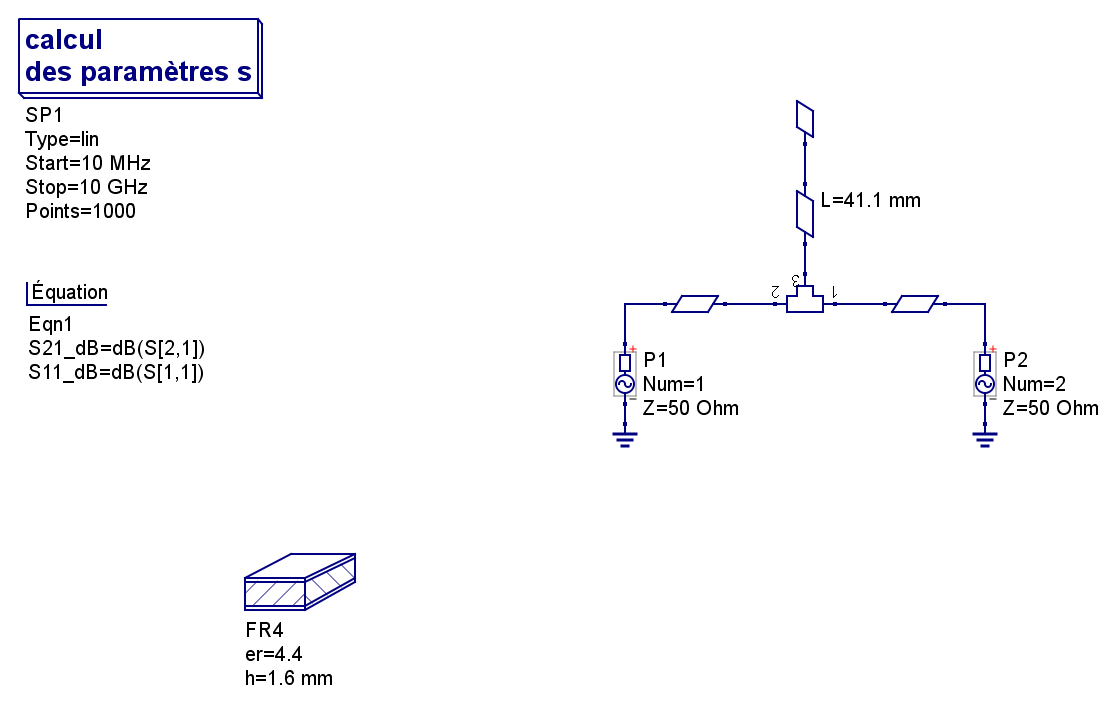
\includegraphics[width=\textwidth]{images/openstubschema.png}
        \caption{\small{Schéma Qucs stub microruban 1 GHz}}
        \label{fig:Qucs_Stub_1}
    \end{minipage}
    \hspace{0.05\textwidth}
    \begin{minipage}[b]{0.45\textwidth}
        \centering
        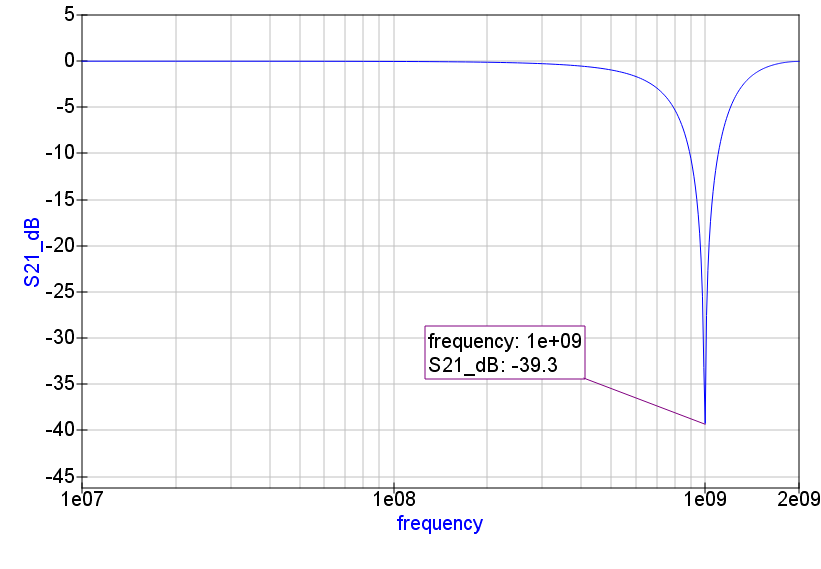
\includegraphics[width=\textwidth]{images/openstubmeas.png}
        \caption{\small{Résultats Qucs stub microruban 1 GHz}}
        \label{fig:Qucs_Stub_1_Mmeas}
    \end{minipage}
\end{figure}

\vspace{1cm}
Par la suite, une simulation plus précise a été réalisée avec Ansys HFSS. La \textbf{figure \ref{fig:HFSS_Stub_1}} montre le design réalisé sur HFSS. Il a permis en plus de la simulation sur qucs, d'y ajouter un trou puis de simuler le comportement avec et sans eau.

\newpage
\vspace{1cm}
\begin{figure}[h]
    \centering
    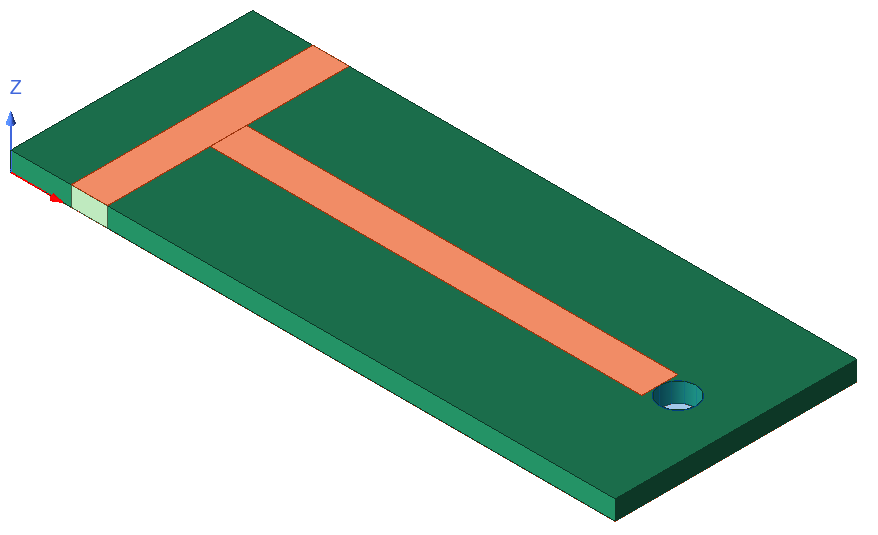
\includegraphics[scale=0.4]{images/HFSS_Stub_1.PNG}
    \caption{Stub microruban 1 GHz sur Ansys HFSS}
    \label{fig:HFSS_Stub_1}
\end{figure}

\vspace{1cm}
Les simulations sur HFSS donnent les résultats présents aux \textbf{figures \ref{fig:stub_1_HFSS_Result}} et \textbf{\ref{fig:stub_1_HFSS_Result_wat}}. On peut constater une légère variation de la fréquence de coupure du stub. Cela s'explique par le fait qu'en remplaçant l'air au bout du stub par de l'eau, sa longueur effective varie légèrement, impliquant une variation sur la fréquence de coupure.

\vspace{1cm}
\begin{figure}[h]
    \centering
    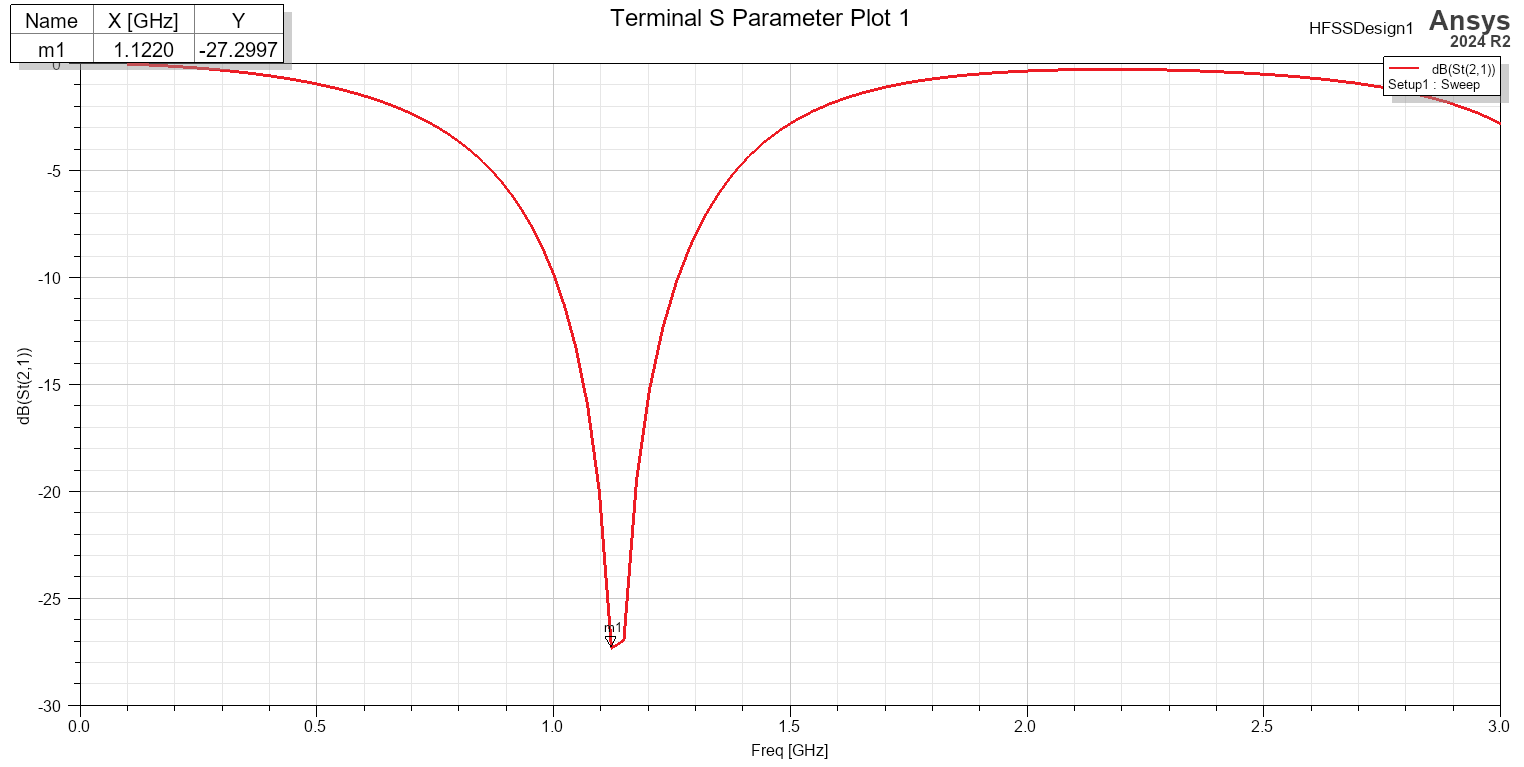
\includegraphics[scale=0.2]{images/S21_SansEau.png}
    \caption{Réponse simulée sans eau}
    \label{fig:stub_1_HFSS_Result}
\end{figure}

\newpage
\begin{figure}[h]
    \centering
    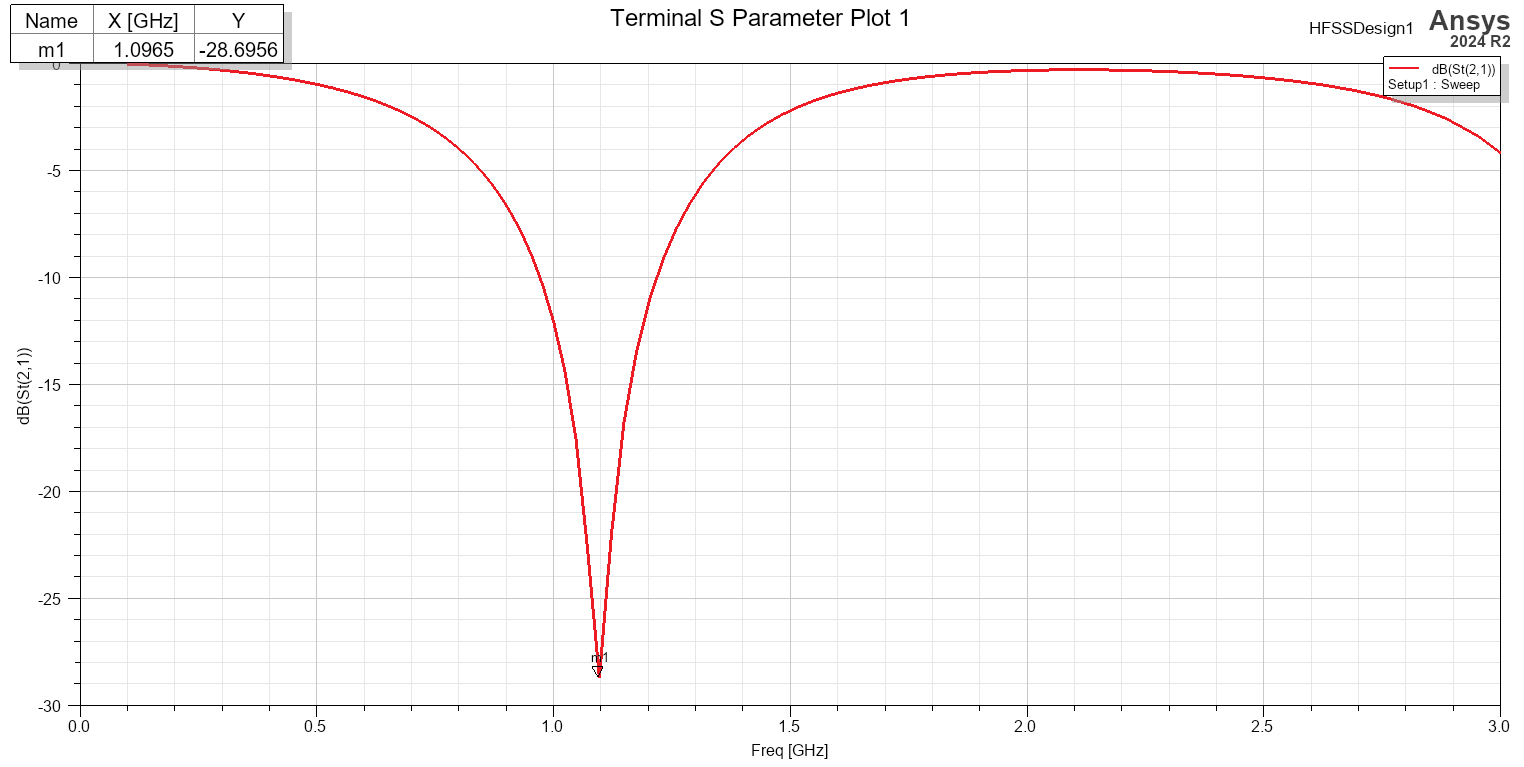
\includegraphics[scale=0.2]{images/S21_AvecEau.png}
    \caption{Réponse simulée avec eau}
    \label{fig:stub_1_HFSS_Result_wat}
\end{figure}

\vspace{1cm}
Les simulations effectuées avec HFSS montrent une variation de la fréquence de coupure allant de 1.1220 GHz à 1.0965 GHz induisant une variation de 25.5 MHz.

\vspace{0.5cm}
La \textbf{figure \ref{fig:Stub_1}} montre le circuit imprimé réalisé. Afin de mesurer réellement les effets de l'eau sur le stub en RF, une résine a été coulée pour éviter tout court circuit entre stub et la masse. Un morceau de scotch a été collé du coté de la masse afin de réaliser un petit récipient pour l'eau.

\vspace{1cm}
\begin{figure}[h]
    \centering
    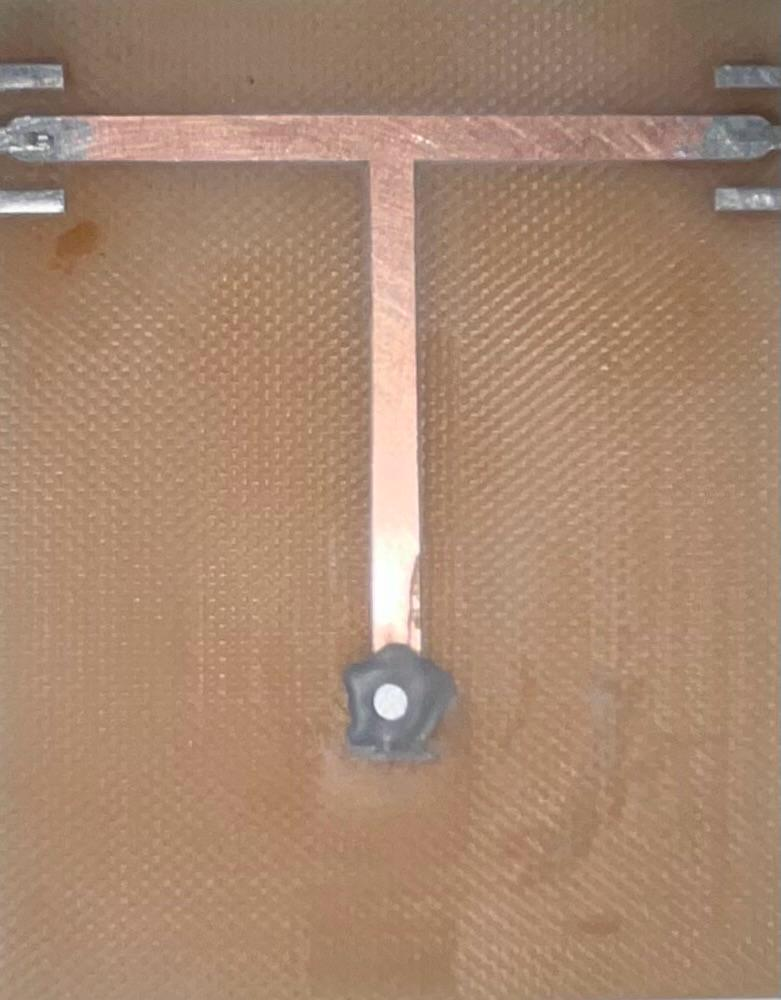
\includegraphics[scale=0.3, angle=90]{images/Stub_1.jpeg}
    \caption{Stub microruban 1 GHz}
    \label{fig:Stub_1}
\end{figure}

\newpage
À l'aide du VNA, la réponse en fréquence du stub réalisé a pu être déterminée. La \textbf{figure \ref{fig:microruban_1_compare}} compare les deux courbes au point critique. La variation est visible mais reste très légère, la fréquence de coupure passant de 1.151 GHz à 1.142 GHz, à ces fréquences cela ne représente une variation que de 0.78\%.

\vspace{0.5cm}
\begin{figure}[h]
    \centering
    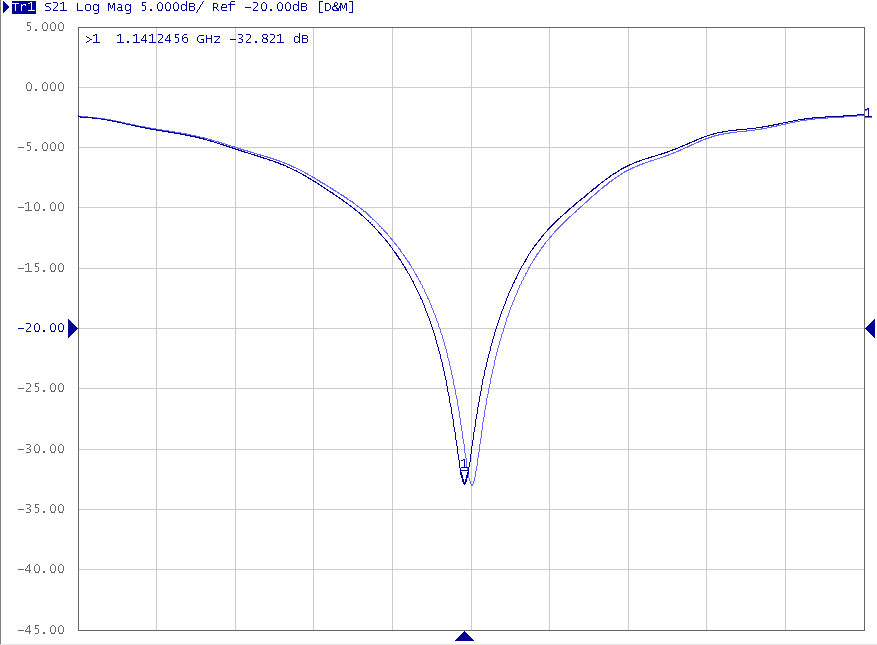
\includegraphics[scale=0.3]{images/microruban_1_compare.PNG}
    \caption{Comparaison des réponses du stub microruban avec et sans eau}
    \label{fig:microruban_1_compare}
\end{figure}

\newpage
\subsubsection{Stub coplanaire 1 GHz}
Le second capteur réalisé est un Stub coplanaire à 1 GHz. L'amélioration par rapport à son prédécesseur réside dans l'interaction entre le champ et la matière. Les \textbf{figures \ref{fig:inter_champ_micro}} et \textbf{\ref{fig:inter_champ_cpw}} montrent cette différence d'interaction. Ce sont des vues en coupe du bout du stub avec l'eau représentée en bleu, le champ électrique représenté en rouge. Ont constate rapidement avec ces schémas que le microruban n'est pas la solution optimale pour concentrer le champ dans le fluide. D'autant plus que le fluide sera voué à traverser le PCB et ne sera pas une goutte posée dessus. En noir, on retrouve le scotch sous le PCB expliquer dans la section précédente et en violet la couche de résine. 

\vspace{0.5cm}
\begin{figure}[h]
    \centering
    
\includegraphics[scale=0.3]{images/inter_champ_micro.png}
    \caption{Interaction stub microruban}
    \label{fig:inter_champ_micro}
\end{figure}

\vspace{0.5cm}
\begin{figure}[h]
    \centering
    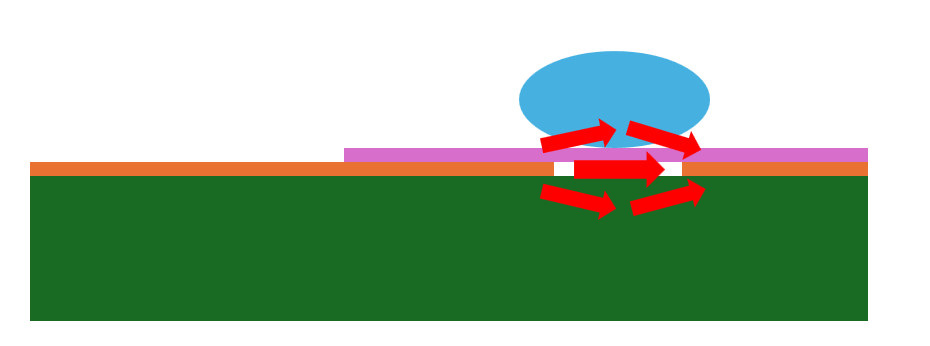
\includegraphics[scale=0.4]{images/inter_champ_cpw.png}
    \caption{Interaction stub coplanaire}
    \label{fig:inter_champ_cpw}
\end{figure}

\vspace{0.5cm}
Comme pour le capteur précédent, le PCB a été gravé à l'HEPIA. Les paramètres sont les mêmes que pour le stub avec une épaisseur de cuivre fixé de 18 microns et la contrainte de la taille minimale de gravure qui est de 0.2 mm. Autrement dit, le gap entre la ligne et la masse doit être de 0.2 mm au minimum. 

\vspace{0.5cm}
Le stub coplanaire mis en œuvre pour ce capteur possède un gap de 0.3 mm et une largeur de piste de 2.2 mm afin de garantir l'impédance de 50 ohm. Avec ces conditions, le stub doit faire une longueur de 74.53 mm.

\newpage
Comme pour le cas précédent des premières simulations sur Qucs ont permis de valider le design rapidement. Le schéma et la réponse du stub coplanaire sur qucs se trouvent en \textbf{figures \ref{fig:Qucs_StubCPW_1_schema}} et \textbf{\ref{fig:Qucs_StubCPW_1_meas}}. La fréquence de coupure se trouve bien à 1 GHz.

\vspace{1cm}
\begin{figure}[h]
    \centering
    \begin{minipage}[b]{0.445\textwidth}
        \centering
        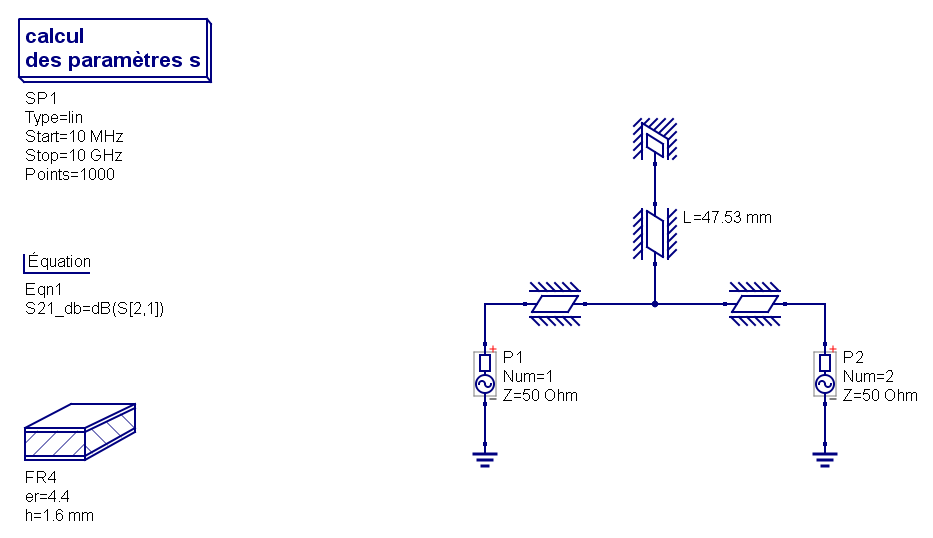
\includegraphics[width=\textwidth]{images/Qucs_StubCPW_1_schema.png}
        \caption{\small{Schéma Qucs stub coplanaire 1 GHz}}
        \label{fig:Qucs_StubCPW_1_schema}
    \end{minipage}
    \hspace{0.05\textwidth}
    \begin{minipage}[b]{0.45\textwidth}
        \centering
        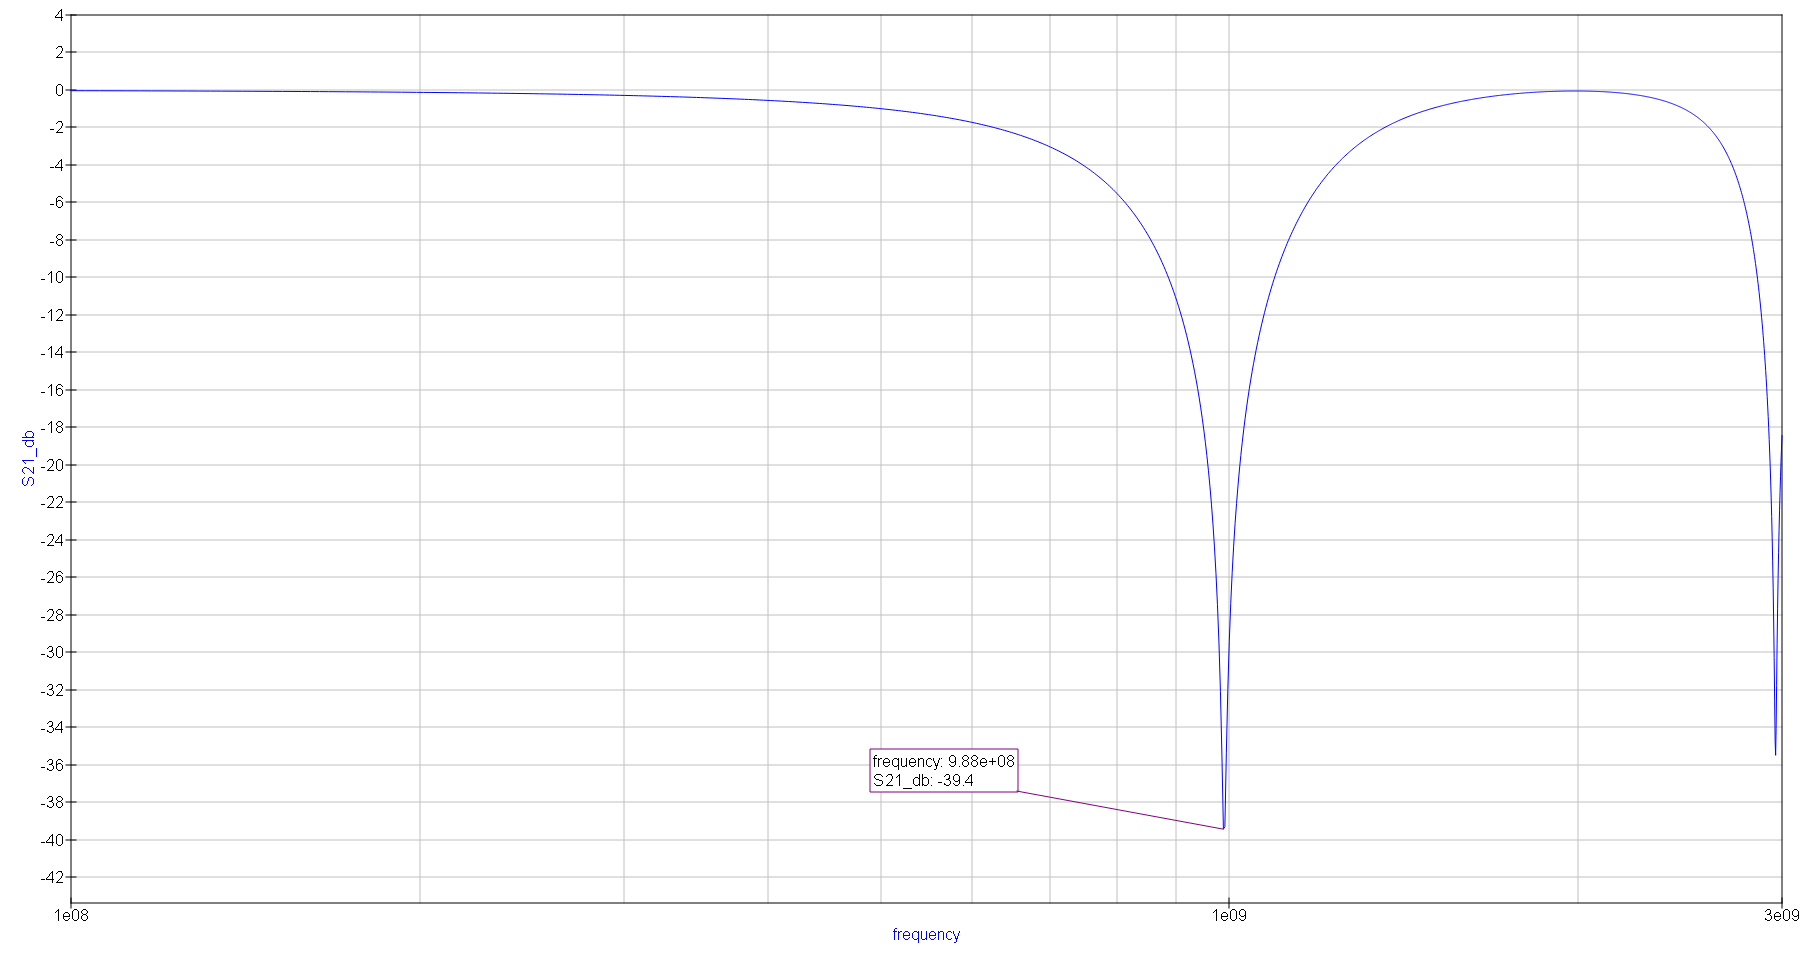
\includegraphics[width=\textwidth]{images/Qucs_StubCPW_1_meas.png}
        \caption{\small{Résultats Qucs stub coplanaire 1 GHz}}
        \label{fig:Qucs_StubCPW_1_meas}
    \end{minipage}
\end{figure}

\vspace{0.5cm}
Ensuite, ce capteur a été testé en conditions réelles sans passer par la case HFSS. La \textbf{figure \ref{fig:Stub_cpw_1}} montre le PCB réalisé. Un spray protecteur, à base de résine,transparente spécialement conçue pour circuit imprimé, a été appliqué au bout du stub sur le dessus du PCB. Cela à permis d'isoler le stub et la masse afin de déposer une goutte d'eau comme sur la \textbf{figure \ref{fig:inter_champ_cpw}}.

\vspace{1cm}
\begin{figure}[h]
    \centering
    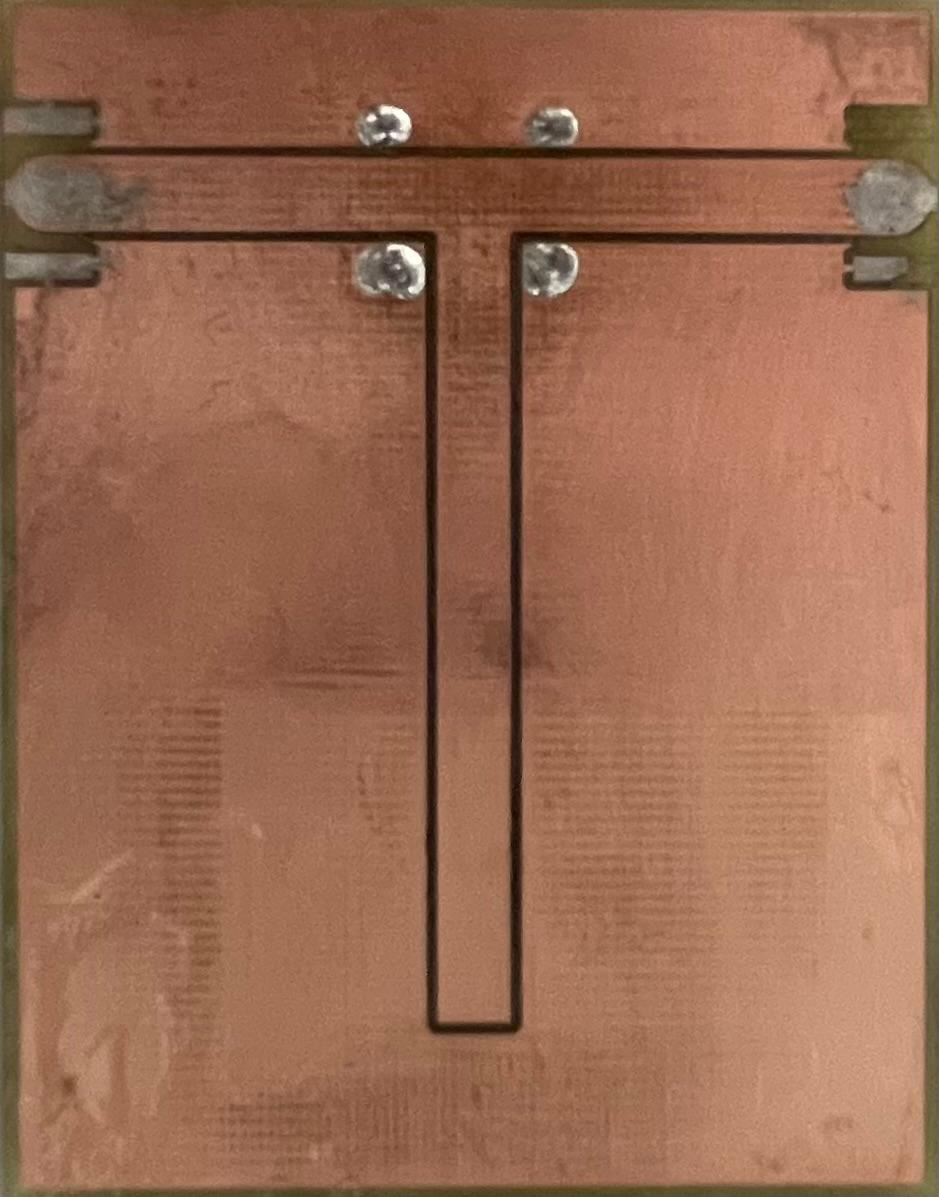
\includegraphics[scale=0.2, angle=90]{images/Stub_cpw_1.jpeg}
    \caption{Stub coplanaire 1 GHz}
    \label{fig:Stub_cpw_1}
\end{figure}

\newpage
Le VNA a permis de caractériser la réponse en fréquence de ce nouveau capteur avec et sans la goutte d'eau. La \textbf{figure \ref{fig:cpw_1_compare}} permet de comparer la réponse du circuit avec et sans la goutte. La fréquence de coupure passe de 1.023 GHz à 983.52 MHz, ce qui donne une variation relative de 3.86\%. Non seulement c'est plus élevé que pour le stub microruban mais la quantité d'eau est aussi plus faible ce second capteur semble bien plus efficace le premier. En effet, dans le capteur microruban la quantité d'eau était environ de $1.6\cdot \frac{2.6}{2}^2 \cdot \pi = 8.5mm^3$ (volume du cylindre en bout de stub). Dans le cas de ce second capteur, c'est une goûte de 1.6 de diamètre mm qui a été déposée, avec le volume d'une sphère cela donne $\frac{4}{3}\cdot\pi\cdot \frac{1.6}{2}^3 = 6.4mm^3$. On a donc un volume 24\% inférieur pour la mesure sur ce second capteur.

\vspace{1cm}
\begin{figure}[h]
    \centering
    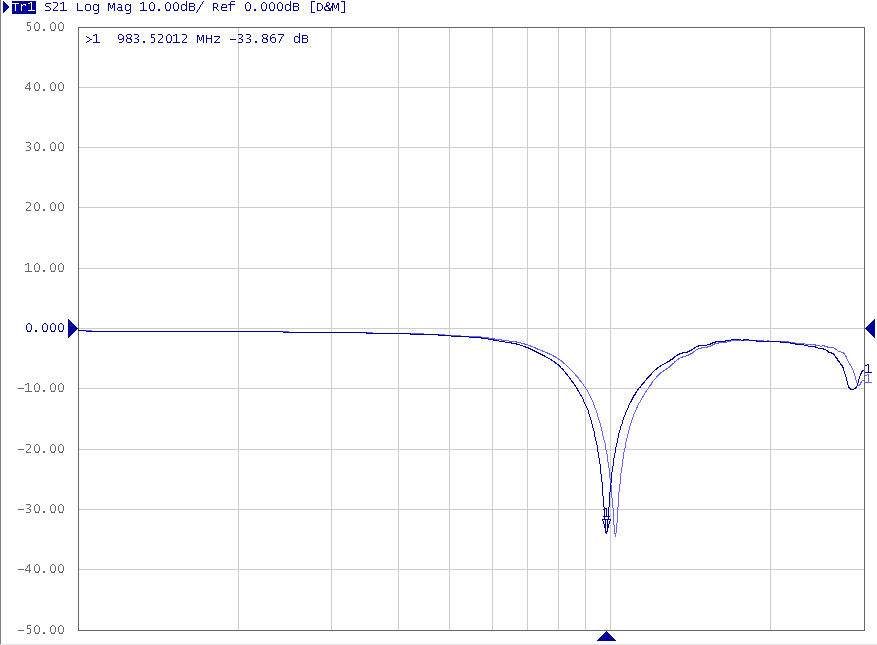
\includegraphics[scale=0.4]{images/cpw_1_compare.PNG}
    \caption{Comparaison des réponses du stub coplanaire 1 GHz avec et sans eau}
    \label{fig:cpw_1_compare}
\end{figure}

\newpage
\subsubsection{Stub coplanaire 2.5 GHz}
Ce troisième capteur est de nouveau un stub coplanaire. Cette fois ci il est conçu avec un fréquence de coupure de 2.5 GHz afin de se trouver dans la bande ISM. Le principe reste similaire au stub précédent cependant au lieu de détecter une goutte, il s'agit désormais de détecter la présence ou non du fluide, envoyé par une des vannes fournies par FAS.

\vspace{0.5cm}
Il est réalisé avec les mêmes paramètres que le stub coplanaire de 1 GHz à l’exception près de la longueur du stub. Pour avoir une fréquence de coupure à 2.5 GHz, le stub doit avoir une longueur de 19.01 mm.

\vspace{0.5cm}
Comme ces prédécesseurs, la première étape est celle de la vérification sur qucs, les \textbf{figures \ref{fig:Qucs_StubCPW_25_schema}} et \textbf{\ref{fig:Qucs_StubCPW_25_meas}}, sont le schéma et le résultat de simulation sur Qucs. Le stub a bel et bien la fréquence de coupure attendue de 2.5 GHz.

\vspace{1cm}
\begin{figure}[h]
    \centering
    \begin{minipage}[b]{0.445\textwidth}
        \centering
        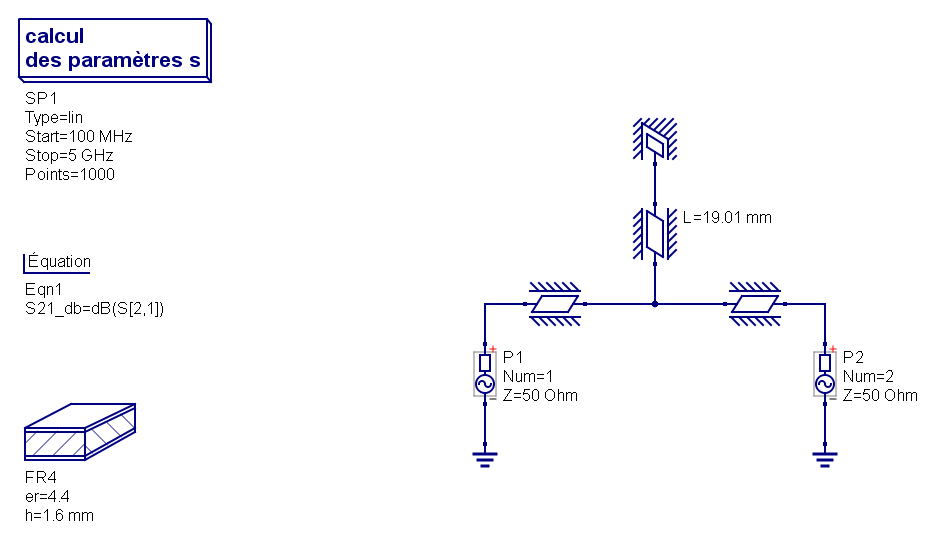
\includegraphics[width=\textwidth]{images/Qucs_StubCPW_25_schema.png}
        \caption{\small{Schéma Qucs stub coplanaire 2.5 GHz}}
        \label{fig:Qucs_StubCPW_25_schema}
    \end{minipage}
    \hspace{0.05\textwidth}
    \begin{minipage}[b]{0.45\textwidth}
        \centering
        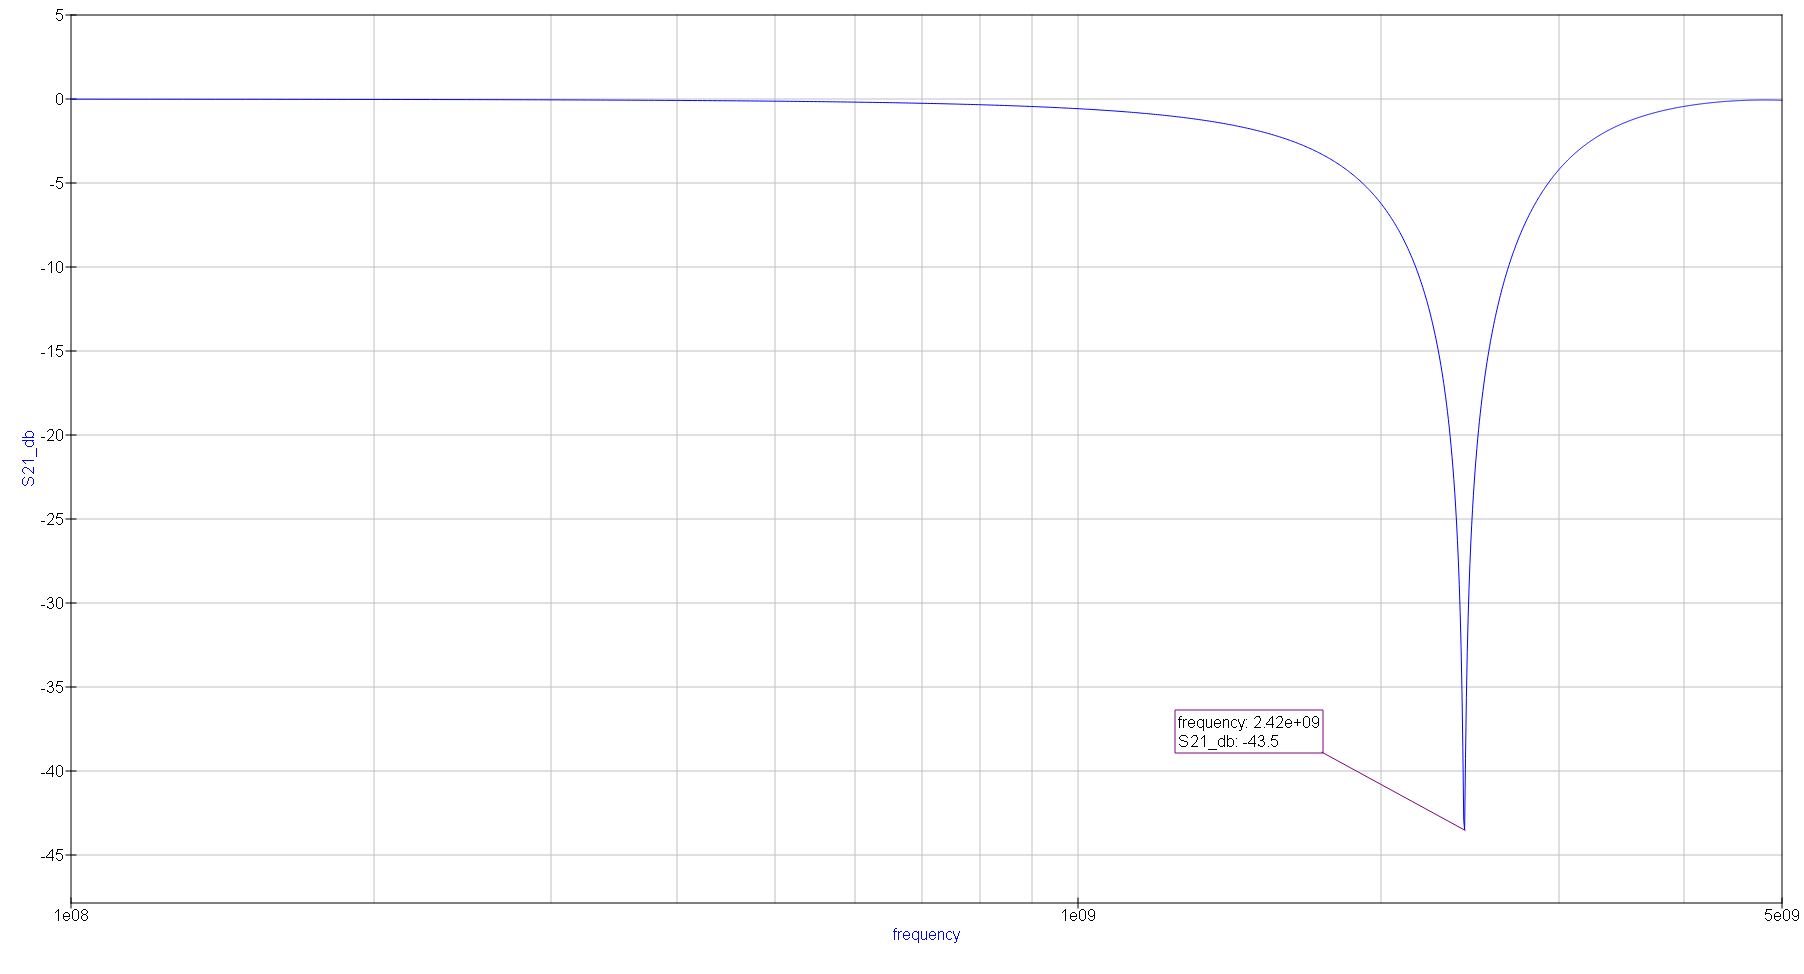
\includegraphics[width=\textwidth]{images/Qucs_StubCPW_25_meas.png}
        \caption{\small{Résultats Qucs stub coplanaire 2.5 GHz}}
        \label{fig:Qucs_StubCPW_25_meas}
    \end{minipage}
\end{figure}

\vspace{1cm}
Suite à cela il a ensuite été réalisé sur HFSS. Son design HFSS est présent à la \textbf{figure \ref{fig:stub_25_HFSS}}. Puisque l'objectif est de faire en sorte de détecter la présence du jet d'eau produit par la micro-vanne, HFSS a permis de simuler le design avec le trou. La grande colonne d'eau représente le jet d'eau constant.  

\newpage
\begin{figure}[h]
    \centering
    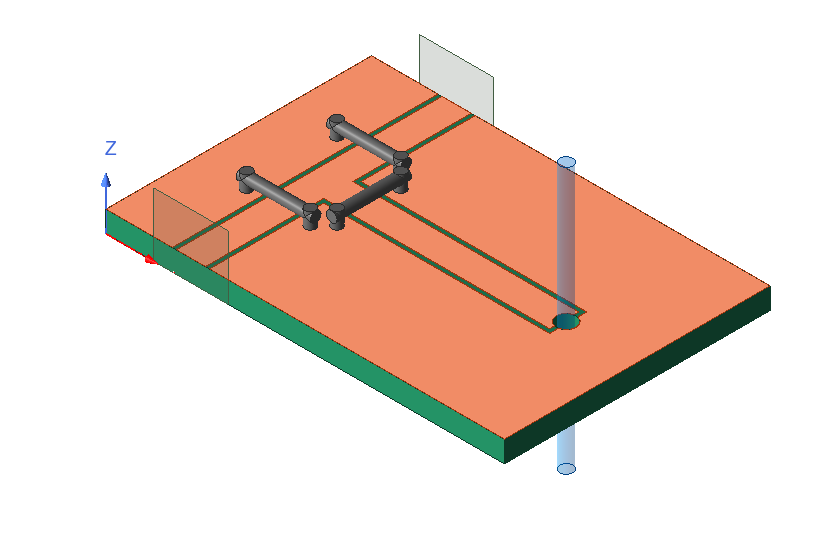
\includegraphics[scale=0.4]{images/stub_25_HFSS.png}
    \caption{Stub coplanaire 2.5 GHz sur Ansys HFSS}
    \label{fig:stub_25_HFSS}
\end{figure}

La contrainte en sortie de vanne fournie par FAS possède un diamètre de 150 microns. Pour des modèles de si petite taille, il est nécessaire de paramétrer le maillage précisément. Sachant que le logiciel a été découvert durant le projet, mes compétences sur le logiciel ne sont largement pas suffisantes pour réaliser une simulation valable. Sachant cela les simulations sont réalisées avec un jet d'eau de 1 mm de diamètre. 

\vspace{0.5cm}
Les résultats des simulations se trouvent en \textbf{figures \ref{fig:cpw_25_sansEau}} et \textbf{\ref{fig:cpw_25_avecEau}}

\vspace{1cm}
\begin{figure}[h]
    \centering
    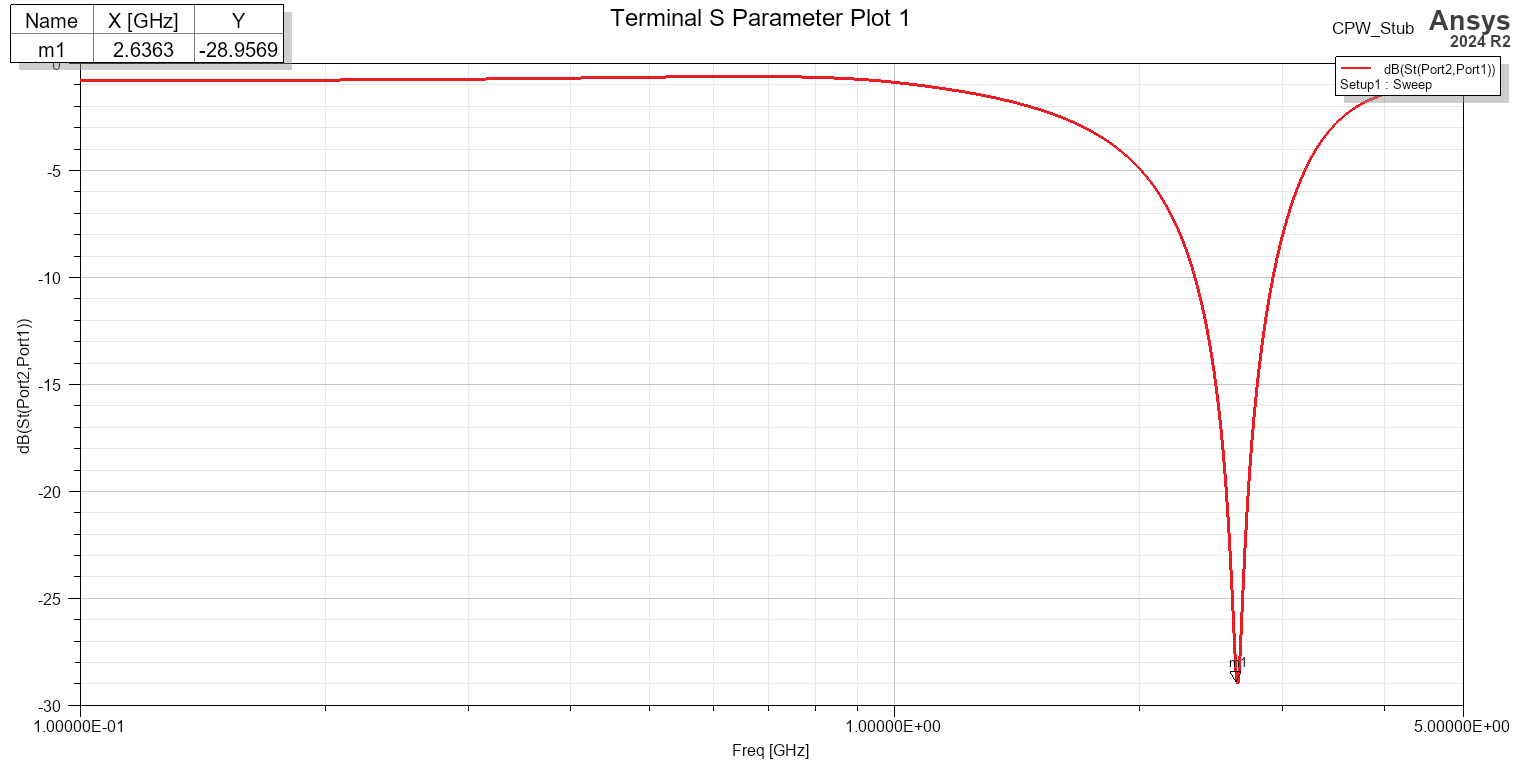
\includegraphics[scale=0.28]{images/cpw_25_sansEau.png}
    \caption{Réponse simulée sur HFSS sans jet d'eau}
    \label{fig:cpw_25_sansEau}
\end{figure}

\newpage
\begin{figure}[h]
    \centering
    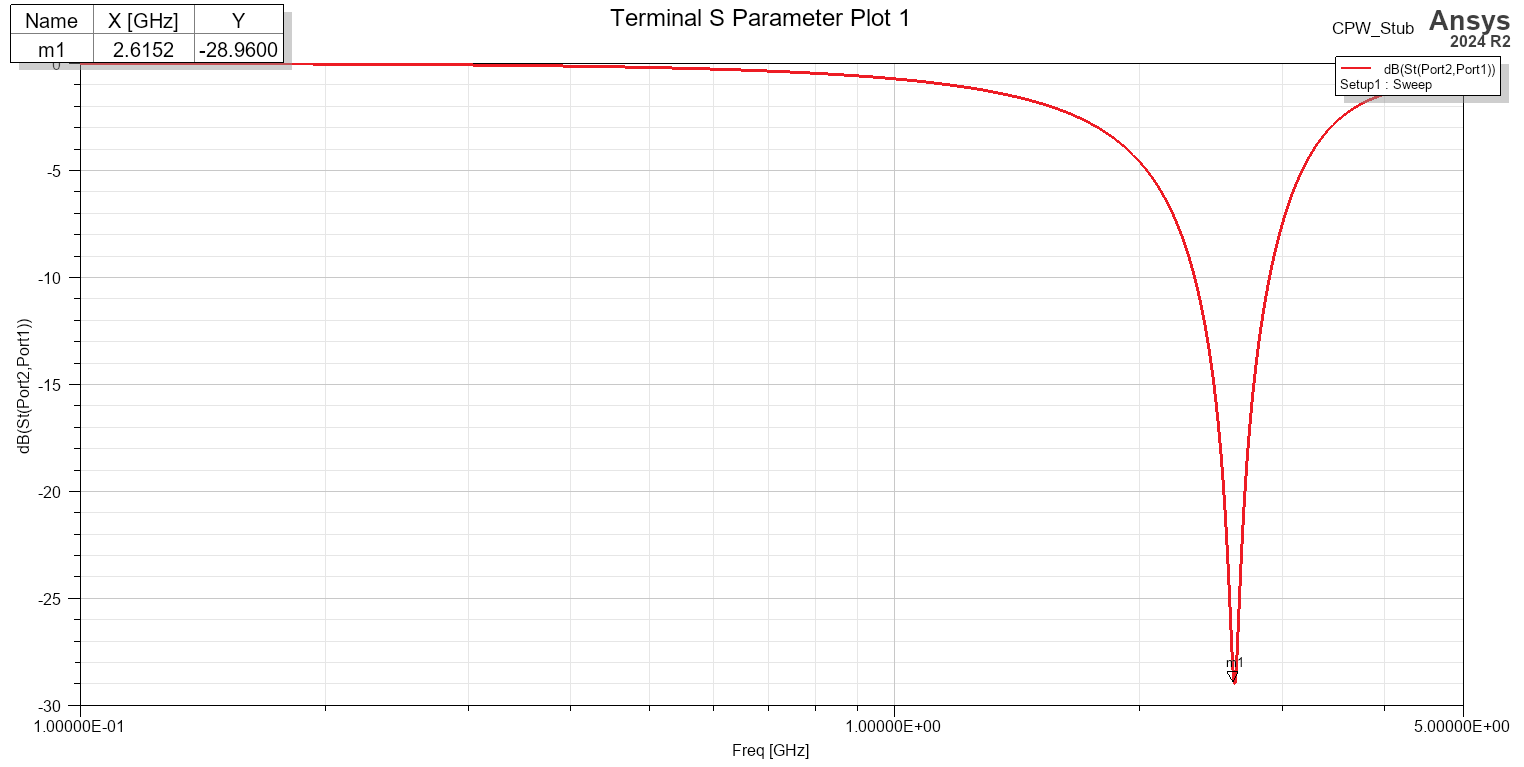
\includegraphics[scale=0.28]{images/cpw_25_avecEau.png}
    \caption{Réponse simulée sur HFSS avec jet d'eau}
    \label{fig:cpw_25_avecEau}
\end{figure}

\vspace{1cm}
Malgré le diamètre du jet élevé, la variation de la fréquence de résonance est très faible. Elle passe de 2.6363 GHz à 2.6152 GHz, ce qui représente un écart relatif de seulement 0.8\%.

\vspace{0.5cm}
Le capteur \textbf{(figure \ref{fig:cpw_25_rel})} a pu être caractérisé à l'aide du VNA, mais malheureusement la présence est indétectable et il n'est pas possible de faire la différence entre le bruit ou une variation réelle. Des mesures avec un jet de diamètre de 1 mm ont été tentées cependant l'eau s'accroche trop facilement au PCB par capillarité. La mesure du capteur est représentée en \textbf{figure \ref{fig:cpw_25_mes}}.

\begin{figure}[h]
    \centering
    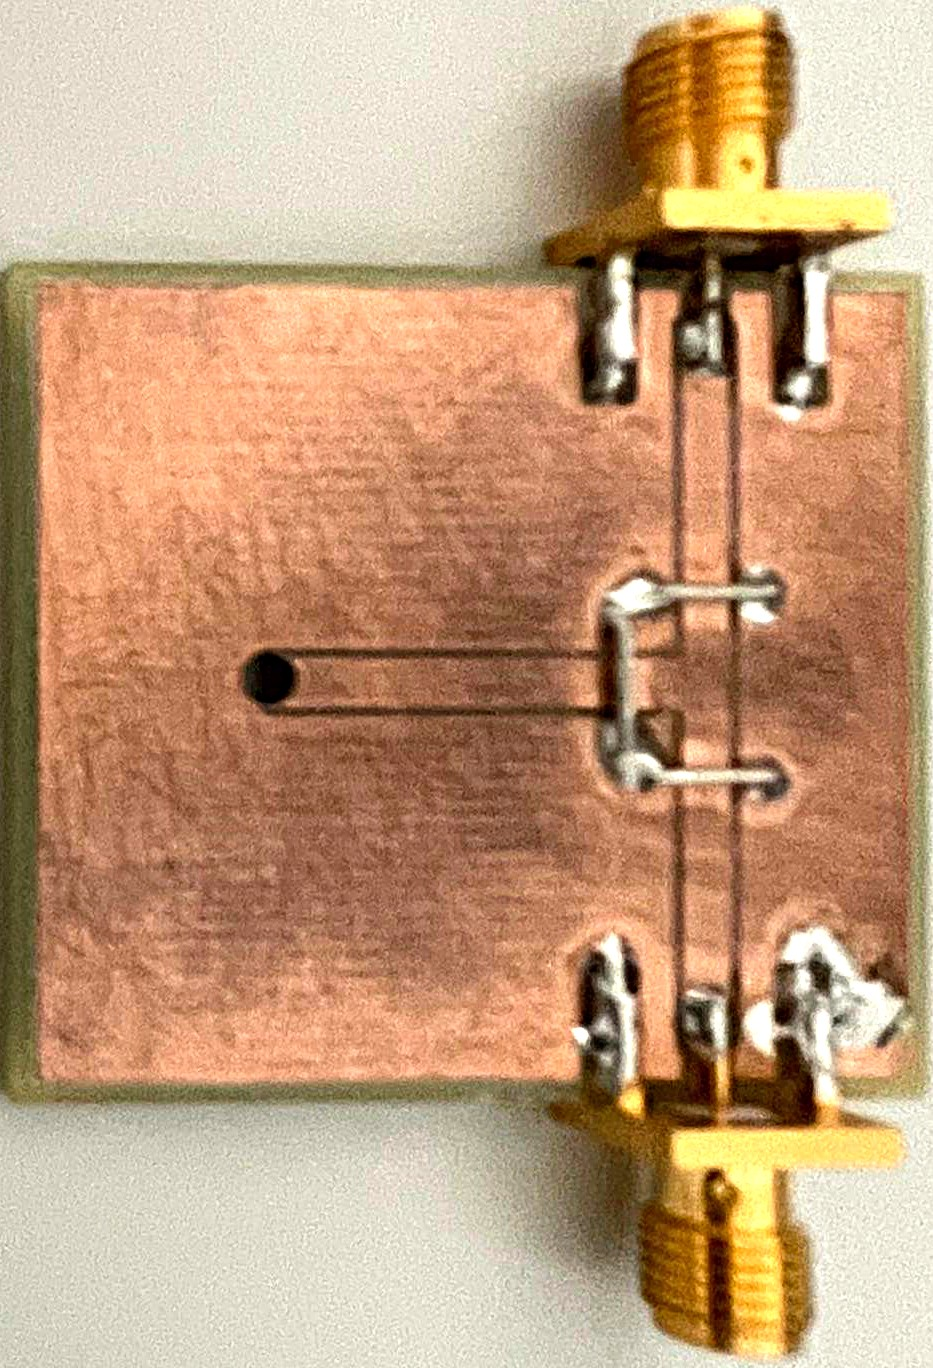
\includegraphics[scale=0.2]{images/cpw_25_rel.jpg}
    \caption{Stub coplanaire 2.5 GHz}
    \label{fig:cpw_25_rel}
\end{figure}

\newpage
\begin{figure}[h]
    \centering
    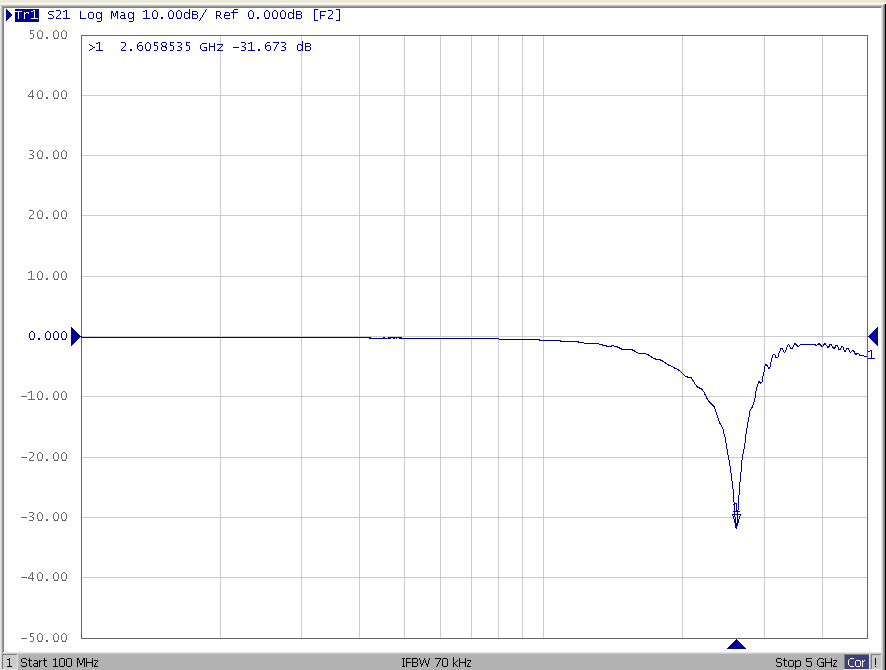
\includegraphics[scale=0.4]{images/cpw_25_mes.png}
    \caption{Réponse mesurée avec et sans jet d'eau}
    \label{fig:cpw_25_mes}
\end{figure}

\newpage
\subsubsection{Demi onde coplanaire 2.5 GHz}
Le dernier capteur mis en œuvre dans ce travail est donc un résonateur demi onde. Ce choix a été fait car contrairement à ces prédécesseurs, au lieux d'être un coupe bande c'est un passe bande, ce qui signifie que le point critique du capteur est à un puissance beaucoup plus élevée que pour les autres capteurs. Cette puissance plus élevée pourrait permettre de mesurer une plus faible variation de la puissance à la fréquence centrale du résonateur. 

\vspace{0.5cm}
Le second point est d'adapter la ligne à une impédance de 120 ohm au lieu de 50. Cela permet d'avoir des gap plus grands entre la ligne et la masse et par conséquent aux extrémités de la ligne résonnante. En effet, lorsque le diamètre jet est nettement inférieur à celui du trou dans lequel il passe, le couplage électromagnétique est mauvais par rapport au volume de liquide. Ce gap prévu pour être plus large devait résoudre ce problème.  

\vspace{0.5cm}
Pour commencer ce dernier a été designé et simulé sur Qucs. Le gap ligne-masse a été fixé à 3 mm et la ligne fait 1 mm de largeur. Le premier gap du résonnateur fait 1.5 mm et le second 0.3 mm. Les \textbf{figures \ref{fig:half_qucs_sch}} et \textbf{\ref{fig:half_qucs_meas}} montrent le schéma et les résultats obtenus à l'aide de Qucs. En utilisant la théorie, on peut calculer la longueur du stub à 39.90 mm.

\vspace{1cm}
\begin{figure}[h]
    \centering
    \begin{minipage}[b]{0.445\textwidth}
        \centering
        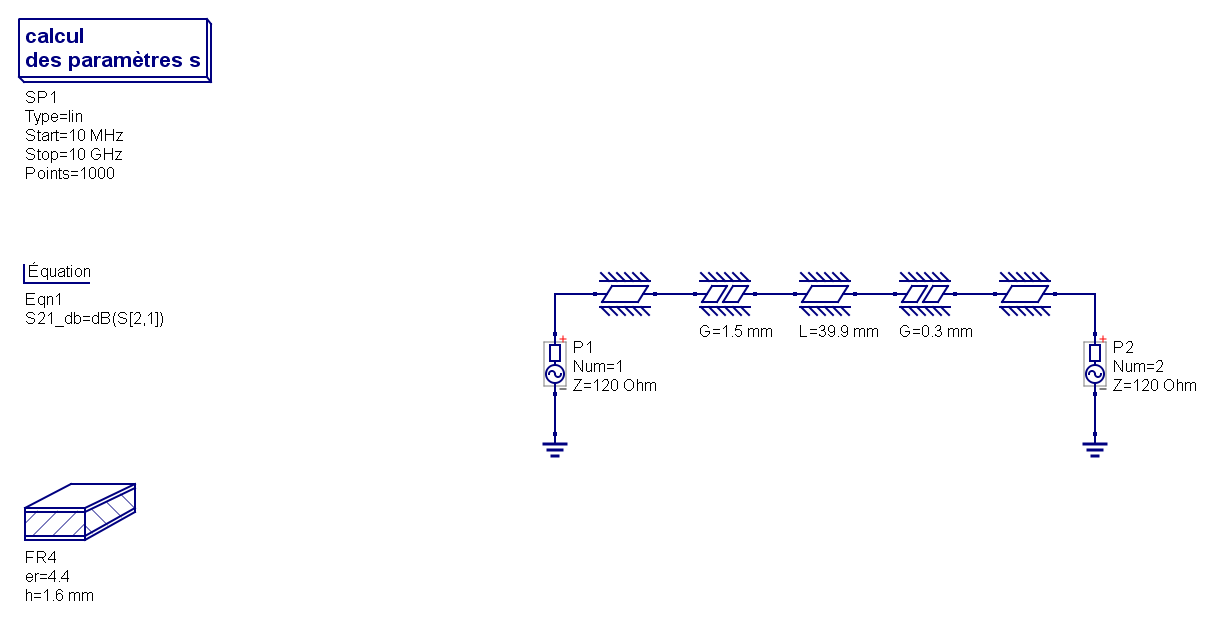
\includegraphics[width=\textwidth]{images/half_qucs_sch.png}
        \caption{\small{Schéma Qucs demi onde coplanaire 2.5 GHz}}
        \label{fig:half_qucs_sch}
    \end{minipage}
    \hspace{0.05\textwidth}
    \begin{minipage}[b]{0.45\textwidth}
        \centering
        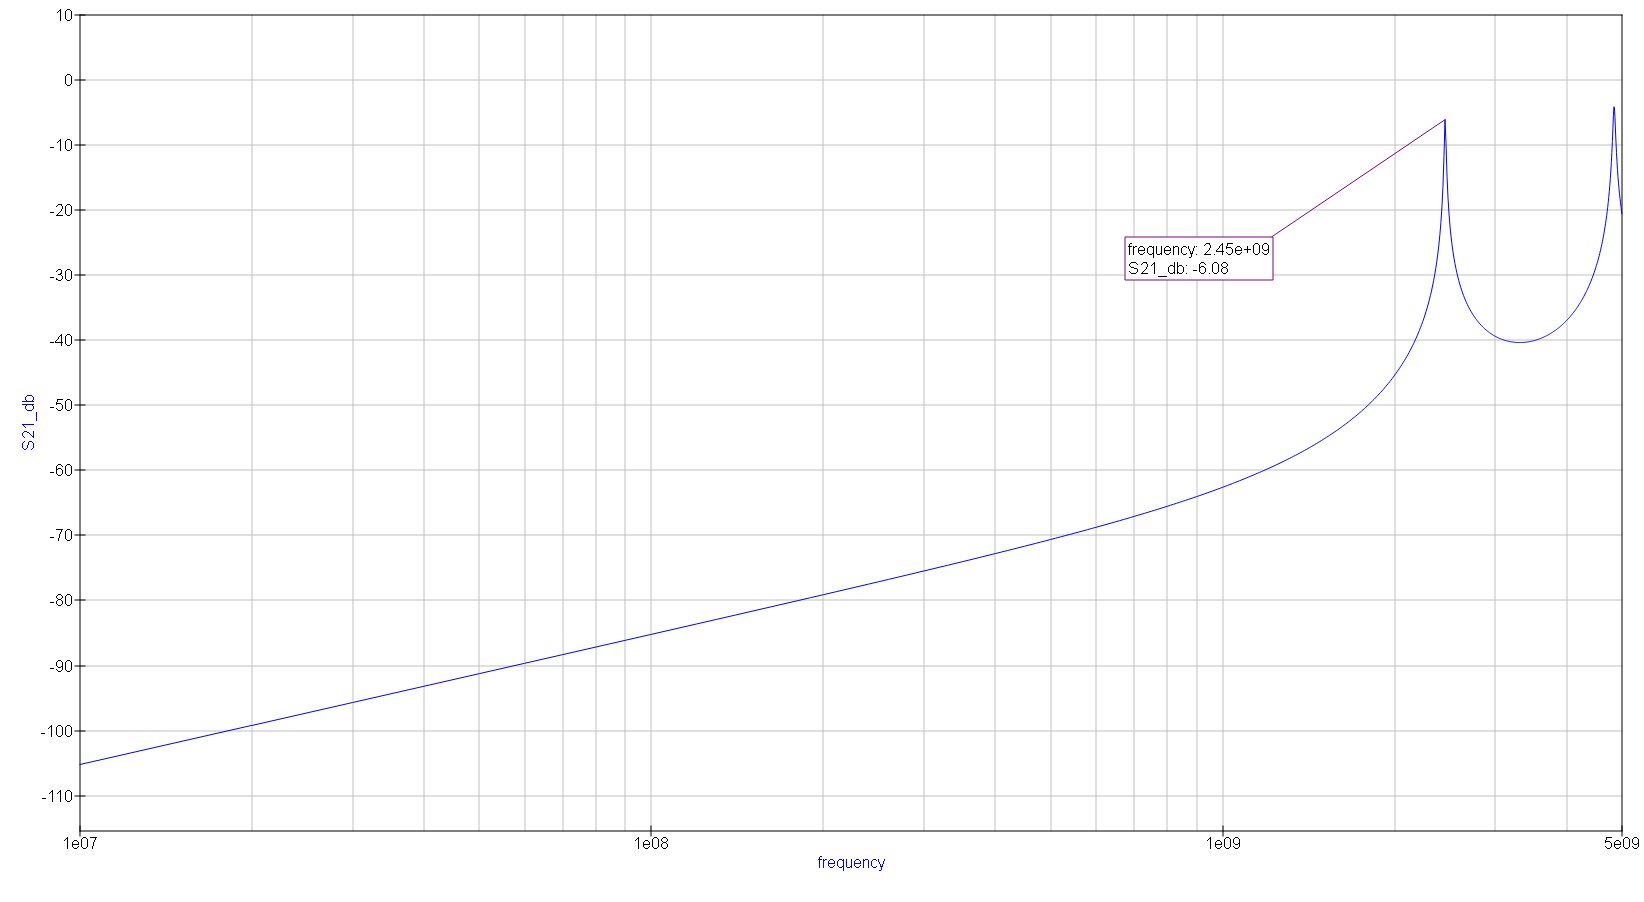
\includegraphics[width=\textwidth]{images/half_qucs_meas.png}
        \caption{\small{Résultats Qucs demi onde coplanaire 2.5 GHz}}
        \label{fig:half_qucs_meas}
    \end{minipage}
\end{figure}

\vspace{1cm}
Les résultats de Qucs donnent bel et bien une résonance à 2.5 GHz et un gain de -6dB. Ce qui est plus élevé que les -30dB des capteurs précédents. 

\newpage
La seconde étape est de simuler ce capteur du HFSS, avec et sans eau. Un design similaire à celui simulé sur Qucs a été réalisé avec la longueur du résonateur qui varie légèrement et qui induit une légère variation de la fréquence. Ce design est visible à la \textbf{figure \ref{fig:hfsshalf_24}}. On peut y voir la colonne d'eau comme pour le capteur précédent, et pour les mêmes raisons, le jet d'eau a un diamètre de 1 mm au lieux des 150 microns.   

\vspace{1cm}
\begin{figure}[h]
    \centering
    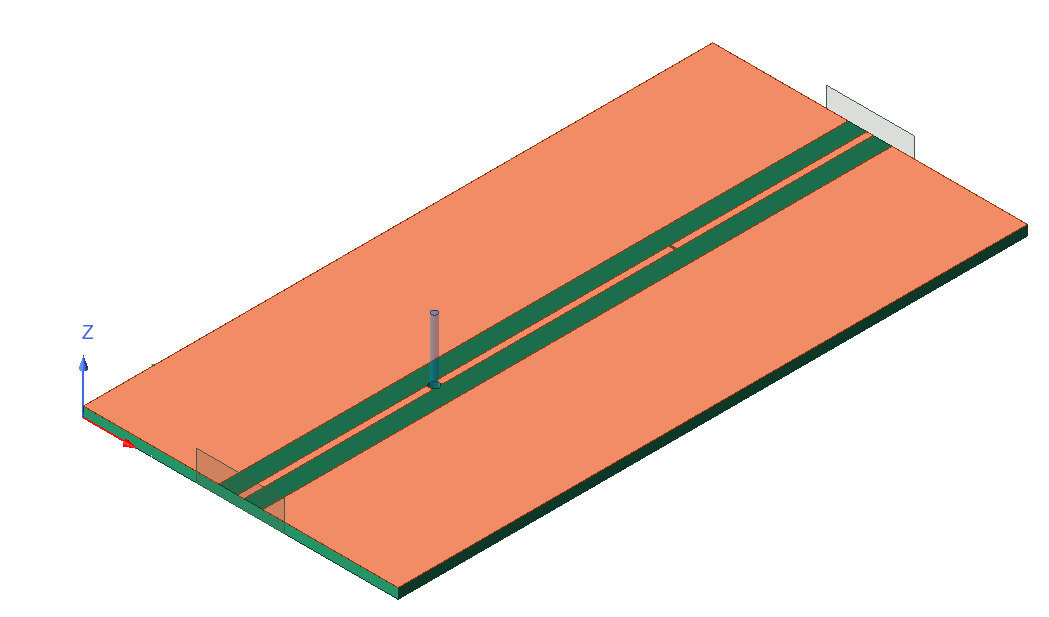
\includegraphics[scale=0.3]{images/hfsshalf_24.png}
    \caption{Demi onde coplanaire 2.5 GHz sur Ansys HFSS}
    \label{fig:hfsshalf_24}
\end{figure}

Les réponse en fréquence du design avec et sans le jet d'eau sont données aux \textbf{figures \ref{fig:hfss_sansEau}} et \textbf{\ref{fig:hfss_avecEau}}. On peut constater que la fréquence de résonance varie peu mais le gain passe de -9.9dB sans eau à -2.29dB lorsque le jet est présent. 

\vspace{1cm}
\begin{figure}[h]
    \centering
    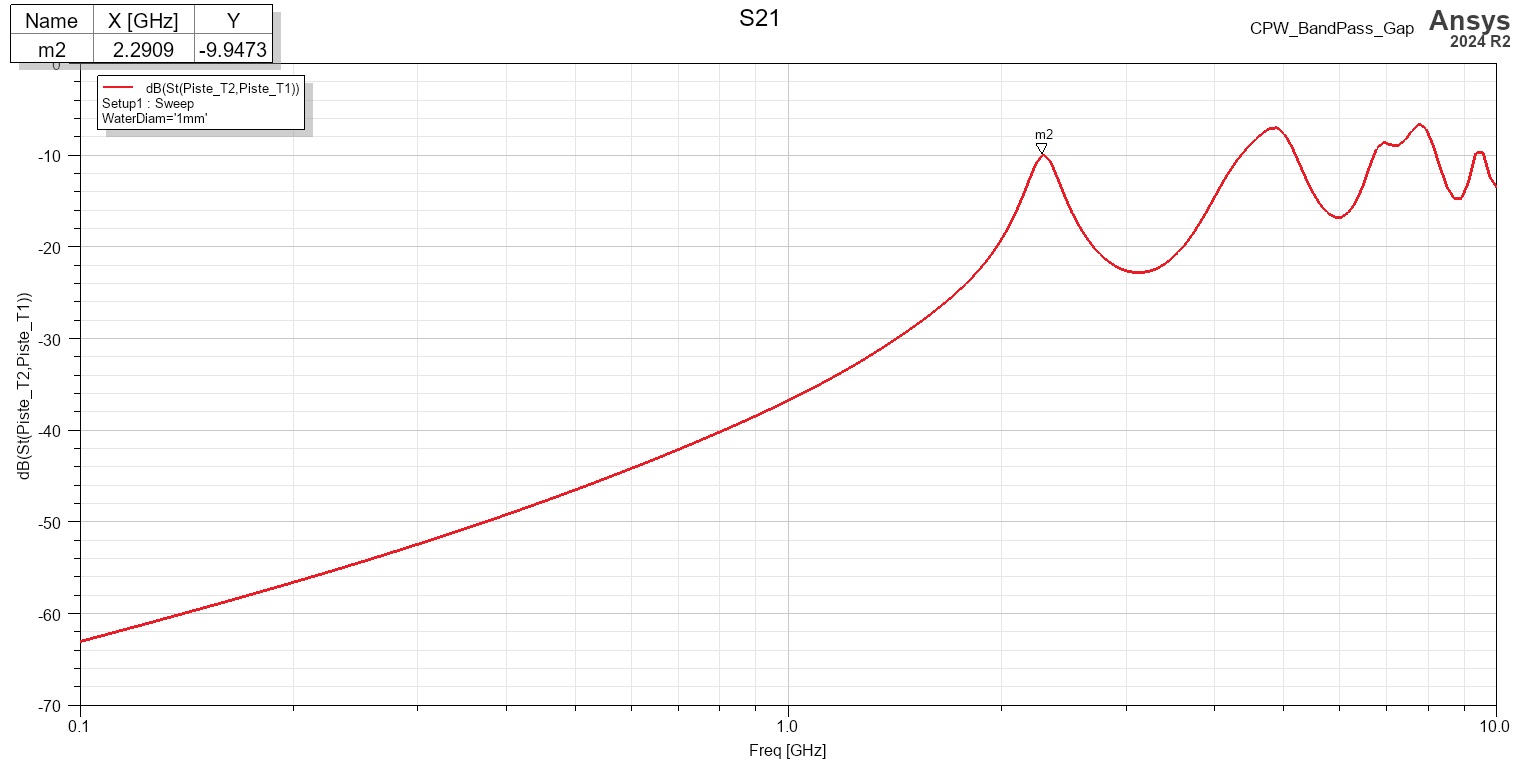
\includegraphics[scale=0.25]{images/hfss_sansEau.png}
    \caption{Réponse demi onde coplanaire sans eau}
    \label{fig:hfss_sansEau}
\end{figure}

\newpage
\begin{figure}[h]
    \centering
    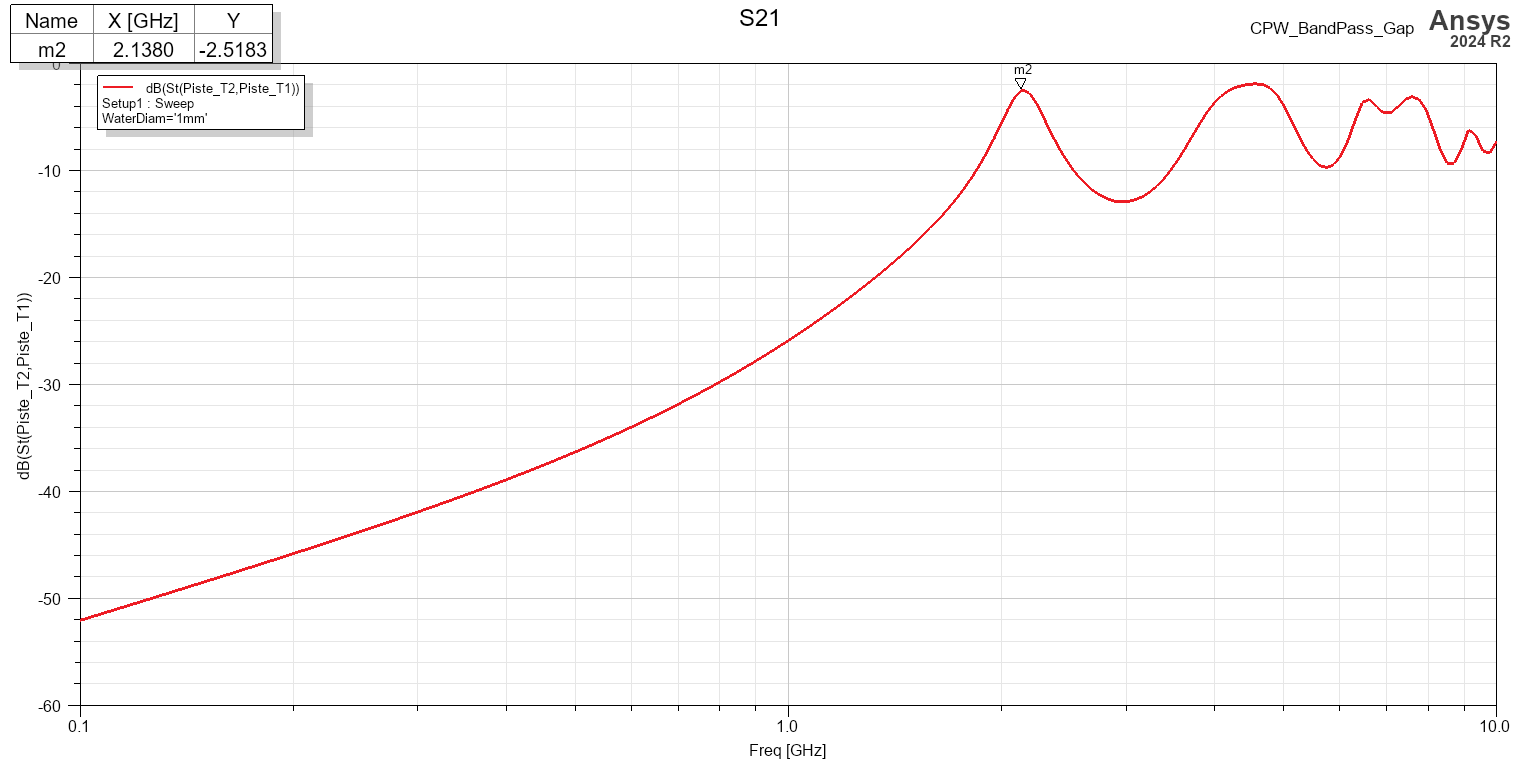
\includegraphics[scale=0.25]{images/hfss_avecEau.png}
    \caption{Réponse demi onde coplanaire avec eau}
    \label{fig:hfss_avecEau}
\end{figure}

Malgré des simulationd prometteuses avec HFSS, en cas réel avec un jet de 0.15 mm aucune différence n'est mesurable.
\vspace{1cm}
\begin{figure}[h]
    \centering
    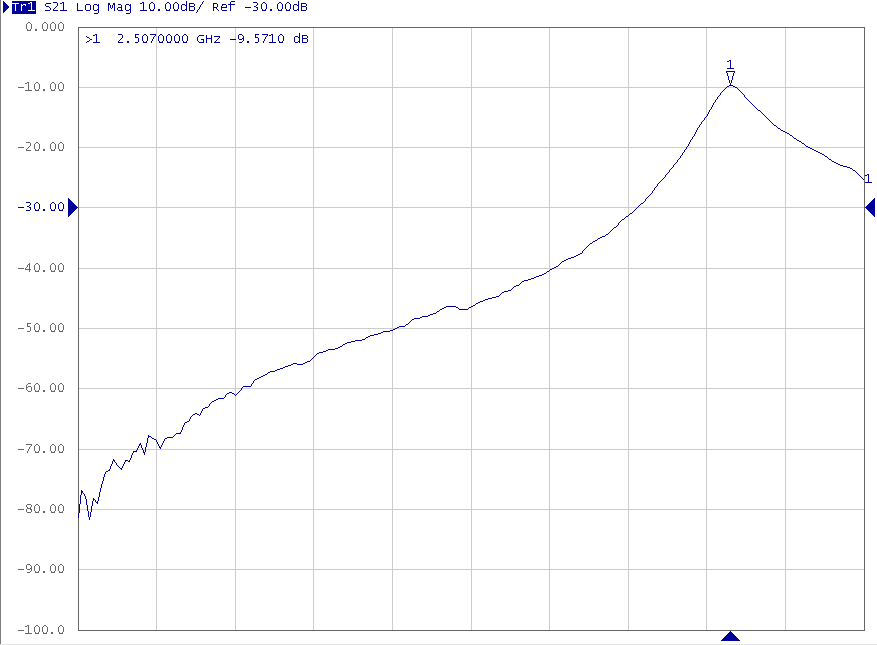
\includegraphics[scale=0.4]{images/half_24_trou.PNG}
    \caption{Réponse du demi onde coplanaire 2.5 GHz}
    \label{fig:half_24_trou}
\end{figure}

\newpage
\section{Électronique}

Afin d'adapter le système de mesure à une utilisation embarquée, deux modules compatibles mikroBus ont été réalisés. Le premier permet d'émettre un signal à une fréquence donnée grâce à un VCO. La seconde carte permet quant à elle de mesurer la puissance du signal reçu. Dans ce projet ces dernière sont monté sur la carte de développement dsPIC33CK Curiosity de chez Microchip. Elle à l'avantage de posséder 2 port mikroBus et le programmateur/débugueur se trouve directement sur la carte.  La combinaison de ces deux cartes permet de mesurer la transmission d'un réseau RF. Cette solution est extrêmement moins coûteuse et spacieuse qu'un VNA mais aussi extrêmement moins précise, mais l'utilisation n'est pas du tout la même.

\vspace{0.5cm}
Afin de simplifier l'utilisation du système, une petite interface utilisateur a été développée. Elle possède pour l'instant seulement deux modes mais c'est suffisant pour démontrer le potentiel. 

\subsection{Émetteur RF}

La première carte mise au point est celle de l'émetteur. La carte montée est visible à la \textbf{figure \ref{fig:rf_emit}}. Son fonctionnement est expliqué à la suite de son schéma bloc en \textbf{figure \ref{fig:rf_bloc}}.

\vspace{1cm}
\begin{figure}[h]
    \centering
    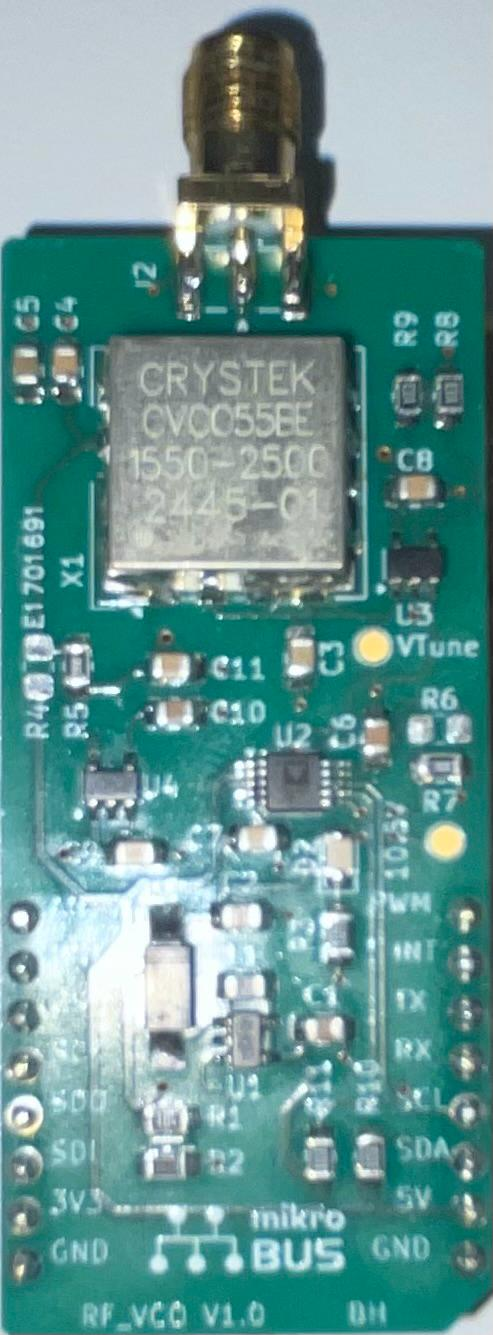
\includegraphics[scale=0.3, angle = -90]{images/rf_emit.jpeg}
    \caption{Émetteur RF}
    \label{fig:rf_emit}
\end{figure}

\newpage
\vspace{1cm}
\begin{figure}[h]
    \centering
    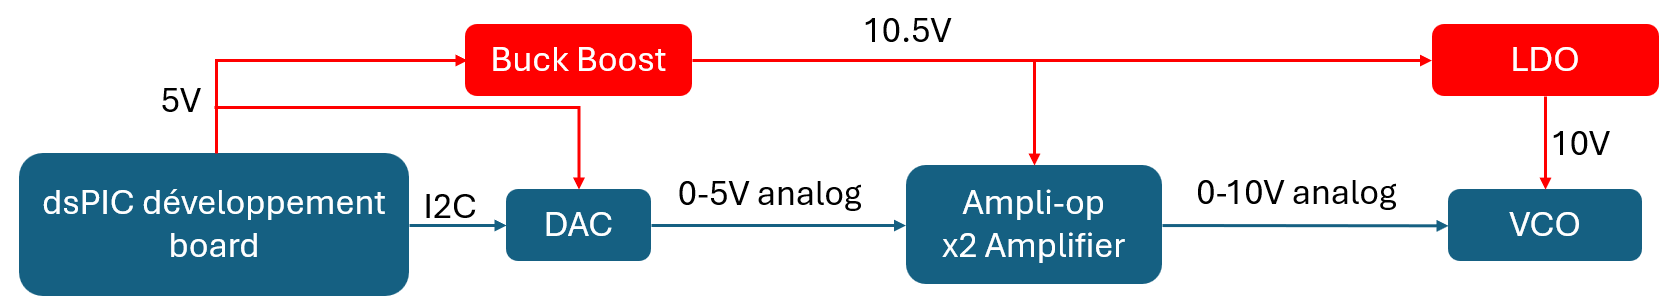
\includegraphics[scale=0.35]{images/rf_bloc.png}
    \caption{Schéma bloc Émetteur RF}
    \label{fig:rf_bloc}
\end{figure}

Le module émetteur reçois les ordres du microcontrôleur via un bus I2C, il permet de contrôler directement un DAC qui permet d'avoir une tension entre 0 et 5 V. Le VCO est contrôler en tension avec une entrée allant de 0 à 10 V. Un ampli-op ,configuré pour un gain de deux, permet d'atteindre la tension nécessaire pour le contrôle du VCO. Pour finir, un buck boost permet d'augmenter la tension un peu au dessus de 10 V pour alimenter l'ampli-op et le VCO par le biais d'un LDO pour avoir 10 V sans bruit. 

\vspace{0.5cm}
Sur le schéma électrique en annexe à la \textbf{figure \ref{fig:rf_emit_sch}}, il est possible de voir plusieurs résistances de 0 ohm, elles permettent entre autre de sélection un des bits de l'adresse I2C du DAC mais surtout de choisir l'alim du VCO car certain d'entre eux fonctionnent en 5 V. Dans ce cas il suffit de modifier les résistances de l'ampli-op pour avoir un gain de 1.

\vspace{0.5cm}
\textbf{Caractéristiques de l'émetteur :}\\
- Fréquence : 1550 MHz - 2500 MHz\\
- Puissance : compris entre 3 dBm et 9 dBm\\
- Impédance de charge : 50$\Omega$

\vspace{0.5cm}
Une mesure a été faite liant la valeur chargée dans le DAC 12 bits à la fréquence de sortie. Cela a permis par régression de calibrer ce dernier.  

\vspace{0.5cm}
\begin{figure}[h]
    \centering
    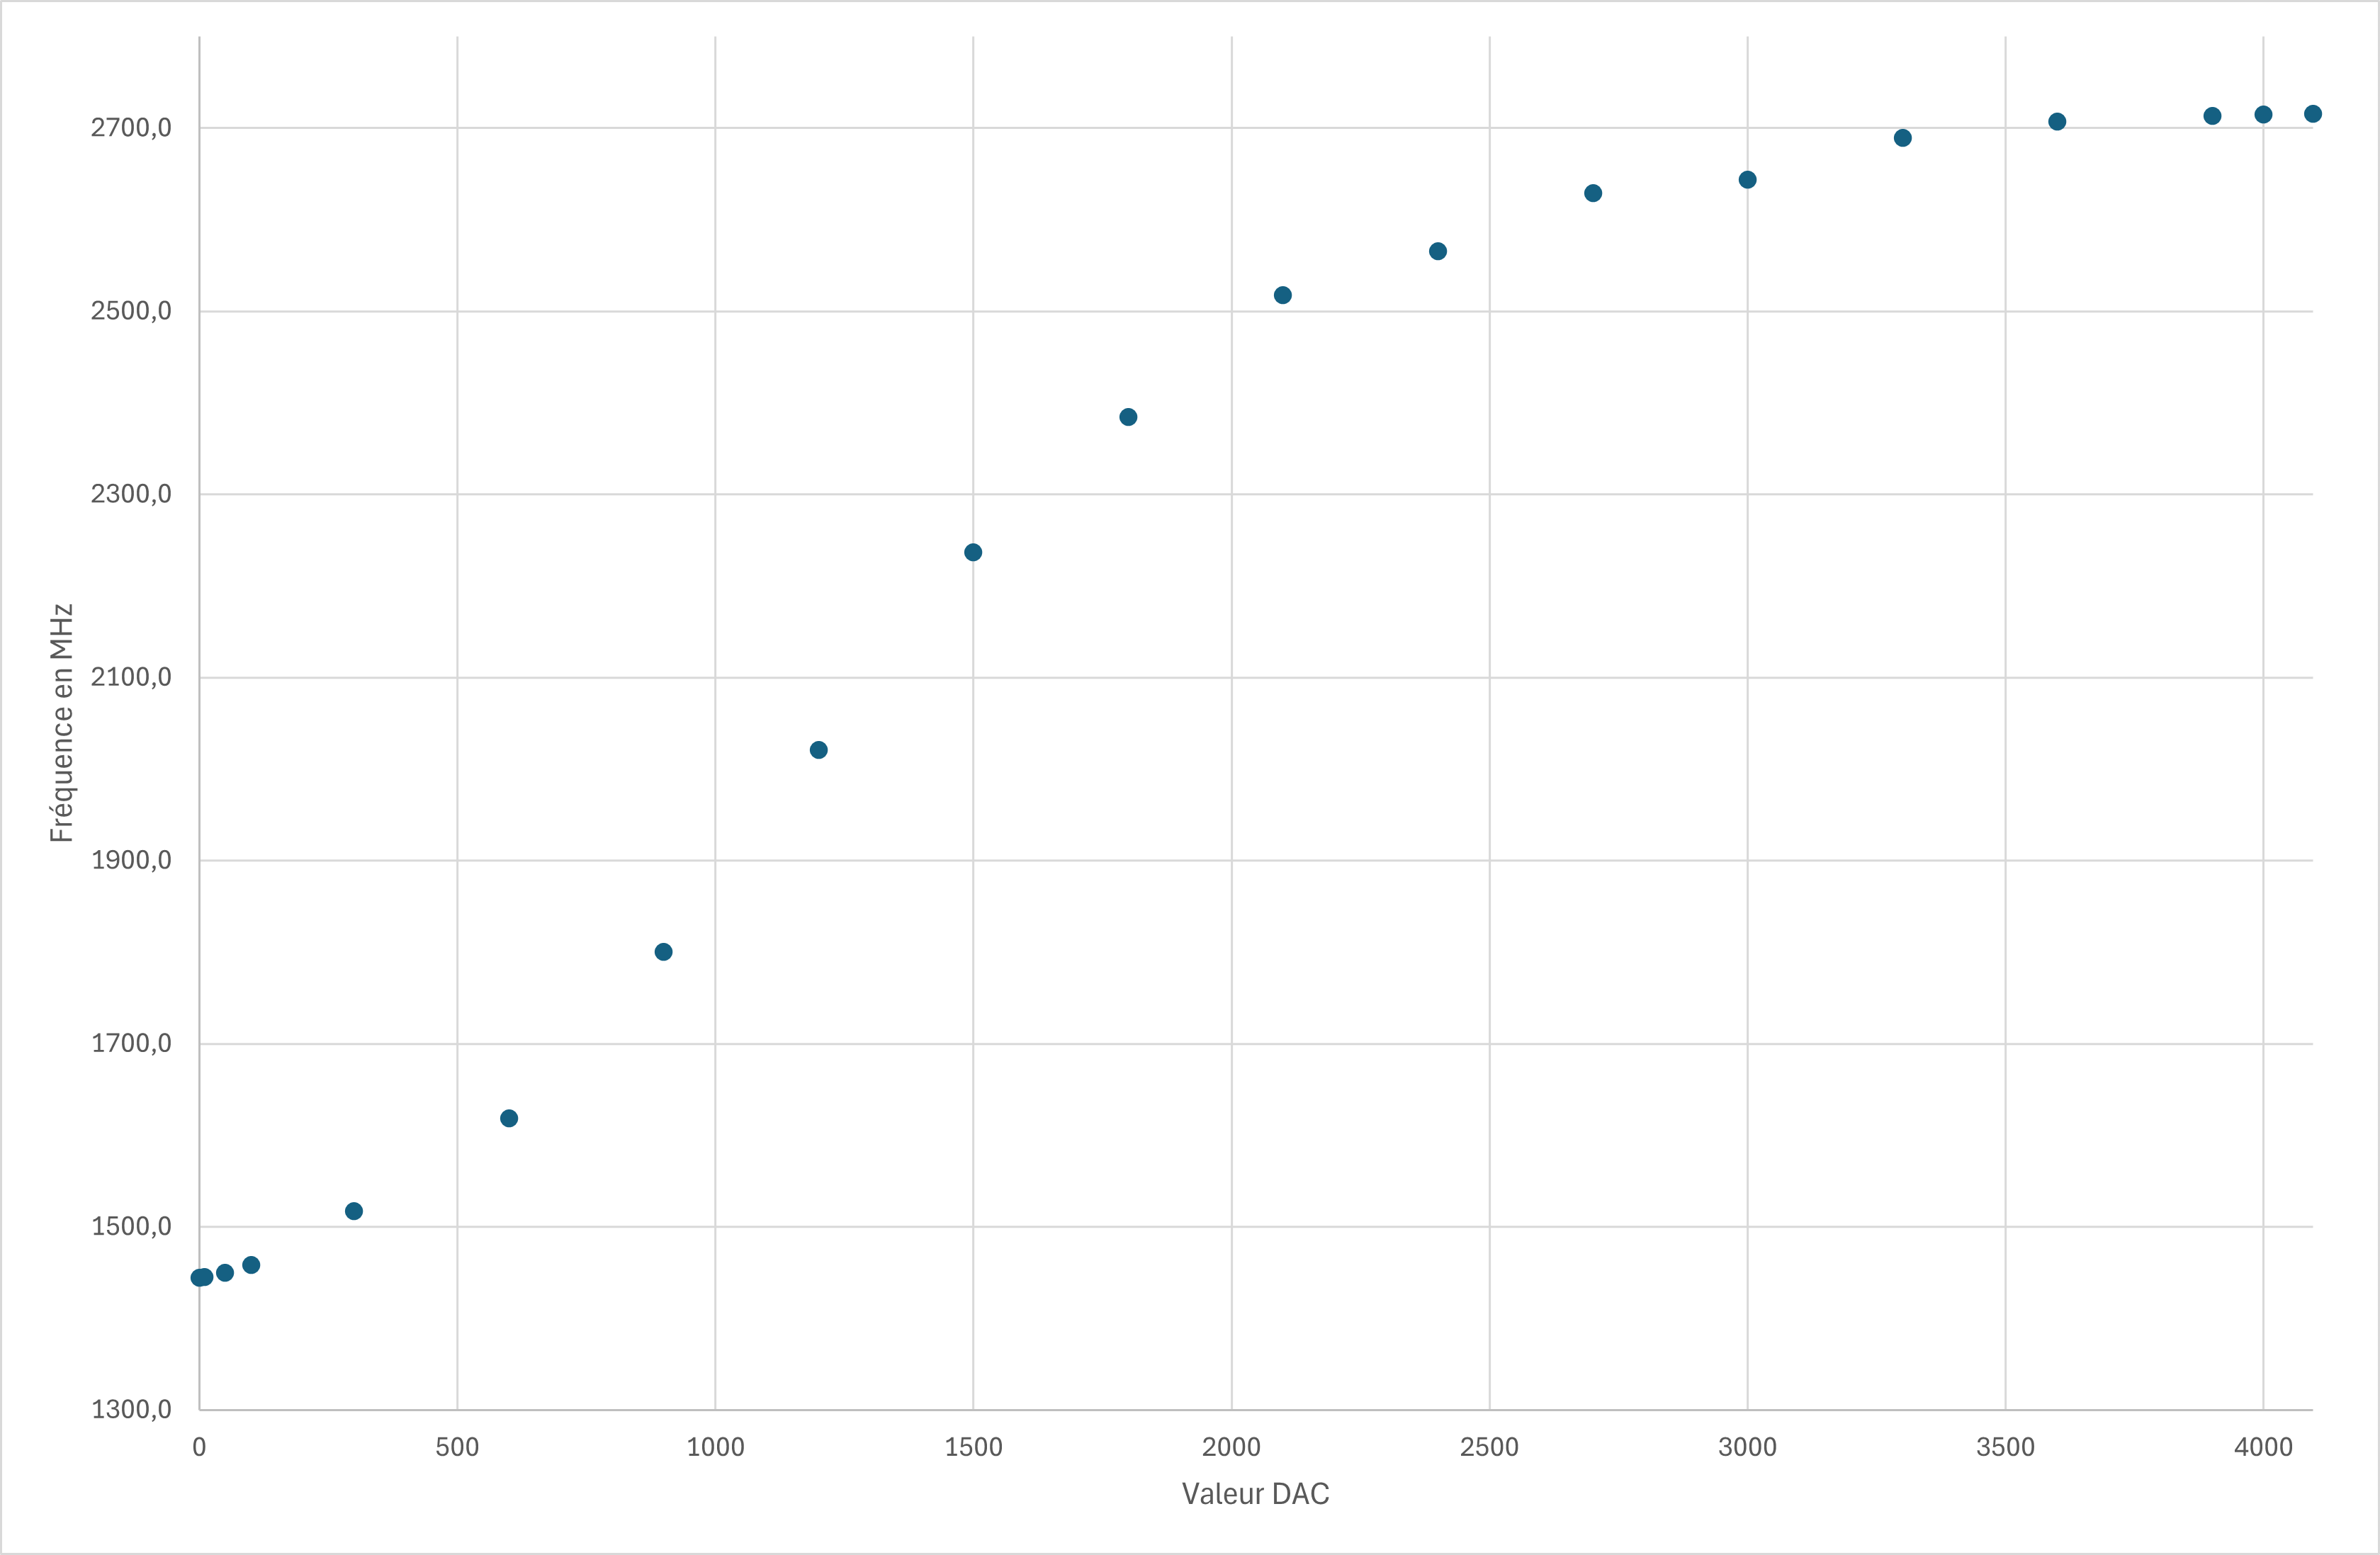
\includegraphics[scale=0.4]{images/mes_emit.png}
    \caption{Fréquence de sortie en fonction des valeurs du DAC}
    \label{fig:mes_emit}
\end{figure}

\newpage
\subsection{Récepteur RF}
La seconde carte permet de mesurer la puissance d'un signal RF. Elle est basée sur un LTC5582, c'est un chip de chez AnalogDevice qui permet de réaliser ce genre de mesures. Ce chip possède une sortie analogique qui varie entre 0 et 3V3 en fonction de la puissance du signal d'entré. La carte monté du récepteur se trouve en \textbf{figure \ref{fig:rf_recv}}.

\vspace{0.5cm}
\begin{figure}[h]
    \centering
    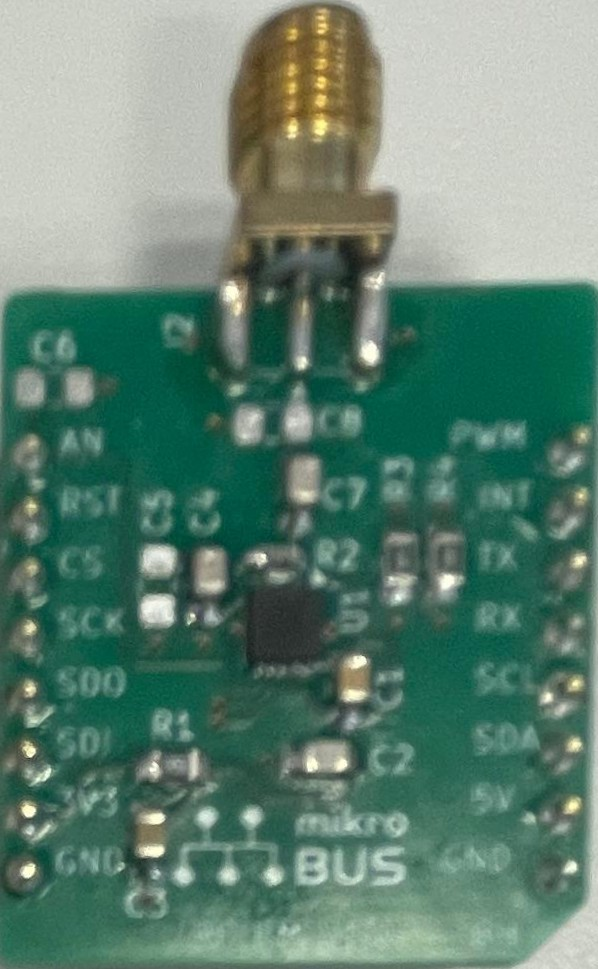
\includegraphics[scale=0.3, angle = -90]{images/rf_recv.jpg}
    \caption{Récepteur RF}
    \label{fig:rf_recv}
\end{figure}

\vspace{0.5cm}
    Le fonctionnement de cette carte est plus simple que pour la partie émetteur, en effet, elle contient uniquement le LTC5582, sur lequel arrive l'entrée RF et la sortie analogique allant dans un ADC du dsPIC.

\vspace{0.5cm}
La réponse de la carte a été mesurée et ce trouve en \textbf{figure \ref{fig:rf_recv_meas}}. Cette réponse est bien linéaire pour des fréquences basses commence déjà à être problématique à 2.5 GHz. Le LTC5582 permet de mesurer la puissance des signaux jusqu’à 10 GHz. Cette problématique provient certainement du fait que l'adaptation d’impédance de la ligne RF allant au chip est mauvaise. Malgré ces conditions le système est calibrée pour 2.5 GHz.

\begin{figure}[h]
    \centering
    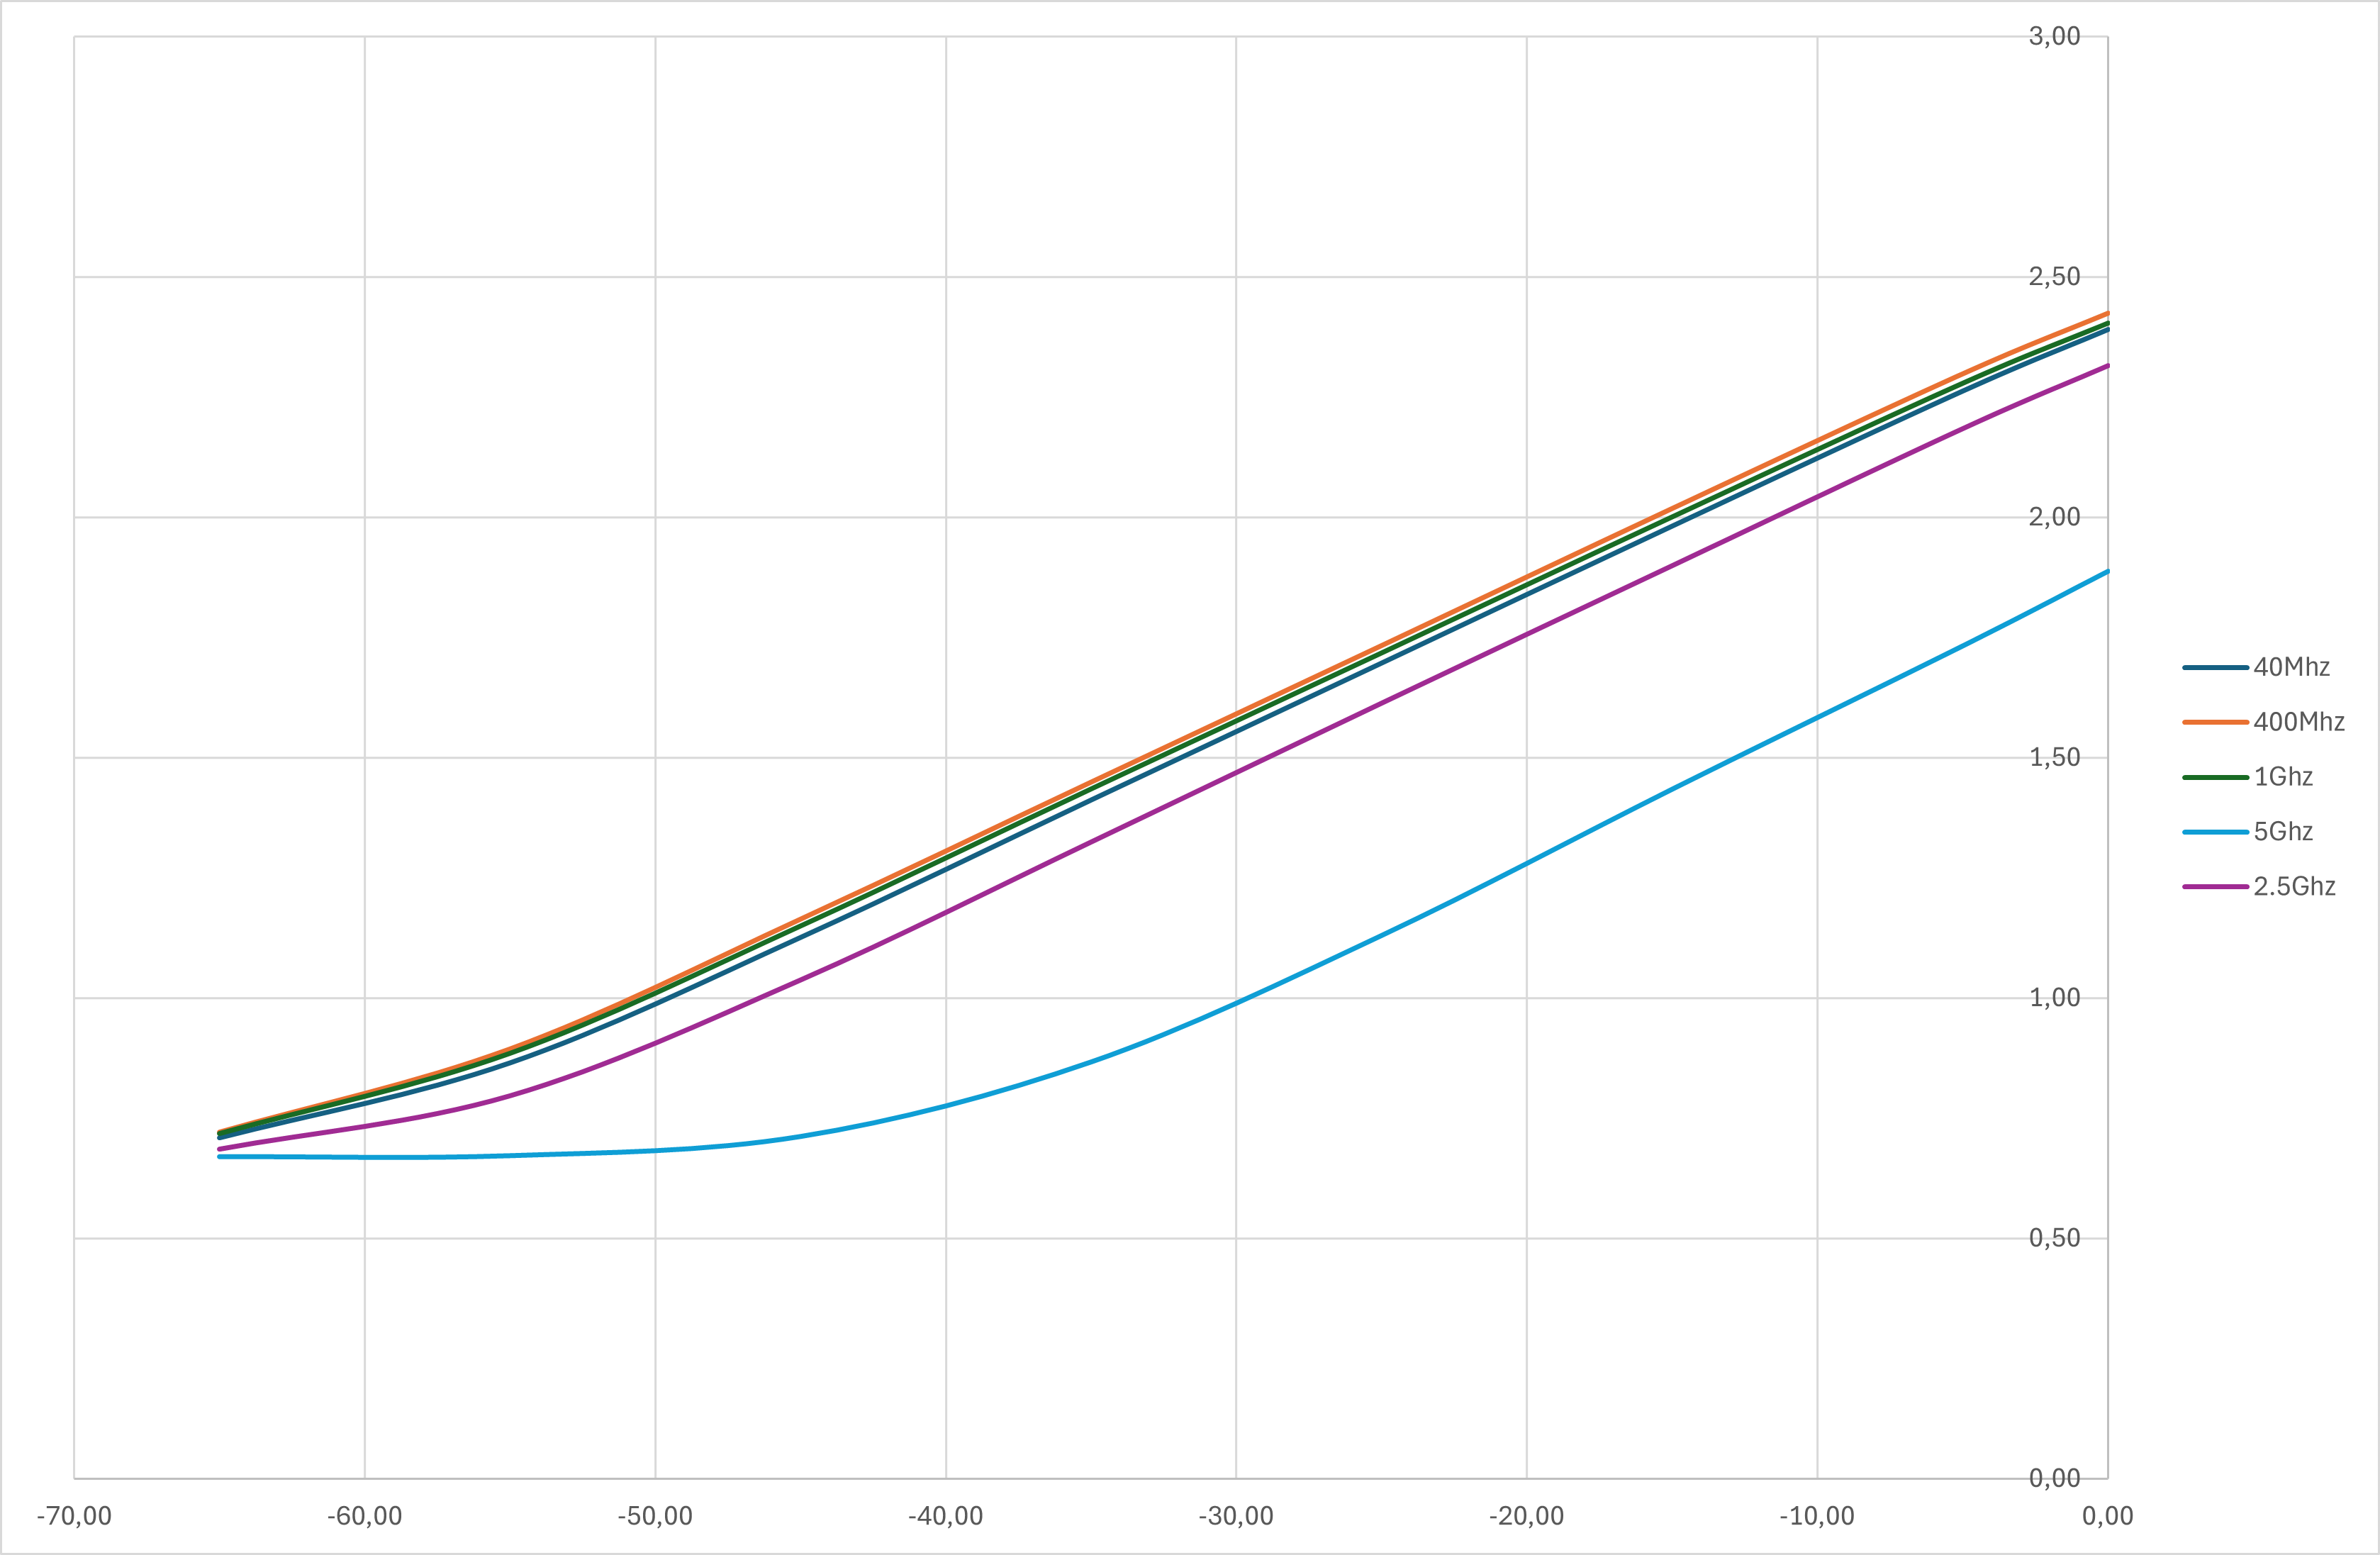
\includegraphics[scale=0.4]{images/rf_recv_meas.png}
    \caption{Réponse du récepteur RF}
    \label{fig:rf_recv_meas}
\end{figure}

\newpage
La mesure des réflexions a donc été faite à l'aide du VNA. Elle se trouve en \textbf{figure \ref{fig:rf_recv_vna}}. On voit bel et bien que, passé 1 GHz, les réflexions augmentent rapidement jusqu'à -5 dB. 

\begin{figure}[h]
    \centering
    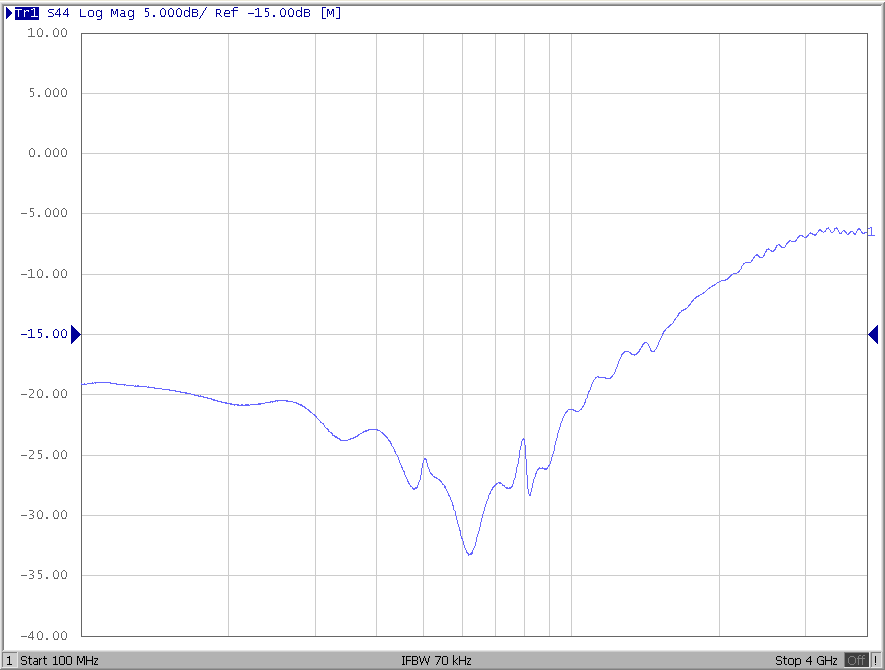
\includegraphics[scale=0.4]{images/rf_recv_vna.png}
    \caption{Réflexions du récepteur RF}
    \label{fig:rf_recv_vna}
\end{figure}

\vspace{0.5cm}
La ligne allant du connecteur SMA au chip est une ligne microruban, elle fait une largeur de 0.68 mm. La piste concernée est celle présentée par la \textbf{figure \ref{fig:piste_recv}}. D'après la théorie, la ligne microruban sur PCB de 1.6 mm de haut doit faire 3 mm afin d'avoir une impédance de 50 ohm, je suppose avoir fait cette erreur en utilisant le calculateur de qucs et, par inattention, avoir utilisé le mauvais type le ligne. 

\begin{figure}[h]
    \centering
    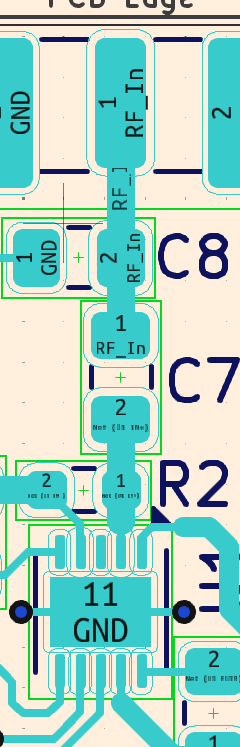
\includegraphics[scale=0.4, angle=-90]{images/piste_recv.png}
    \caption{Piste RF du récepteur}
    \label{fig:piste_recv}
\end{figure}

\newpage
Cette piste a été simulée sur Qucs afin de s'assurer de la cause du problème. Le schéma et les résultats de trouvent aux \textbf{figures \ref{fig:pistequcs}} et \textbf{\ref{fig:pistequcs_meas}}.

\vspace{0.5cm}
\begin{figure}[h]
    \centering
    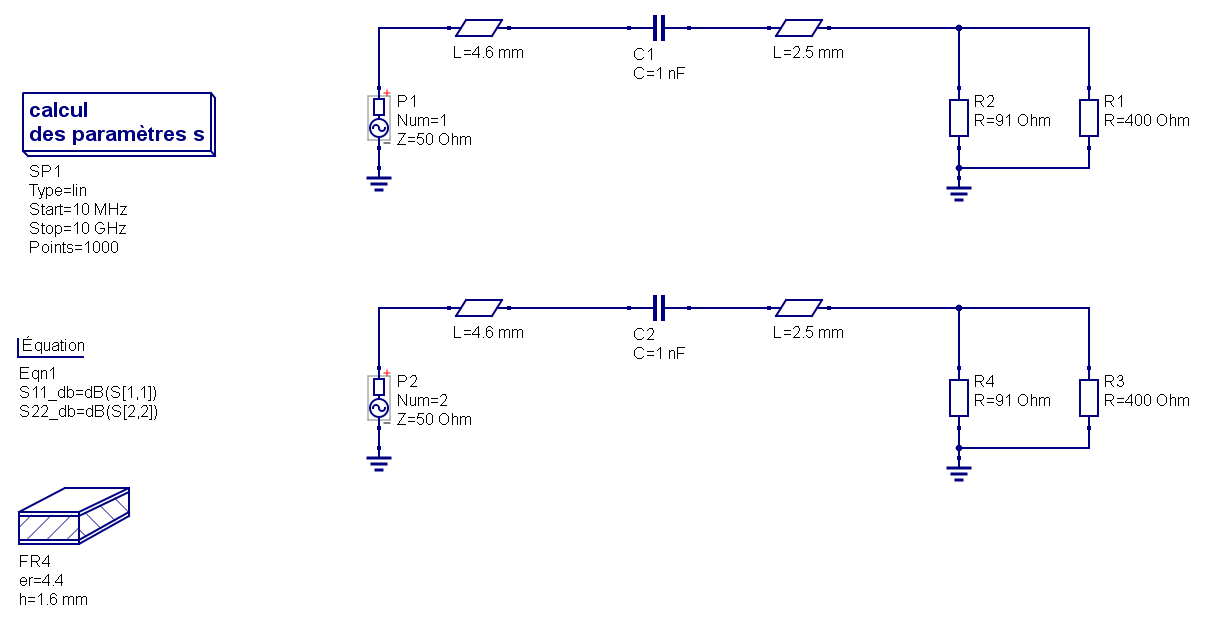
\includegraphics[scale=0.25]{images/pistequcs.png}
    \caption{Schéma de la piste sur Qucs}
    \label{fig:pistequcs}
\end{figure}

\vspace{0.5cm}
\begin{figure}[h]
    \centering
    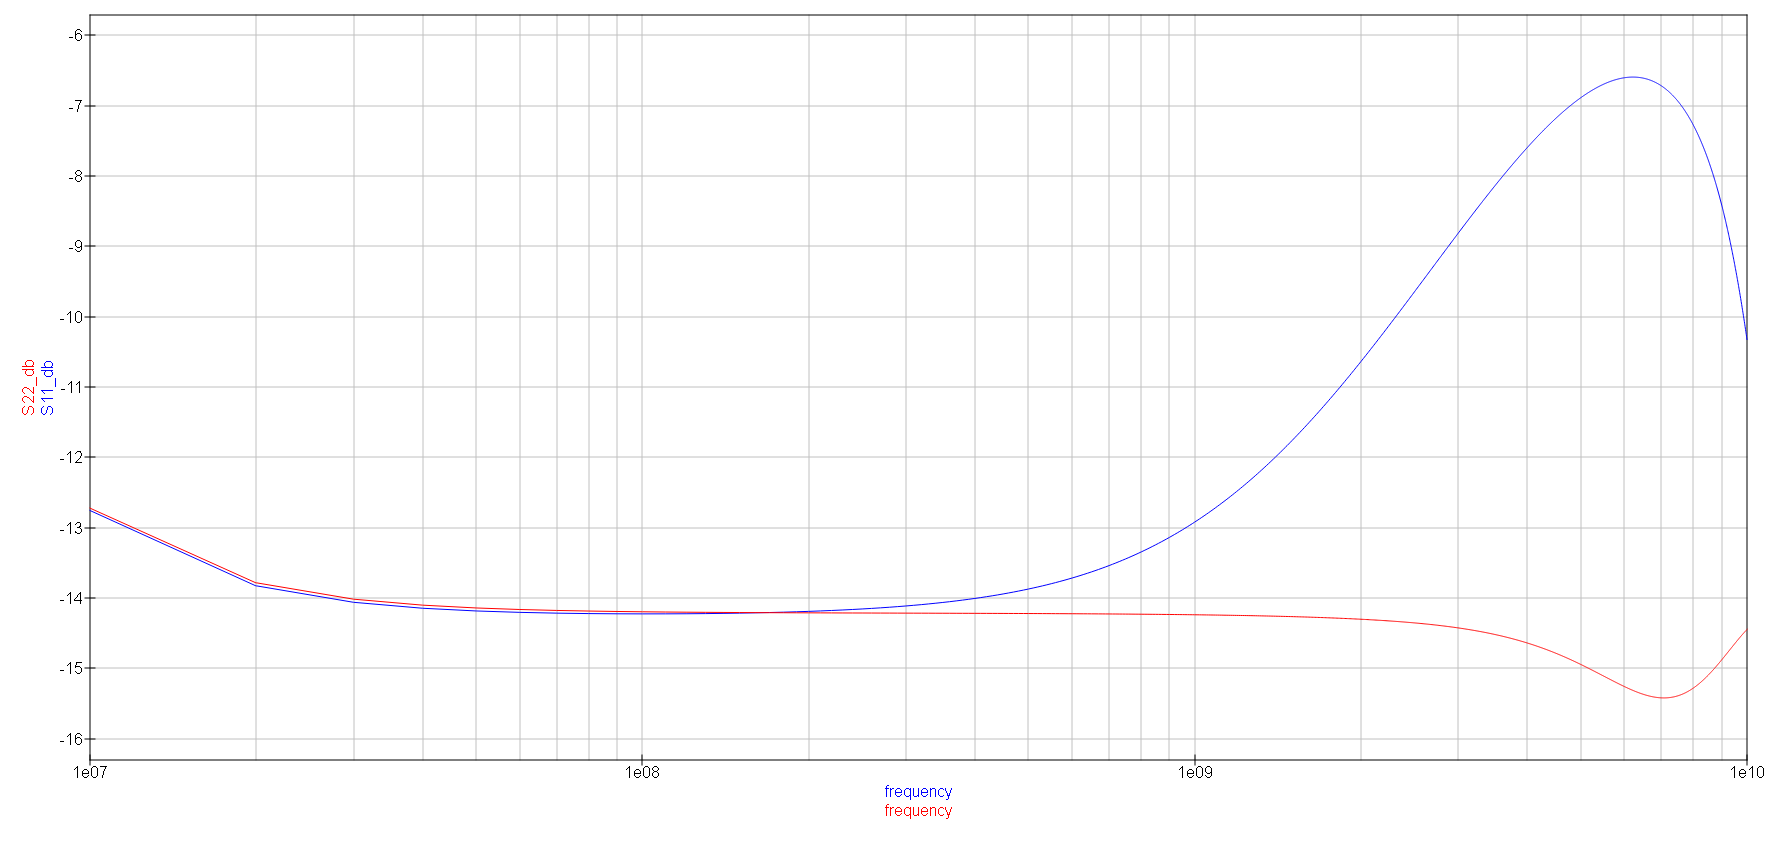
\includegraphics[scale=0.25]{images/pistequcs_meas.png}
    \caption{Résultats de la piste simulé sur Qucs}
    \label{fig:pistequcs_meas}
\end{figure}

\vspace{0.5cm}
La courbe S11 est la réflexion de la piste actuelle et la courbe S22 est la réflexion de la piste de largeur 3 mm. On retrouve clairement une courbe similaires à celles du VNA pour la piste inadaptée avec une augmentation des réflexions à 1 partir de 1 GHz. Avec la largeur de piste de 3 mm la courbe est bien meilleur et les réflexions restent à moins de -14 dB jusqu'à 10 GHz. Ces simulations semblent confirmer la provenance de l'erreur et comment améliorer le future PCB.

\newpage
\subsection{Software}
Deux softwares ont été réalisés, le programme du microcontrôleur et une interface utilisateur pour simplifier l'utilisation.

\vspace{0.5cm}
Le programme du microcontrôleur est une simple machine d'état, un état ou elle n'est pas connecté au PC, un ou elle est connecté mais en stand-by, et un dernier ou le micro met a jour la fréquence du VCO et lis la valeur du récepteur en boucle. Elle envoie les données à chaque changement au pc. 

\vspace{0.5cm}
Le programme sur pc permet d'interfacer avec le microcontrôleur, elle permet de s'y connecter, choisir la fréquence du VCO et lire la puissance du signal reçu. L'application possède un mode automatique pour faire un balayage en fréquence. Le balayage en fréquence est pour l'instant très lent mais peut être énormément amélioré. Un algorithme permet déjà cependant de ne pas surcharger la bande passante entre le pc et le microcontrôleur, cela pour ne pas empêcher le transfert de certains paquets avec plus l’importance que d'autres.

\vspace{0.5cm}
La première interface en \textbf{figure \ref{fig:dash}}, est le tableau de bord, elle permet de modifier la fréquence du VCO à la main et de lire la puissance mesurée. Les flèches haut et bas du clavier permettent d'augmenter ou diminuer la fréquence, et les chiffres 1, 2 et 3, permettent de modifier le multiplicateur entre x1, x10 et x100.

\vspace{0.5cm}
\begin{figure}[h]
    \centering
    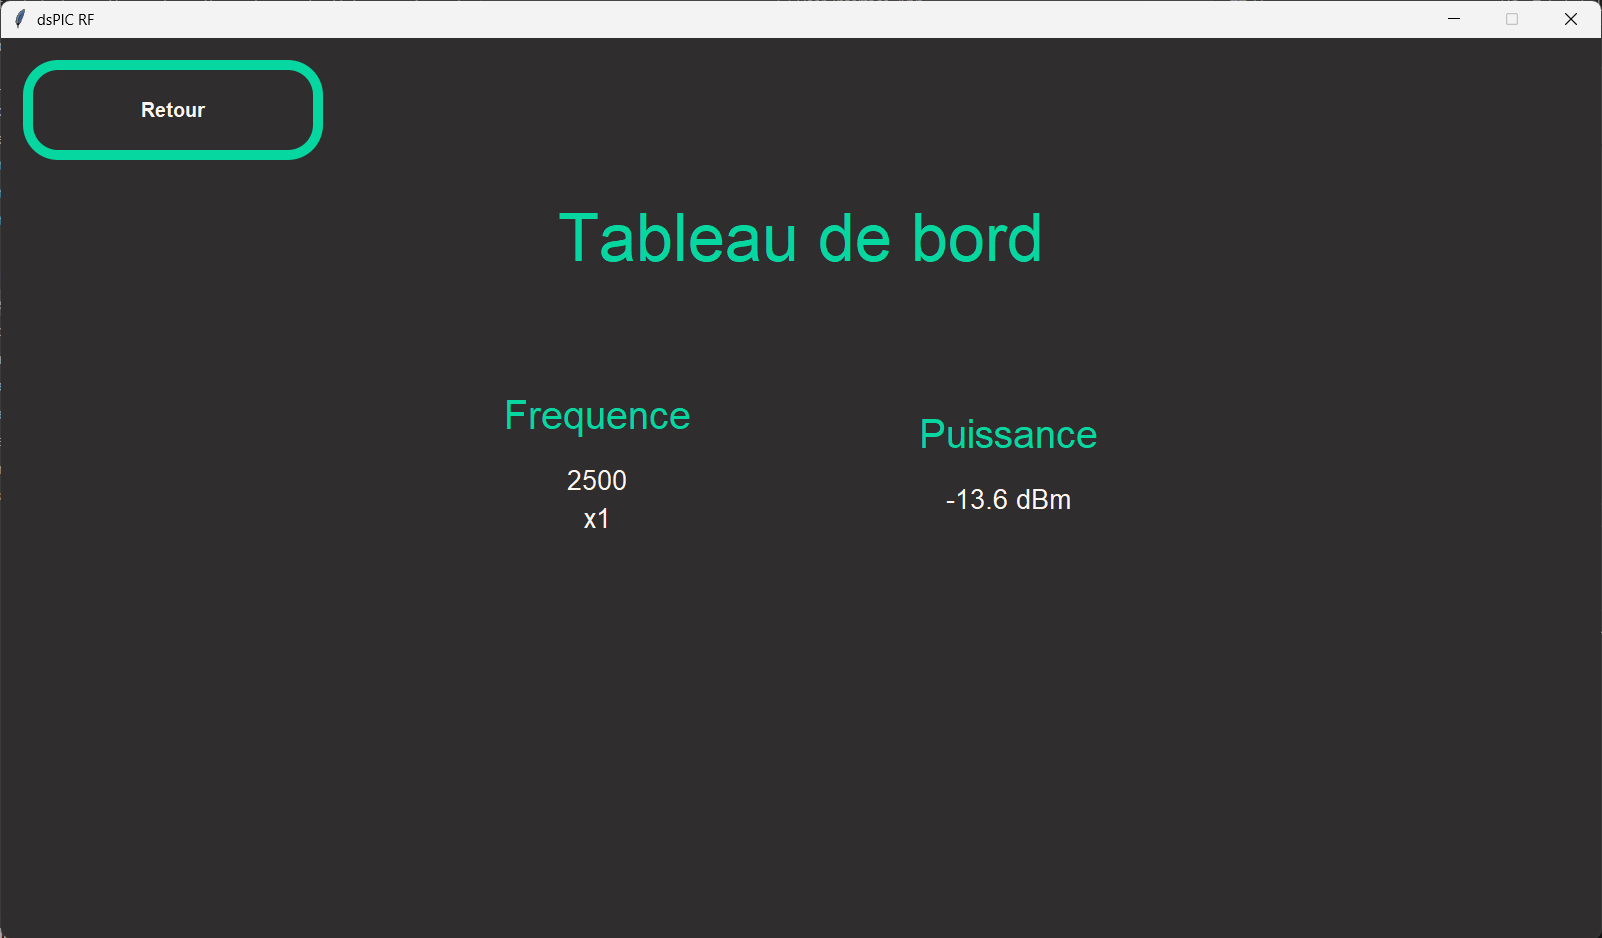
\includegraphics[scale=0.4]{images/dash.png}
    \caption{Interface Dashboard}
    \label{fig:dash}
\end{figure}

\newpage
L'autre interface est celle du balayage fréquentiel, deux mesures ont été faites. Une sur le demi onde coplanaire vu précédemment, et la seconde sur un stub microruban coupant à 2 GHz. 

\vspace{0.5cm}
\begin{figure}[h]
    \centering
    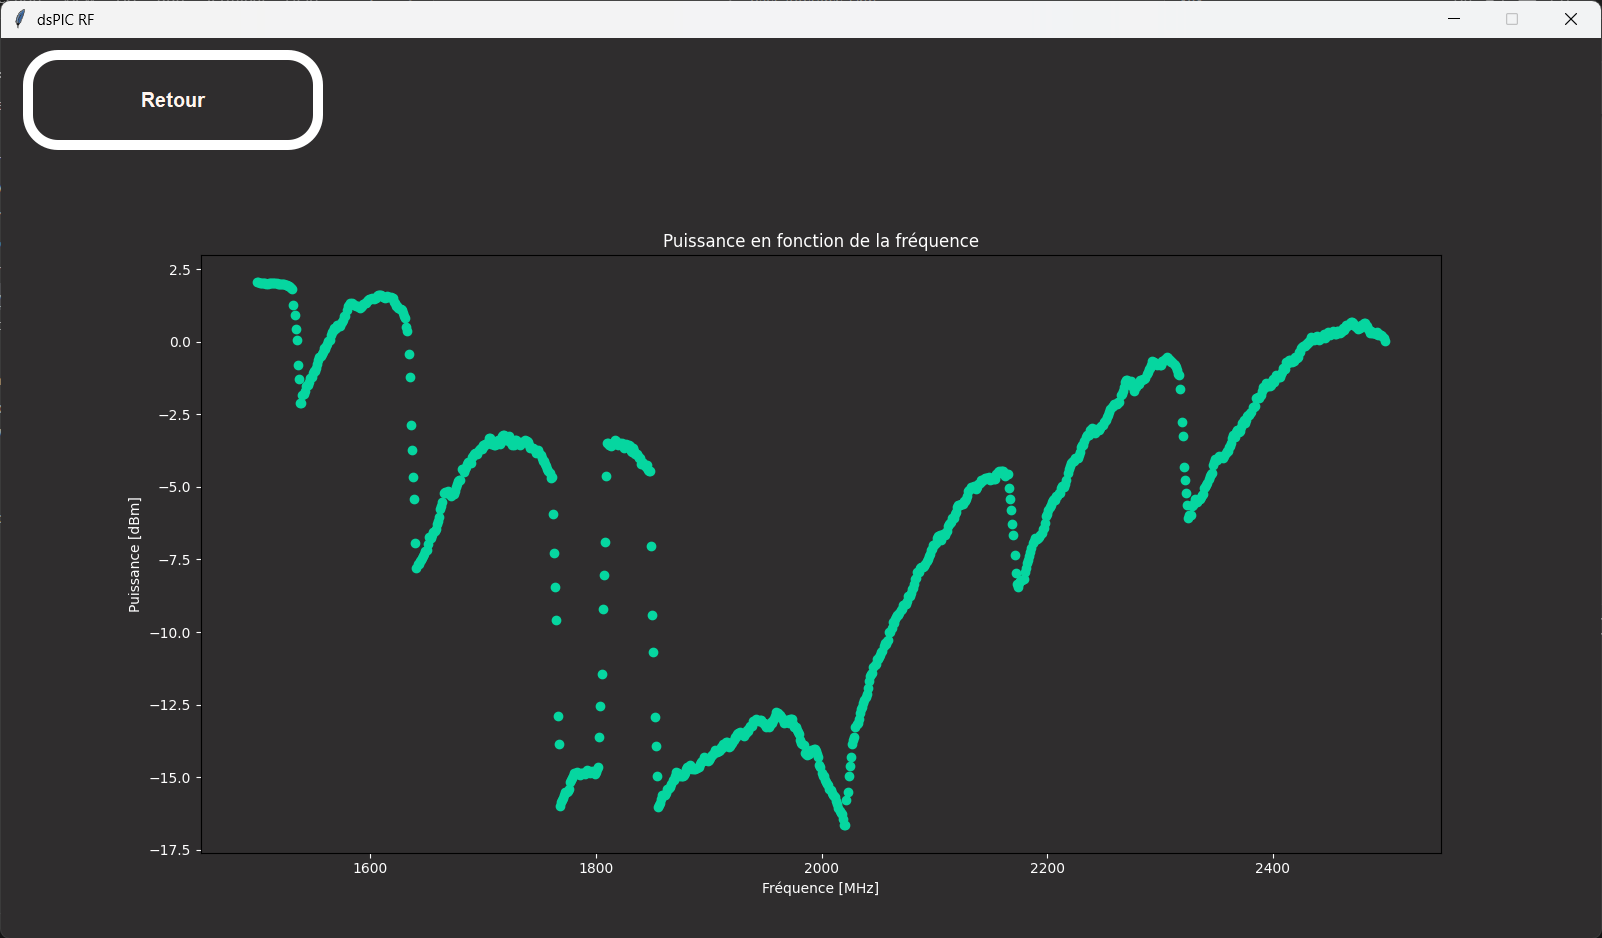
\includegraphics[scale=0.3]{images/mymeas_stub.png}
    \caption{Mesure Stub 2 GHz}
    \label{fig:mymeas_stub}
\end{figure}

\vspace{0.5cm}
\begin{figure}[h]
    \centering
    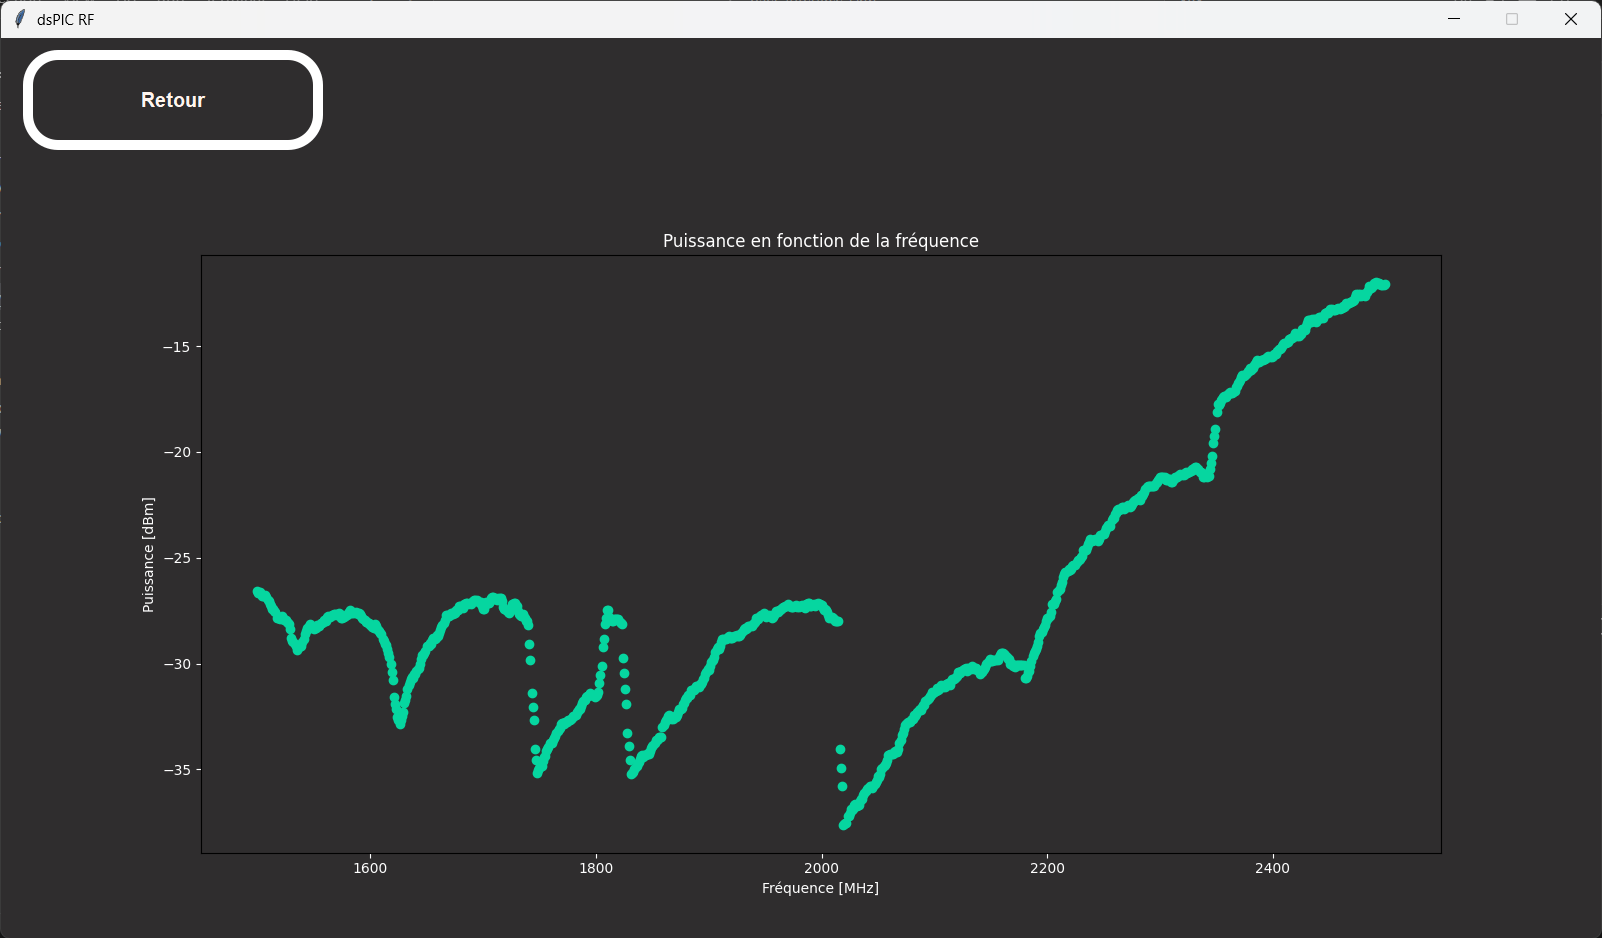
\includegraphics[scale=0.3]{images/mymeas_bandpass.png}
    \caption{Mesure demi onde 2.5 GHz}
    \label{fig:mymeas_bandpass}
\end{figure}

\vspace{0.5cm}
Ces mesures sont loin d'être parfaites, mais on peut tout de même reconnaître la réponse approximative de ces circuits, on reconnaît la forme d'entonnoir du stub, et pour le demi onde, on voit que la puissance transmise est faible à basse fréquence et augmente aux abords des 2.5 GHz. Ces mauvaises mesures sont explicables par la mauvaise adaptation de la ligne, en effet seul la mesure à 2.5 GHz est juste puisque le système est calibré pour cette dernière. Si la ligne est bien adaptée, toutes les fréquences doivent agir de la même façon et de façon linéaire. Le second point qui peut améliorer les mesures serait de pouvoir faire une calibration semblable à celle du VNA, avec des modèles de DUT bien connue.

\newpage
\section{Conclusion}
\vspace{0.5cm}
Malgré que le résultat ne soit pas celui espéré, ce travail m'a appris certaines notions, et reste une avancée, même microscopique, dans ce nouveau système de mesure de débit qui sera, je l'espère un jour, révolutionnaire.

\vspace{0.5cm}
Pour commencer, ce travail de diplôme m'a permis d’approfondir mes connaissances en électronique. En grande partie les notions de transfert d'énergie en électronique. Mais j'ai aussi eu l'occasion de mieux comprendre la polarisation des matériaux et d'où provenait les caractéristiques qui les distinguent. Il m'a également permis de mettre en œuvre de petits circuits RF simples mais surtout de les caractériser à l'aide d'un VNA en découvrant cet appareil de mesure.

\vspace{0.5cm}
Ce travail a aussi permis de mettre en avant certaines structures RF pour accomplir la tâche souhaitée, de voir leur avantage et leur inconvénient. Si de futures électroniciens reprennent le projet, j'espère que le travail fourni permettra un gain de temps notable.  

\vspace{0.5cm}
Selon moi, l'enjeu principal est de trouver une intégration à la restriction de la vanne afin de maximiser la taille du jet vis à vis du couplage électromagnétique sans pour autant que la capillarité pose problème. Un deuxième point à explorer est bien sur d'augmenter les fréquences, en effet. si les fréquences mises en jeu augmentent, les dimensions deviennent plus petites et se rapprochent de celles du jet.

\vspace{0.5cm}
Du point de vue électronique, la partie réception est à revoir pour améliorer l’adaptation d’impédance. Quant à la partie émission, ce pourrait être un plus de caractériser, en plus de la fréquence, la puissance et le facteur de qualité du signal émit pour chaque fréquence. Ces améliorations devraient permettre de gagner en précision de mesure. 

\vspace{0.5cm}
Au niveau du software, ajouter une mesure temporelle en plus de la mesure fréquentielle peut être intéressant. Du plus, beaucoup d'optimisations peuvent être faites, en commençant par utiliser la partie hardware du dsPIC pour l'I2C.

\vspace{0.5cm}
Pour finir, ce travail m'a aussi permis de me rendre compte de l’ampleur des travaux de recherche. J'ai eu l'occasion d’échanger avec des chercheurs et, quelque soit le domaine, les résultats sont rarement ceux espérés en début d'étude. Bien que cela soit très frustrant, c'est le jeu. 

\newpage
\section{Remerciements}

Je tiens à adresser, dans un premier temps, mes sincères remerciements à FAS pour avoir soumis leur problématique intéressante à HEPIA. 

\vspace{0.5cm}
Dans un second temps, je souhaite remercier grandement monsieur\\ Hervé Eusèbe pour avoir supervisé ce travail et pour le bagage intellectuel en électronique RF qu'il a su m'apporter.

\vspace{0.5cm}
Pour finir, je remercie aussi les différents professeurs de HEPIA ainsi que les assistants qui ont pu répondre à mes questions et m'aider pour différentes tâches liées à ce projet.

\vspace{12cm}
Genève, le 17 juillet 2025

\vspace{0.5cm}
Basile Hiltpold

\begin{figure}[ht]
    \hspace{1cm}
    
\includegraphics[width=0.2\linewidth]{images/signature.png}
\end{figure}

\newpage
{\Large\textbf{Références}}
\vspace{1cm}

\newcommand{\documentitem}[2]{
    \item #1 \\
    \href{#2}{\textit{Lien}} \vspace{0.2cm}
}

\begin{enumerate}[leftmargin=2cm]
    \documentitem{UIT - Règlement des radiocommunications}{https://www.itu.int/hub/publication/r-reg-rr-2024/}
    \label{ref:radio_com}

    \documentitem{Effects of humidity on sand and dust storm attenuation predictions based on 14 GHz measurement}{https://www.researchgate.net/publication/347924027_Effects_of_humidity_on_sand_and_dust_storm_attenuation_predictions_based_on_14_GHz_measurement}
    \label{ref:air_storm}

    \documentitem{Conféderation Suisse - Humidité de l'air}{https://www.meteosuisse.admin.ch/meteo/meteo-et-climat-de-a-a-z/humidite-de-lair.html}
    \label{ref:air_hum}

    \documentitem{Water and microwaves}{https://web.archive.org/web/20201111221805/http://www1.lsbu.ac.uk/water/microwave_water.html}
    \label{ref:water_prop}

    \documentitem{Inder Bahl; Maurizio Bozzi; Ramesh Garg, Microstrip Lines and Slotlines, Third Edition , Artech, 2013.}{https://ieeexplore.ieee.org/document/9101138}
    \label{ref:Microstrip_line_theor}

    \documentitem{Microwave and RF Design - Volume 2 de Michael Steer.}{https://eng.libretexts.org/Bookshelves/Electrical_Engineering/Electronics/Microwave_and_RF_Design_II_-_Transmission_Lines_(Steer)}
    \label{ref:MicroWaveRfDesign}

    \documentitem{Stubs On Transmission Lines - Kella Knack}{https://resources.altium.com/p/stubs-transmission-lines-what-do-they-do-and-how-do-you-keep-them-happening}
    \label{ref:StubClock}

    \documentitem{Qucs Technical Paper}{https://qucs.sourceforge.net/docs/technical/technical.pdf}
    \label{ref:QucsTech}

    \documentitem{HFSS Fundamental Principles, Concepts and Use}{https://arbabianwiki.stanford.edu/uploads/7/7f/HFSSintro.pdf}
    \label{ref:HFSStech}
    
\end{enumerate}

\newpage
\appendix
\section{Annexe}
\subsection{Théorie}
\vspace{1cm}
Le PDF inclus dans la page suivante est la feuille de calcul qui a permis de faire les calculs et tracer les différentes courbes pour les lignes microruban.

\newpage
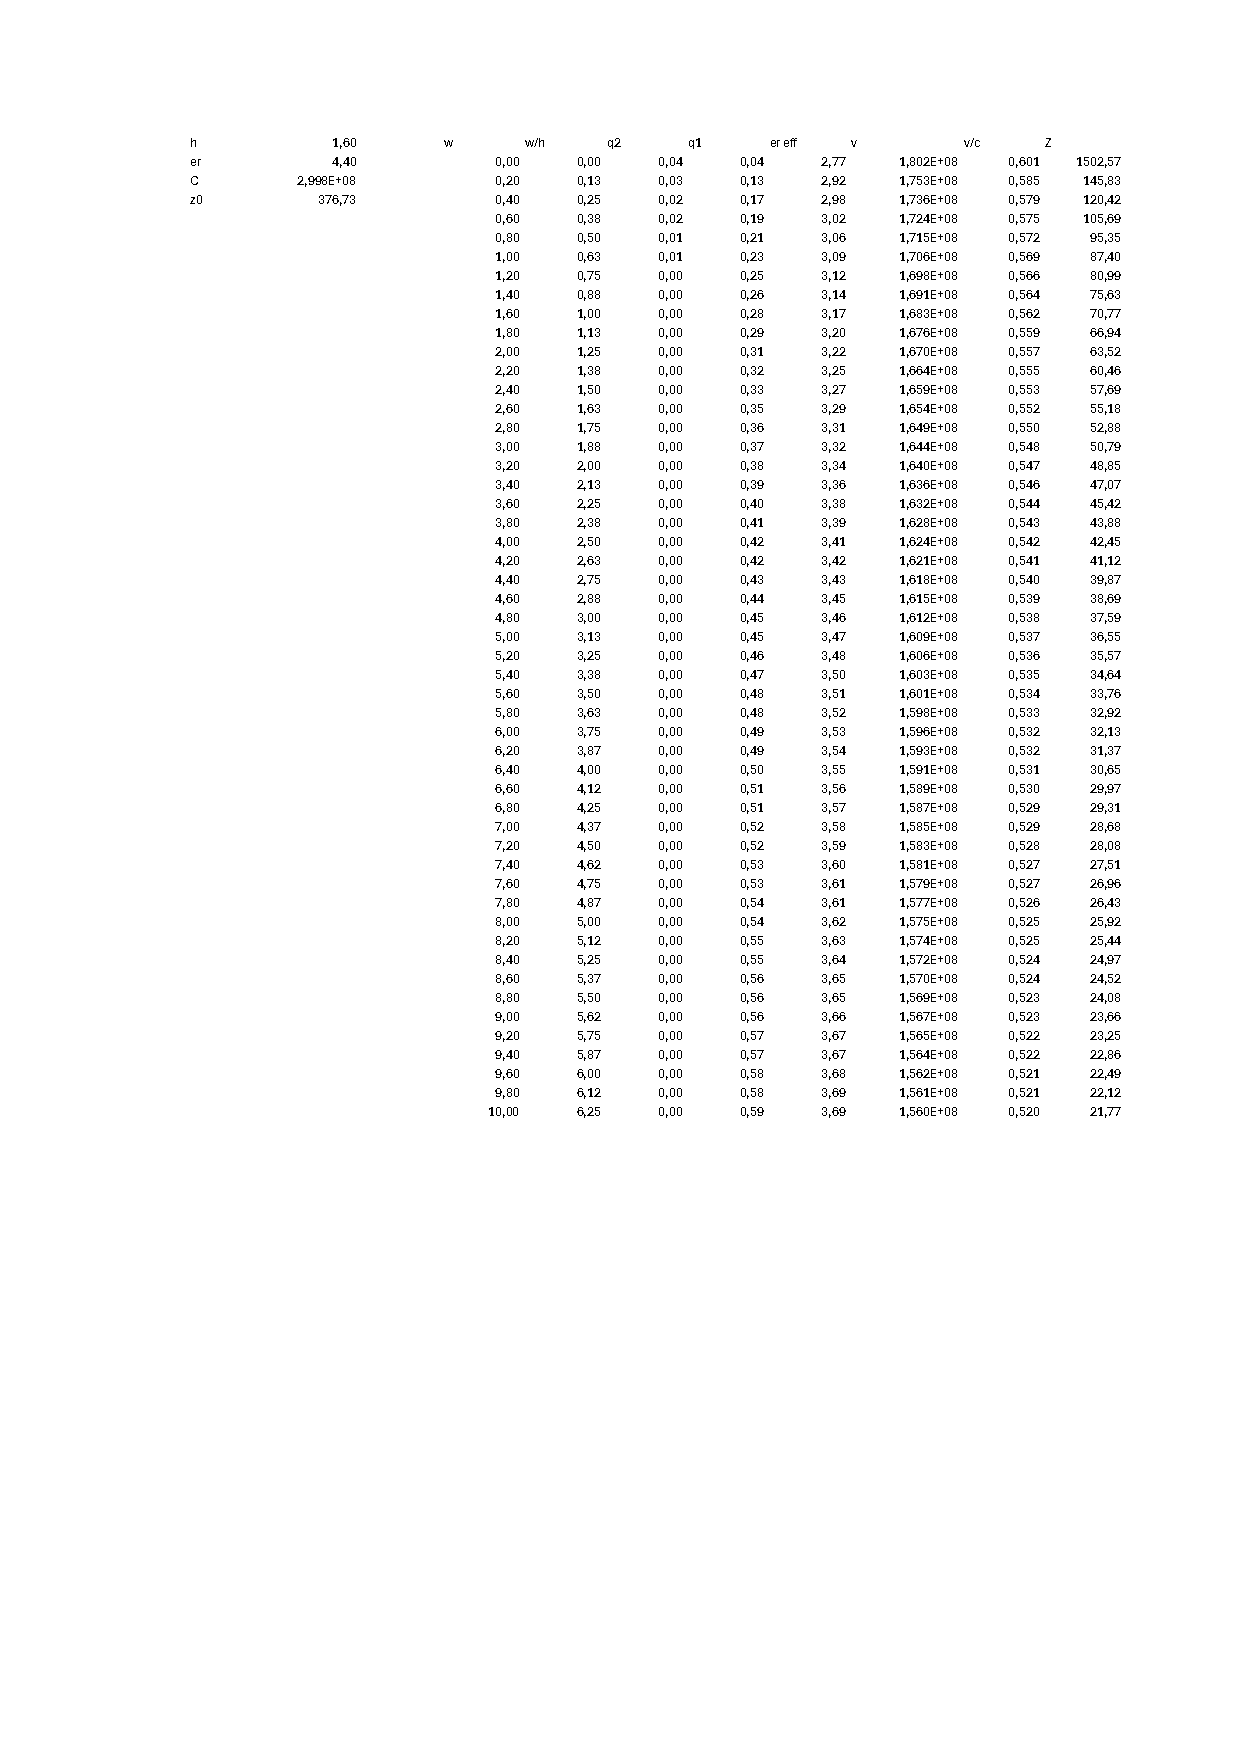
\includepdf{FeuilCalcMicrostrip.pdf}

\newpage
La \textbf{figure \ref{fig:microperm}} donne la permittivité effective d'une ligne microruban en fonction de la largeur de piste pour un substrat étant du FR4 de 1.6 mm d'épaisseur et avec $\epsilon_r=4.4$

\vspace{1cm}
\begin{figure}[h]
    \centering
    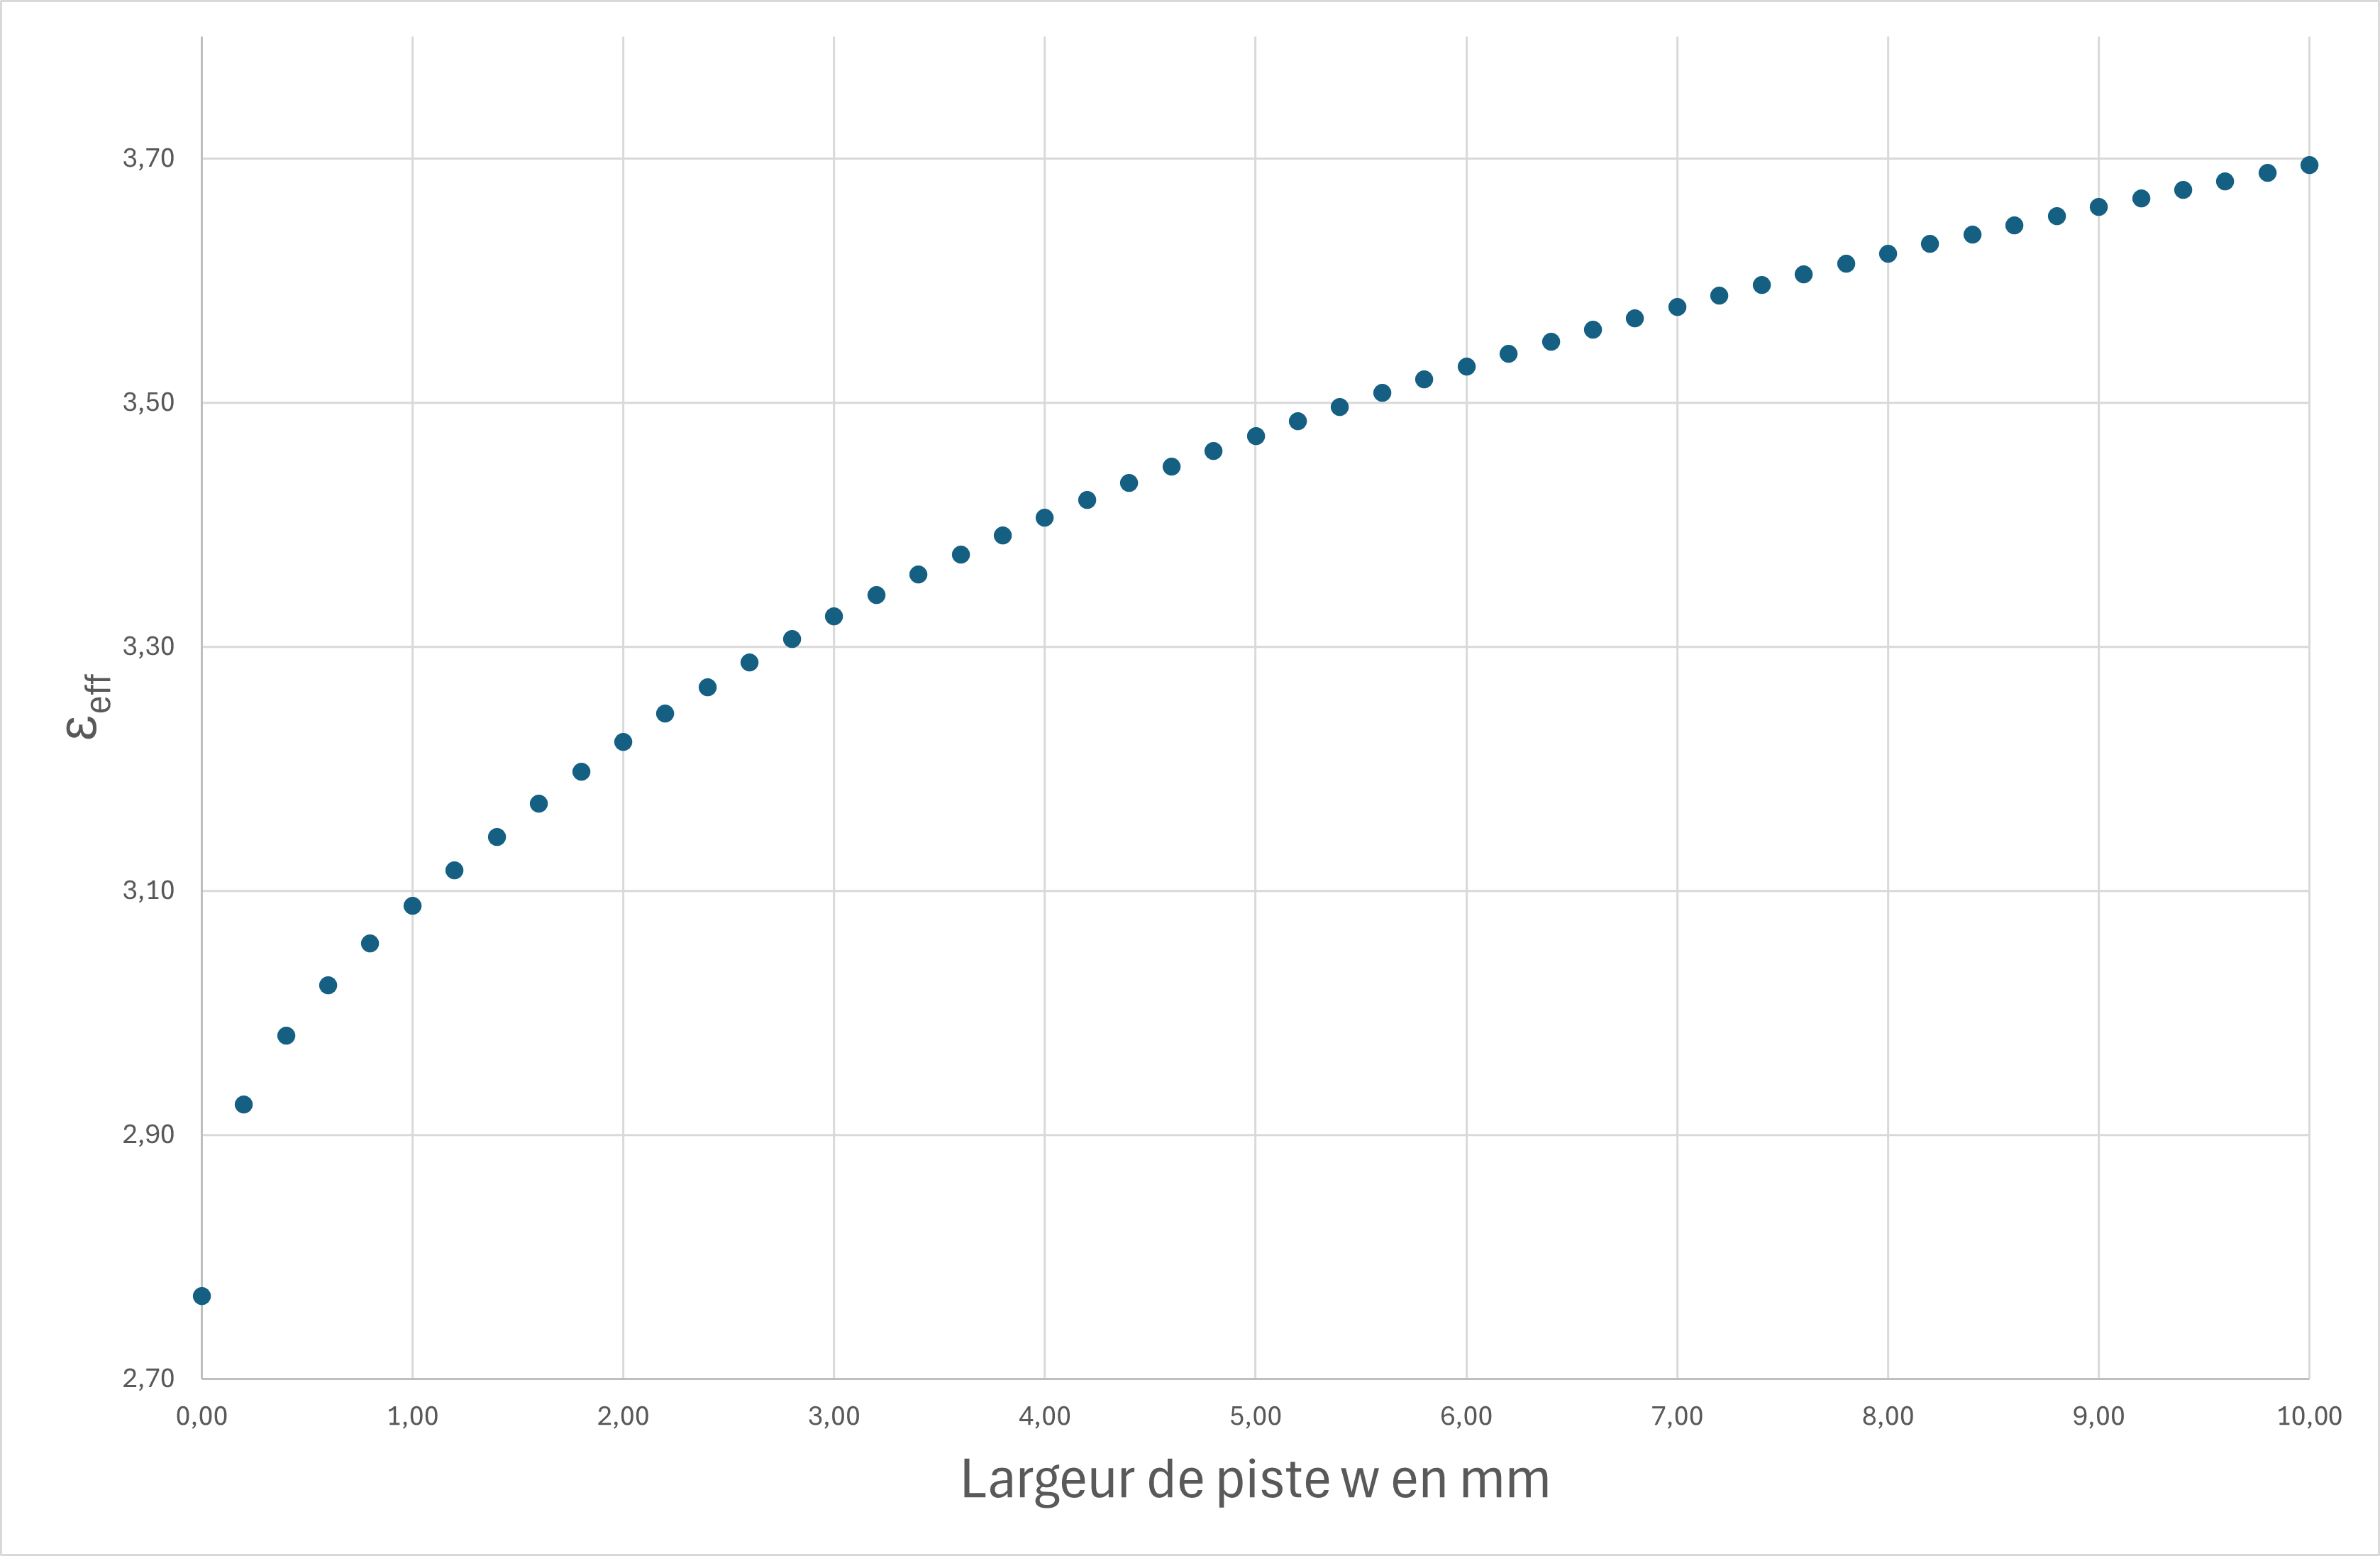
\includegraphics[scale=0.6]{images/microperm.png}
    \caption{Permittivité effective ligne microruban}
    \label{fig:microperm}
\end{figure}

\newpage
La \textbf{figure \ref{fig:microceler}} donne la célérité par rapport a la vitesse de la lumière dans le vide de l'onde dans une ligne microruban, en fonction de la largeur de piste avec les même paramètre que la \textbf{figure \ref{fig:microperm}}.

\vspace{1cm}
\begin{figure}[h]
    \centering
    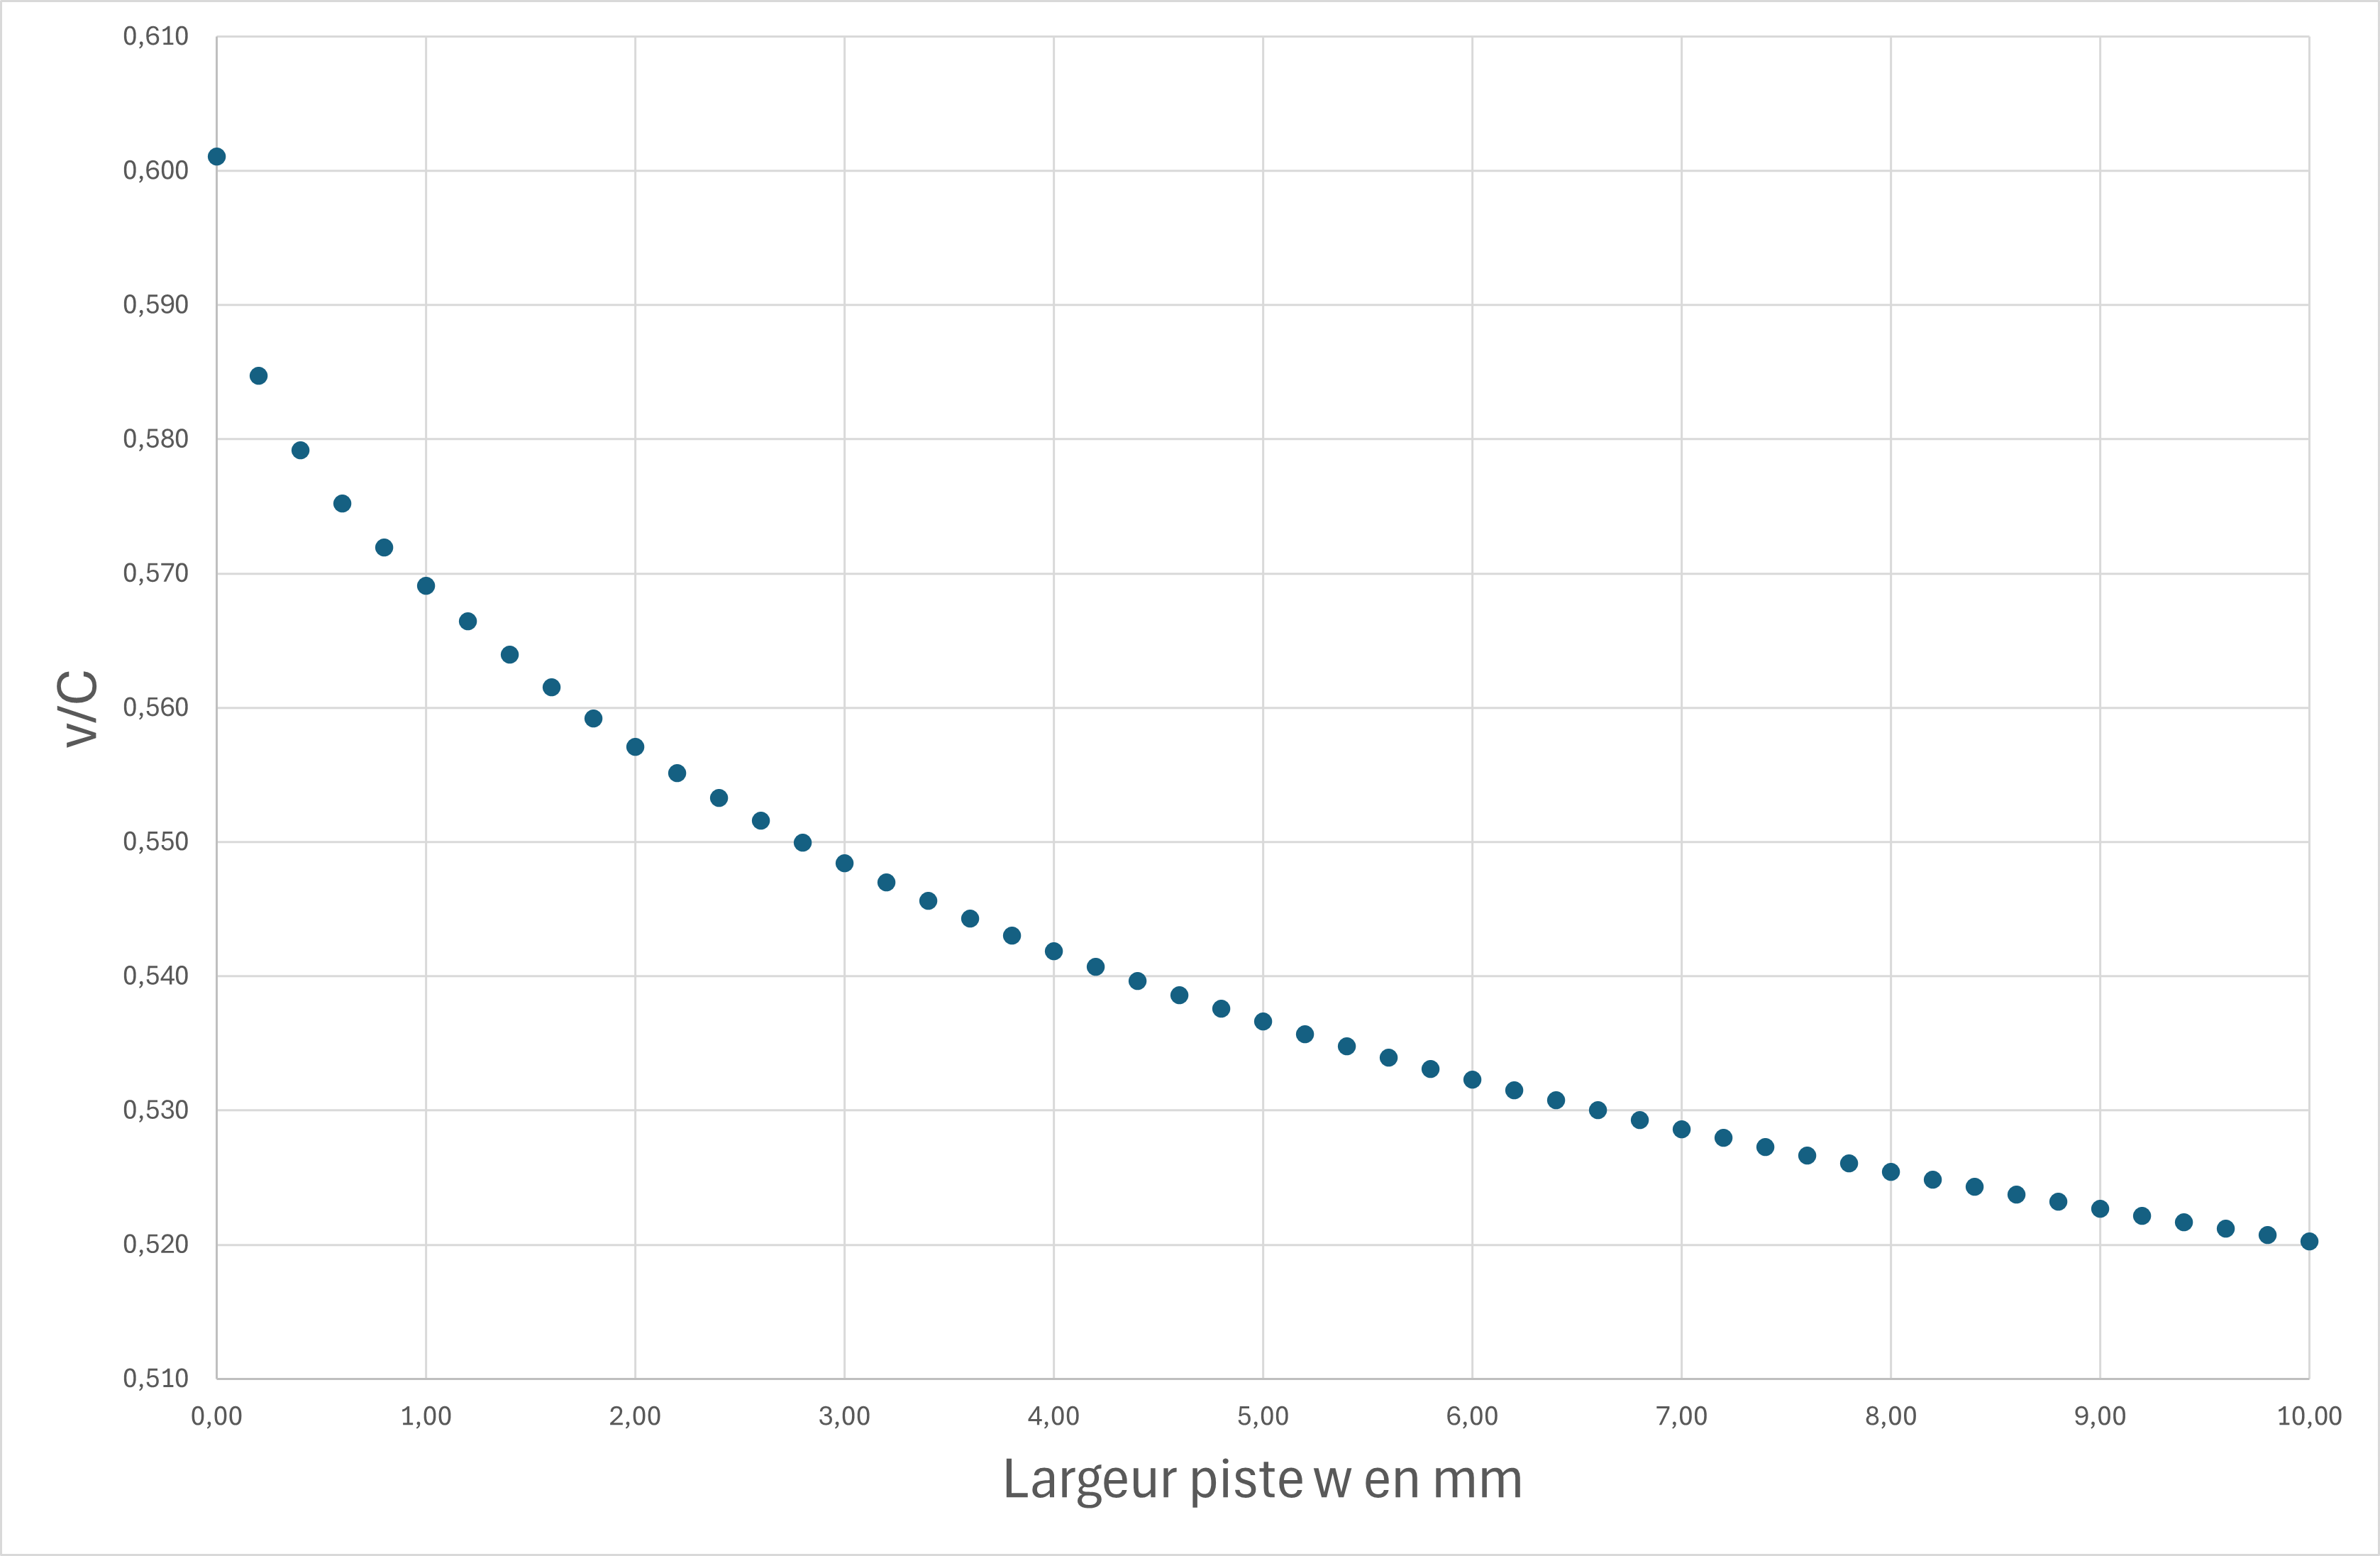
\includegraphics[scale=0.6]{images/microceler.png}
    \caption{Célérité ondes ligne microruban}
    \label{fig:microceler}
\end{figure}

\newpage
\normalsize{
\begin{equation}
\begin{aligned}
&v_1 = 0.61 \times C = 0.61 \times 3 \times 10^{8} = 1.83 \times 10^{8} \quad \text{m/s} \\
&v_2 = 0.52 \times C = 0.52 \times 3 \times 10^{8} = 1.56 \times 10^{8} \quad \text{m/s} \\
\\
&\text{Temps de propagation sur 1 mètre dans le guide 1 :} \\
&t_1 = \frac{1}{v_1} = \frac{1}{1.83 \times 10^{8}} \approx 5.4645 \times 10^{-9} \quad \text{s} \\
\\
&\text{Temps de propagation sur 1 mètre dans le guide 2 :} \\
&t_2 = \frac{1}{v_2} = \frac{1}{1.56 \times 10^{8}} \approx 6.4103 \times 10^{-9} \quad \text{s} \\
\\
&\text{Différence de temps entre les deux ondes :} \\
&\Delta t = t_2 - t_1 = 6.4103 \times 10^{-9} - 5.4645 \times 10^{-9} = 0.9458 \times 10^{-9} = 9.458 \times 10^{-10} \quad \text{s} \\
\\
&
\Delta t \approx 0.946 \, \text{nanosecondes (ns)}
\end{aligned}
\label{eq:timediffmicro}
\end{equation}
}
\vspace{1cm}

\newpage
La \textbf{figure \ref{fig:microimped}} donne l'impédance de la ligne par rapport à la largeur de piste avec les même paramètres que pour la permittivité effective et la célérité.

\vspace{1cm}
\begin{figure}[h]
    \centering
    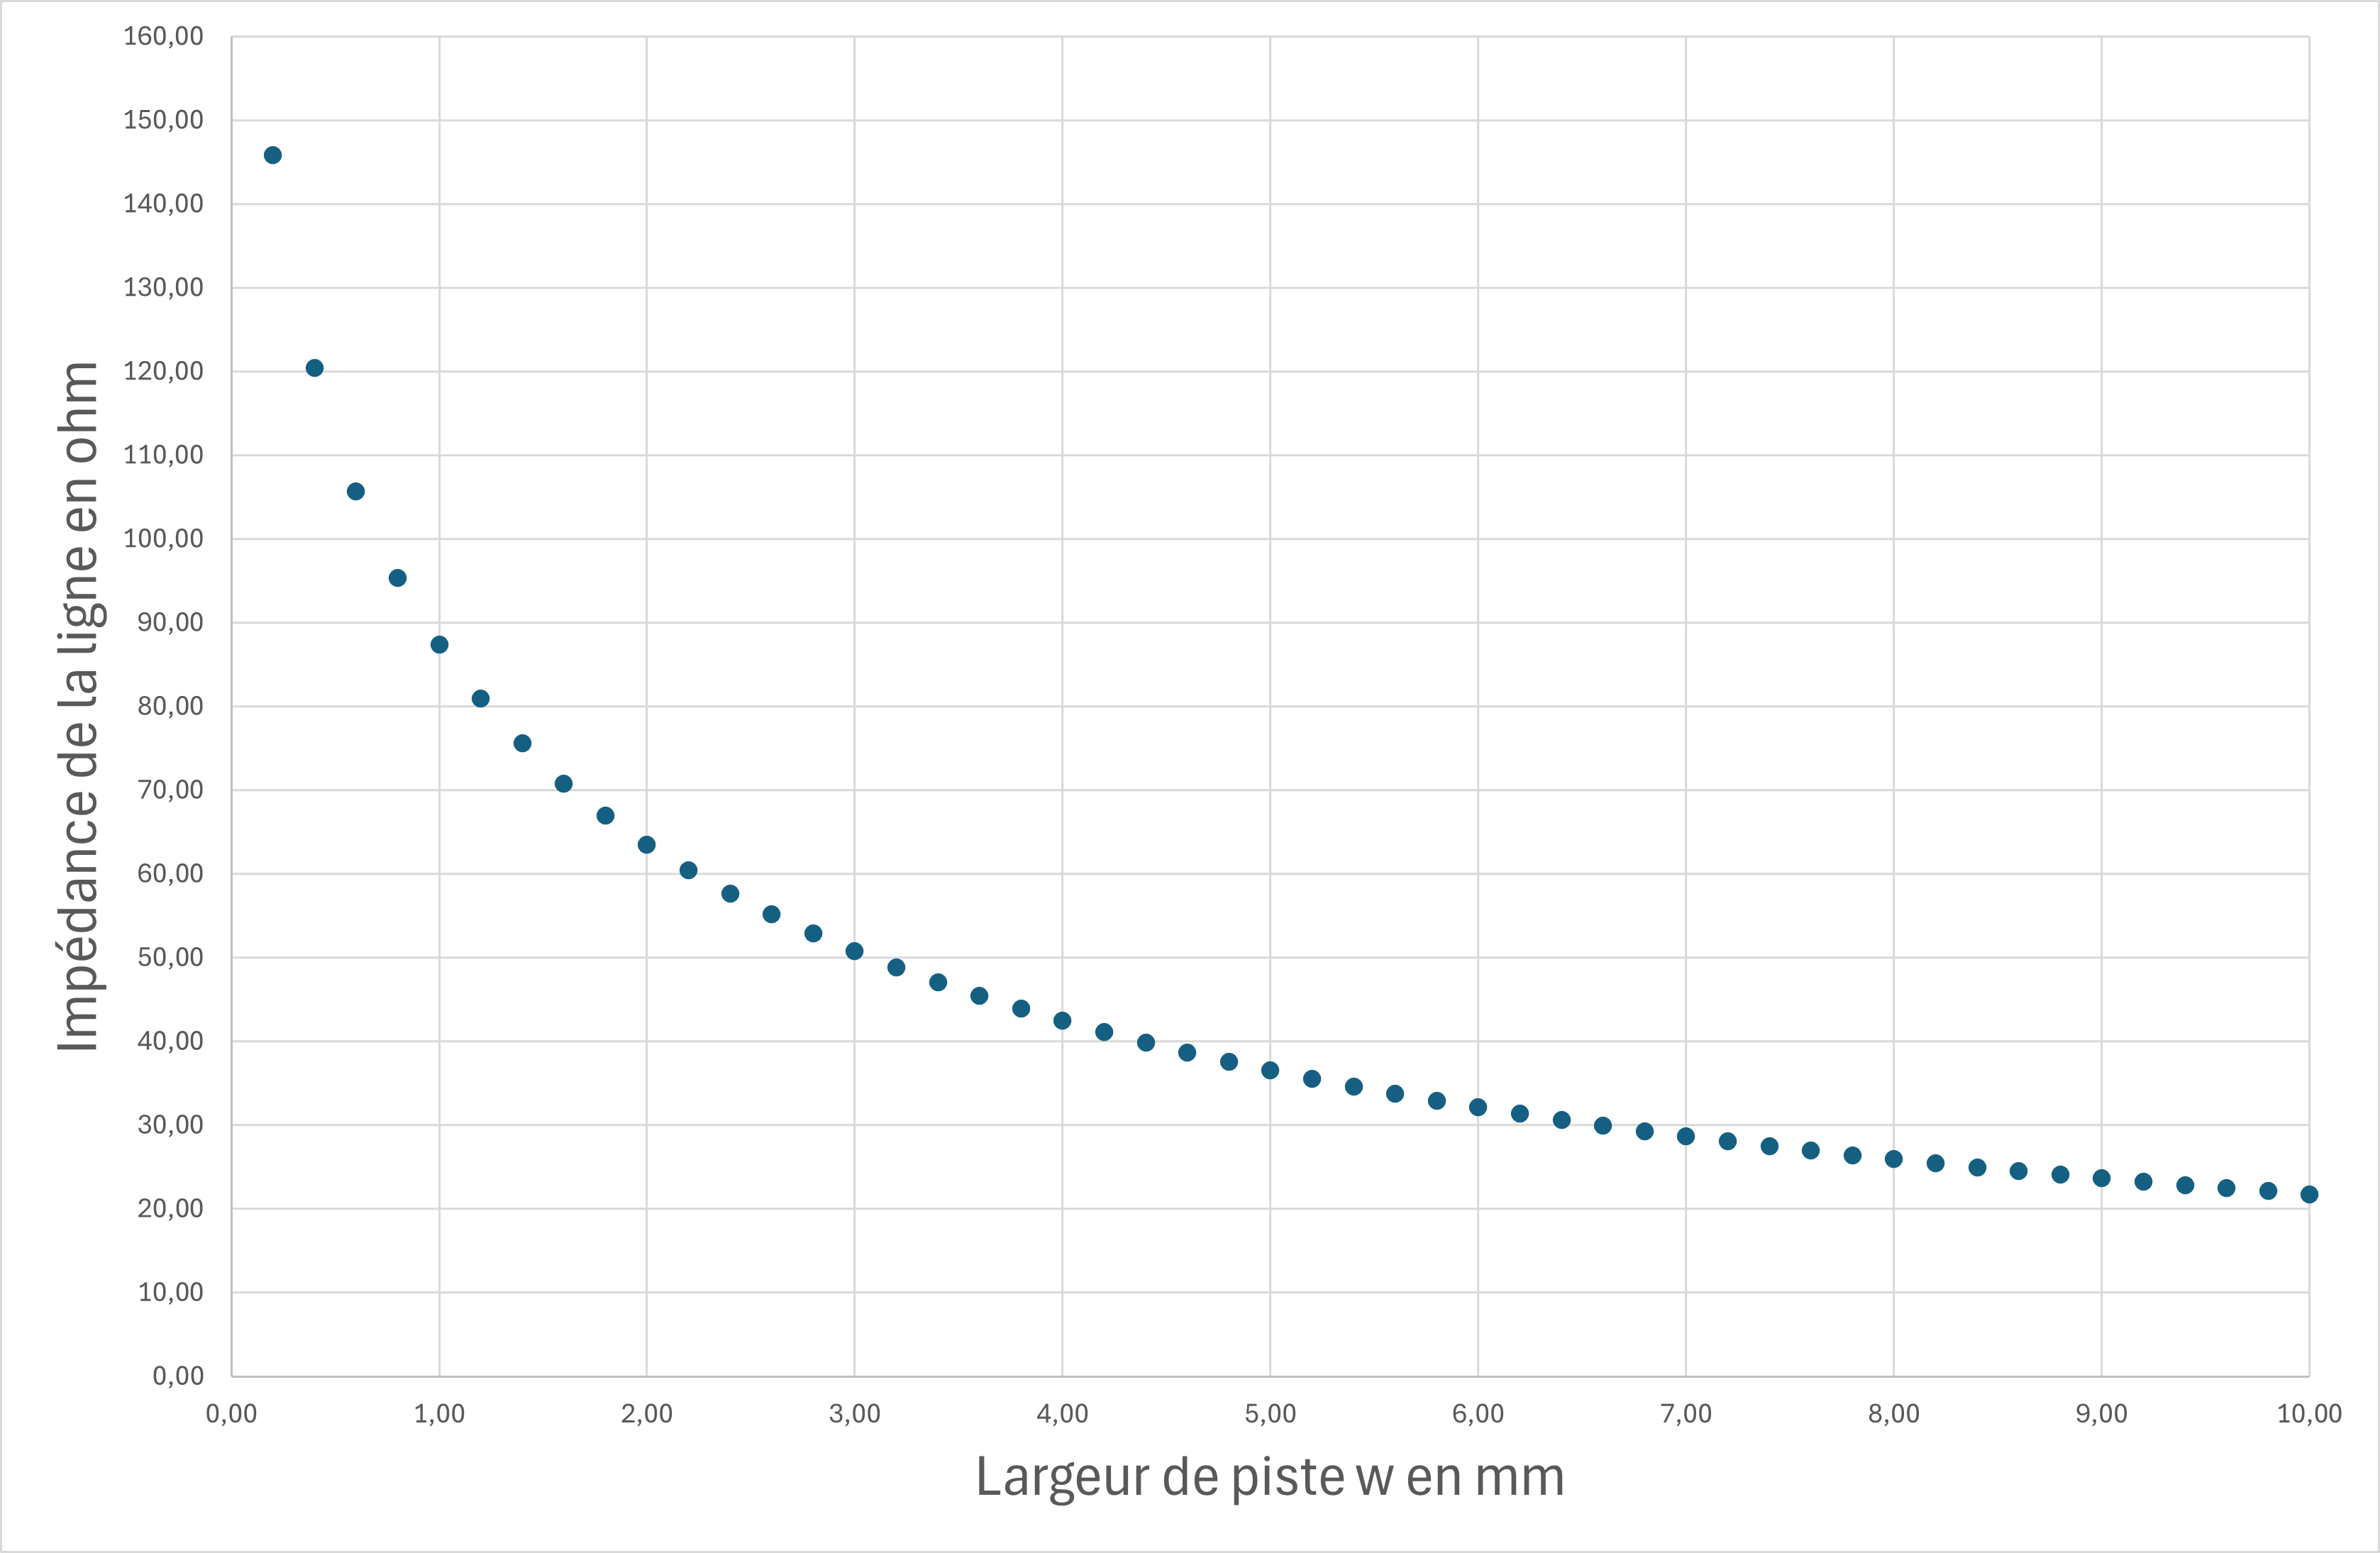
\includegraphics[scale=0.6]{images/microimped.png}
    \caption{Impedence ligne microruban}
    \label{fig:microimped}
\end{figure}

\newpage
La \textbf{figure \ref{fig:cpwperm}} donne la permittivité effective d'une ligne coplanaire en fonction de la largeur de piste et du gap pour un substrat étant du FR4 de 1.6 mm d'épaisseur et avec $\epsilon_r=4.4$

\vspace{1cm}
\begin{figure}[h]
    \centering
    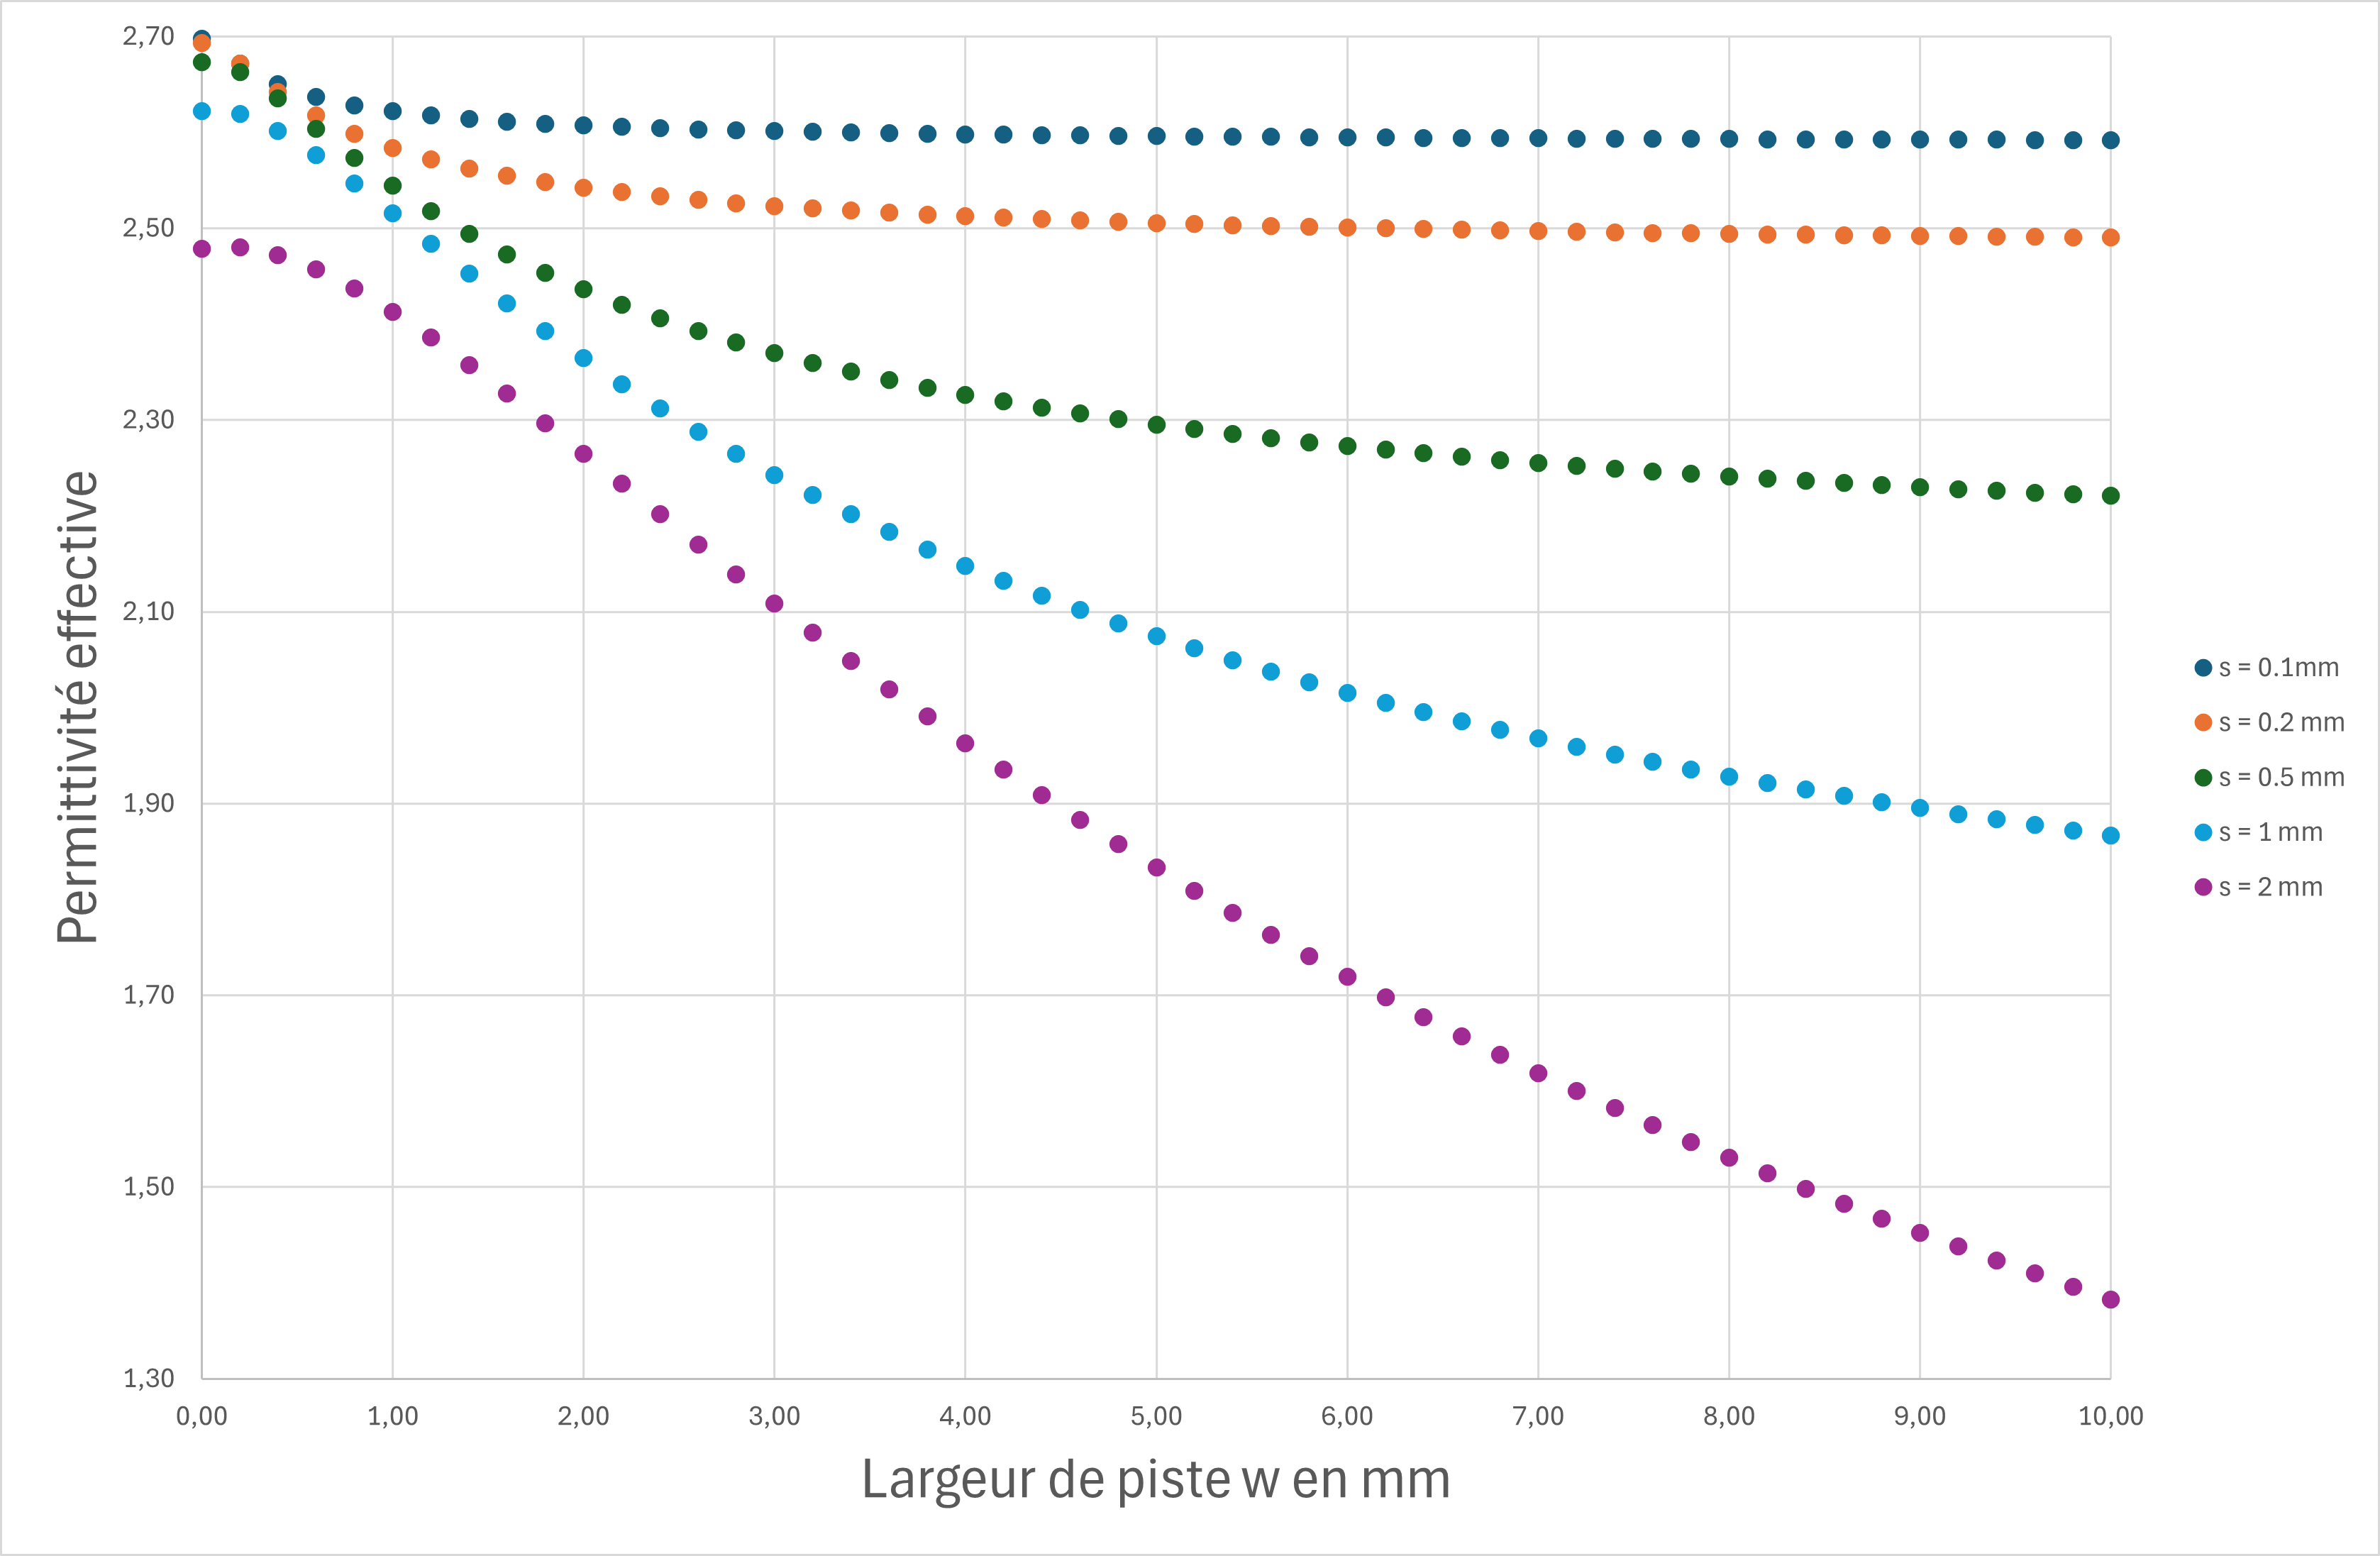
\includegraphics[scale=0.6]{images/cpwperm.png}
    \caption{Permittivité effective ligne coplanaire}
    \label{fig:cpwperm}
\end{figure}

\newpage
La \textbf{figure \ref{fig:cpwceler}} donne la célérité par rapport a la vitesse de la lumière dans le vide de l'onde dans une ligne coplanaire, en fonction de la largeur de piste et du gap avec les même paramètre que la \textbf{figure \ref{fig:cpwperm}}.

\vspace{1cm}
\begin{figure}[h]
    \centering
    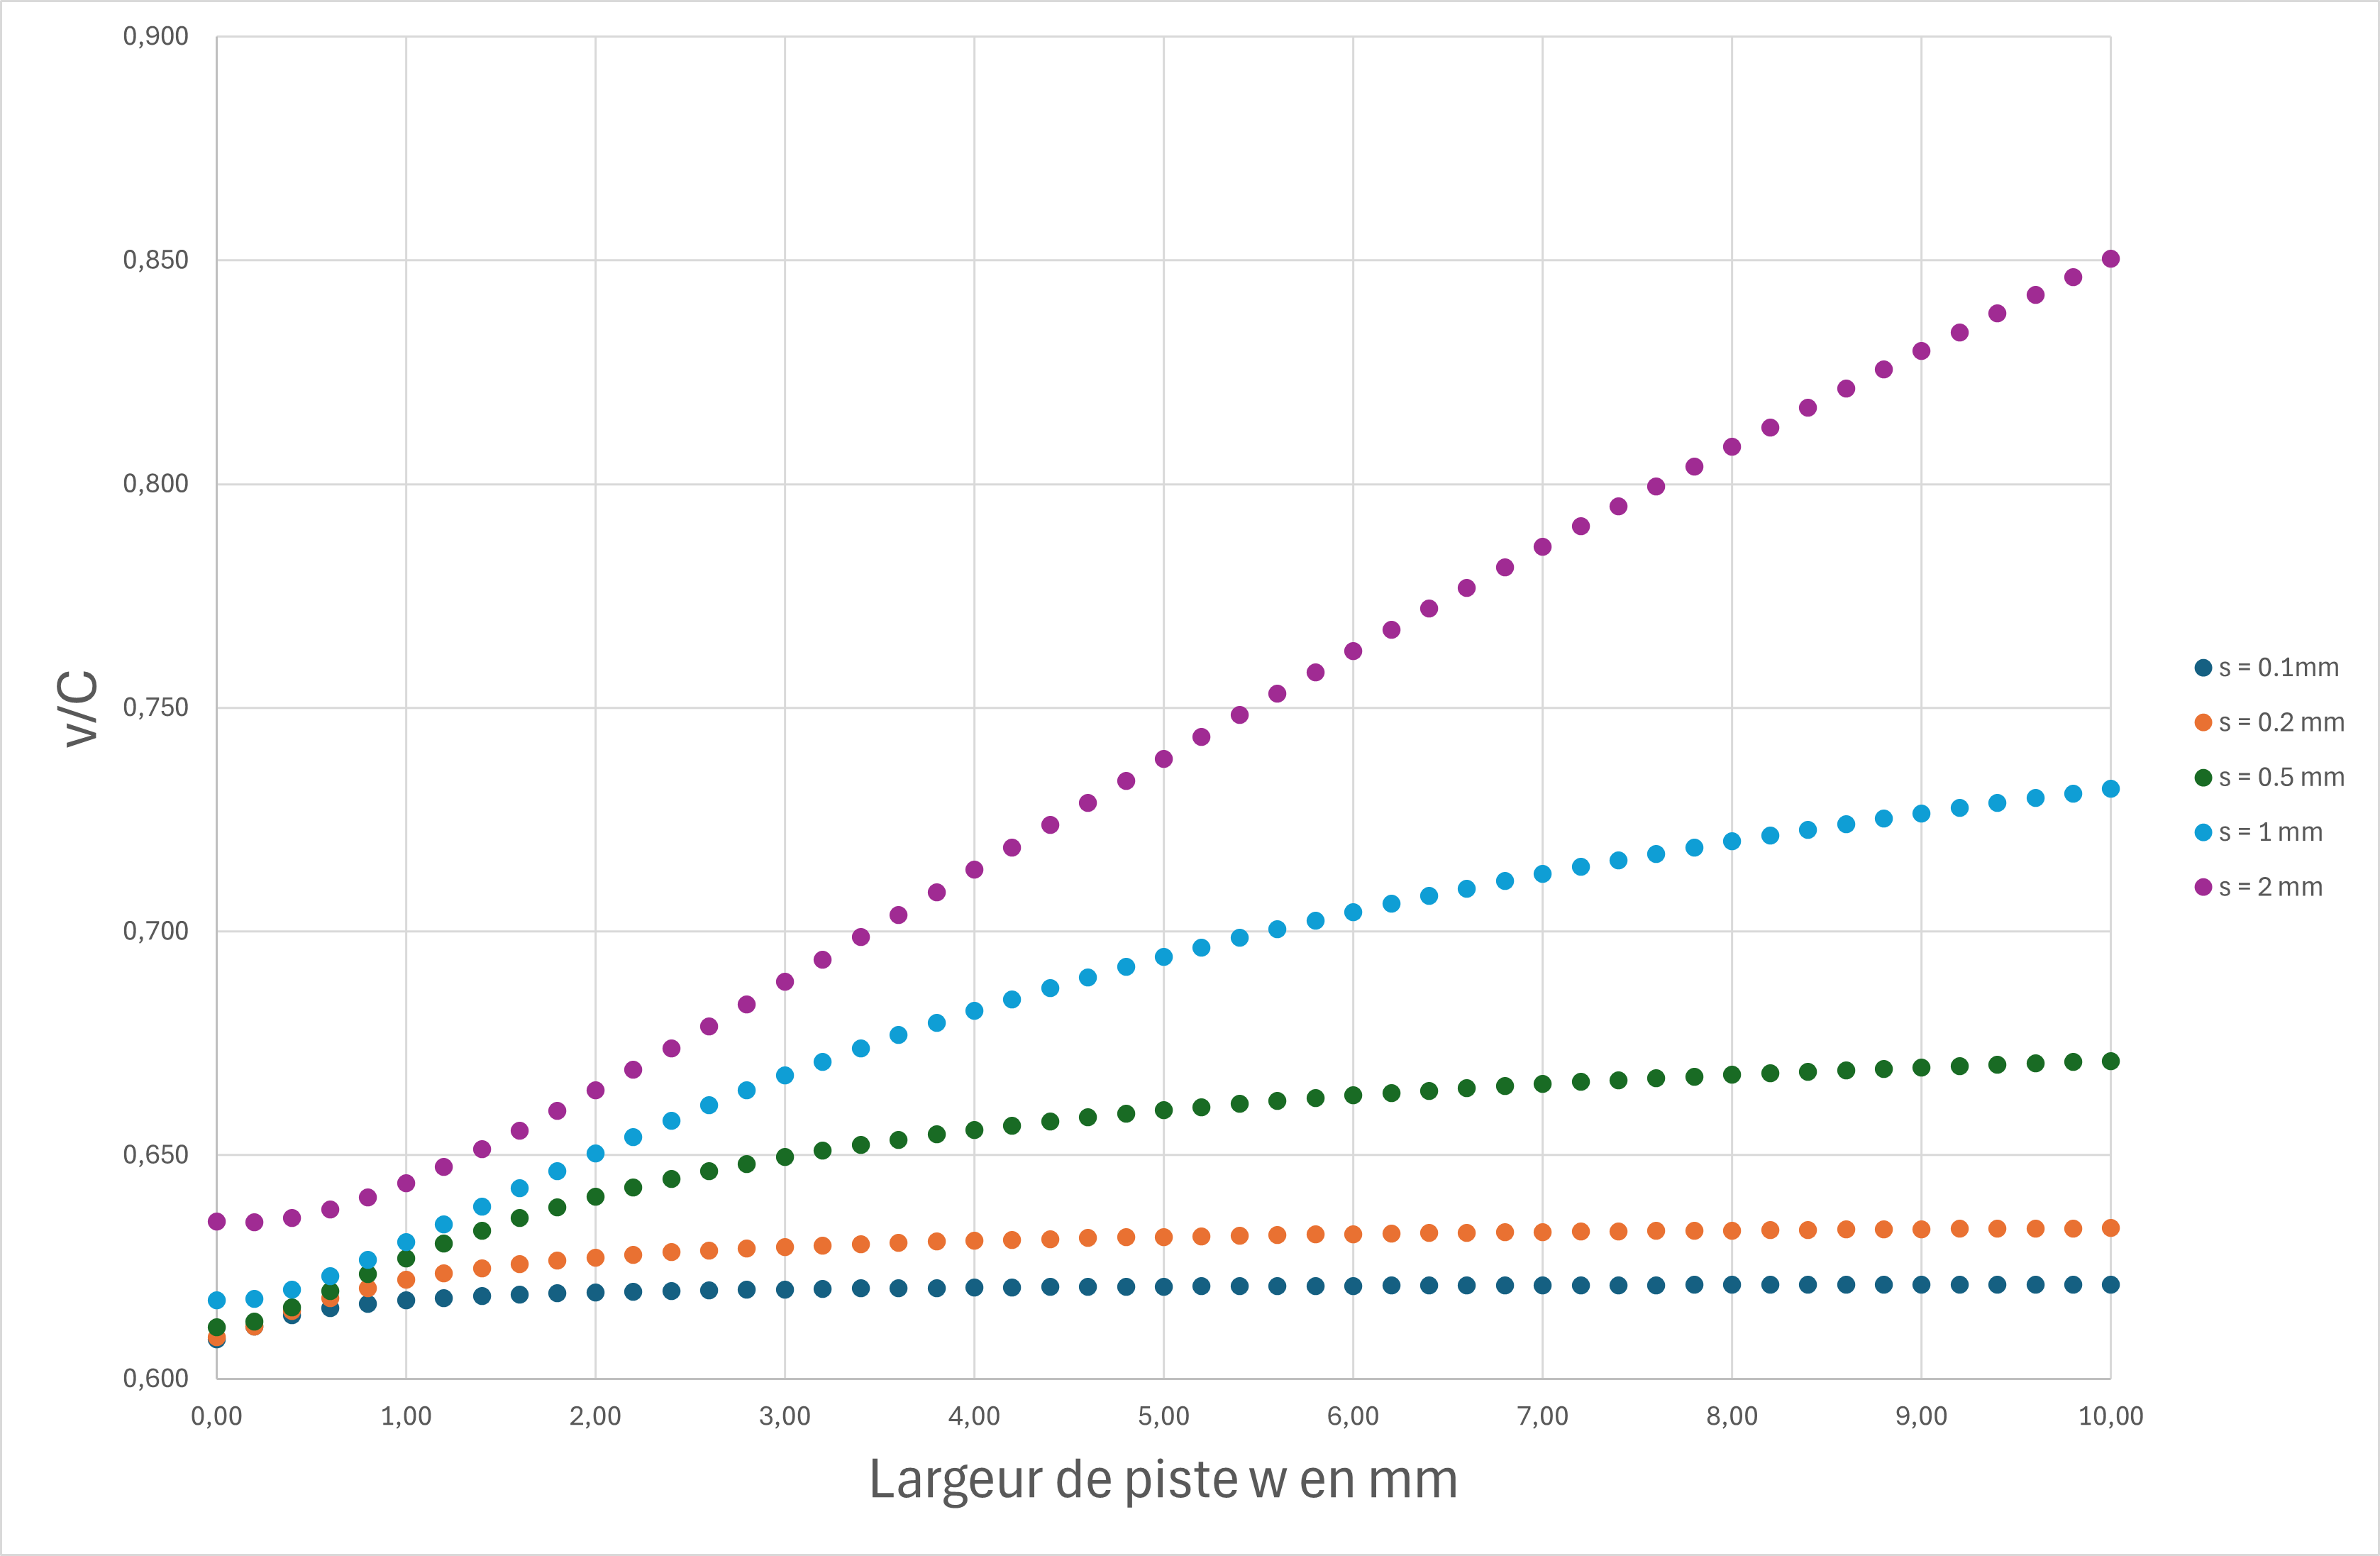
\includegraphics[scale=0.6]{images/cpwceler.png}
    \caption{Célérité ondes ligne coplanaire}
    \label{fig:cpwceler}
\end{figure}

\newpage
La \textbf{figure \ref{fig:cpwimped}} donne l'impédance d'une ligne coplanaire par rapport à la largeur de piste et du gap avec les même paramètres que pour la permittivité effective et la célérité.

\vspace{1cm}
\begin{figure}[h]
    \centering
    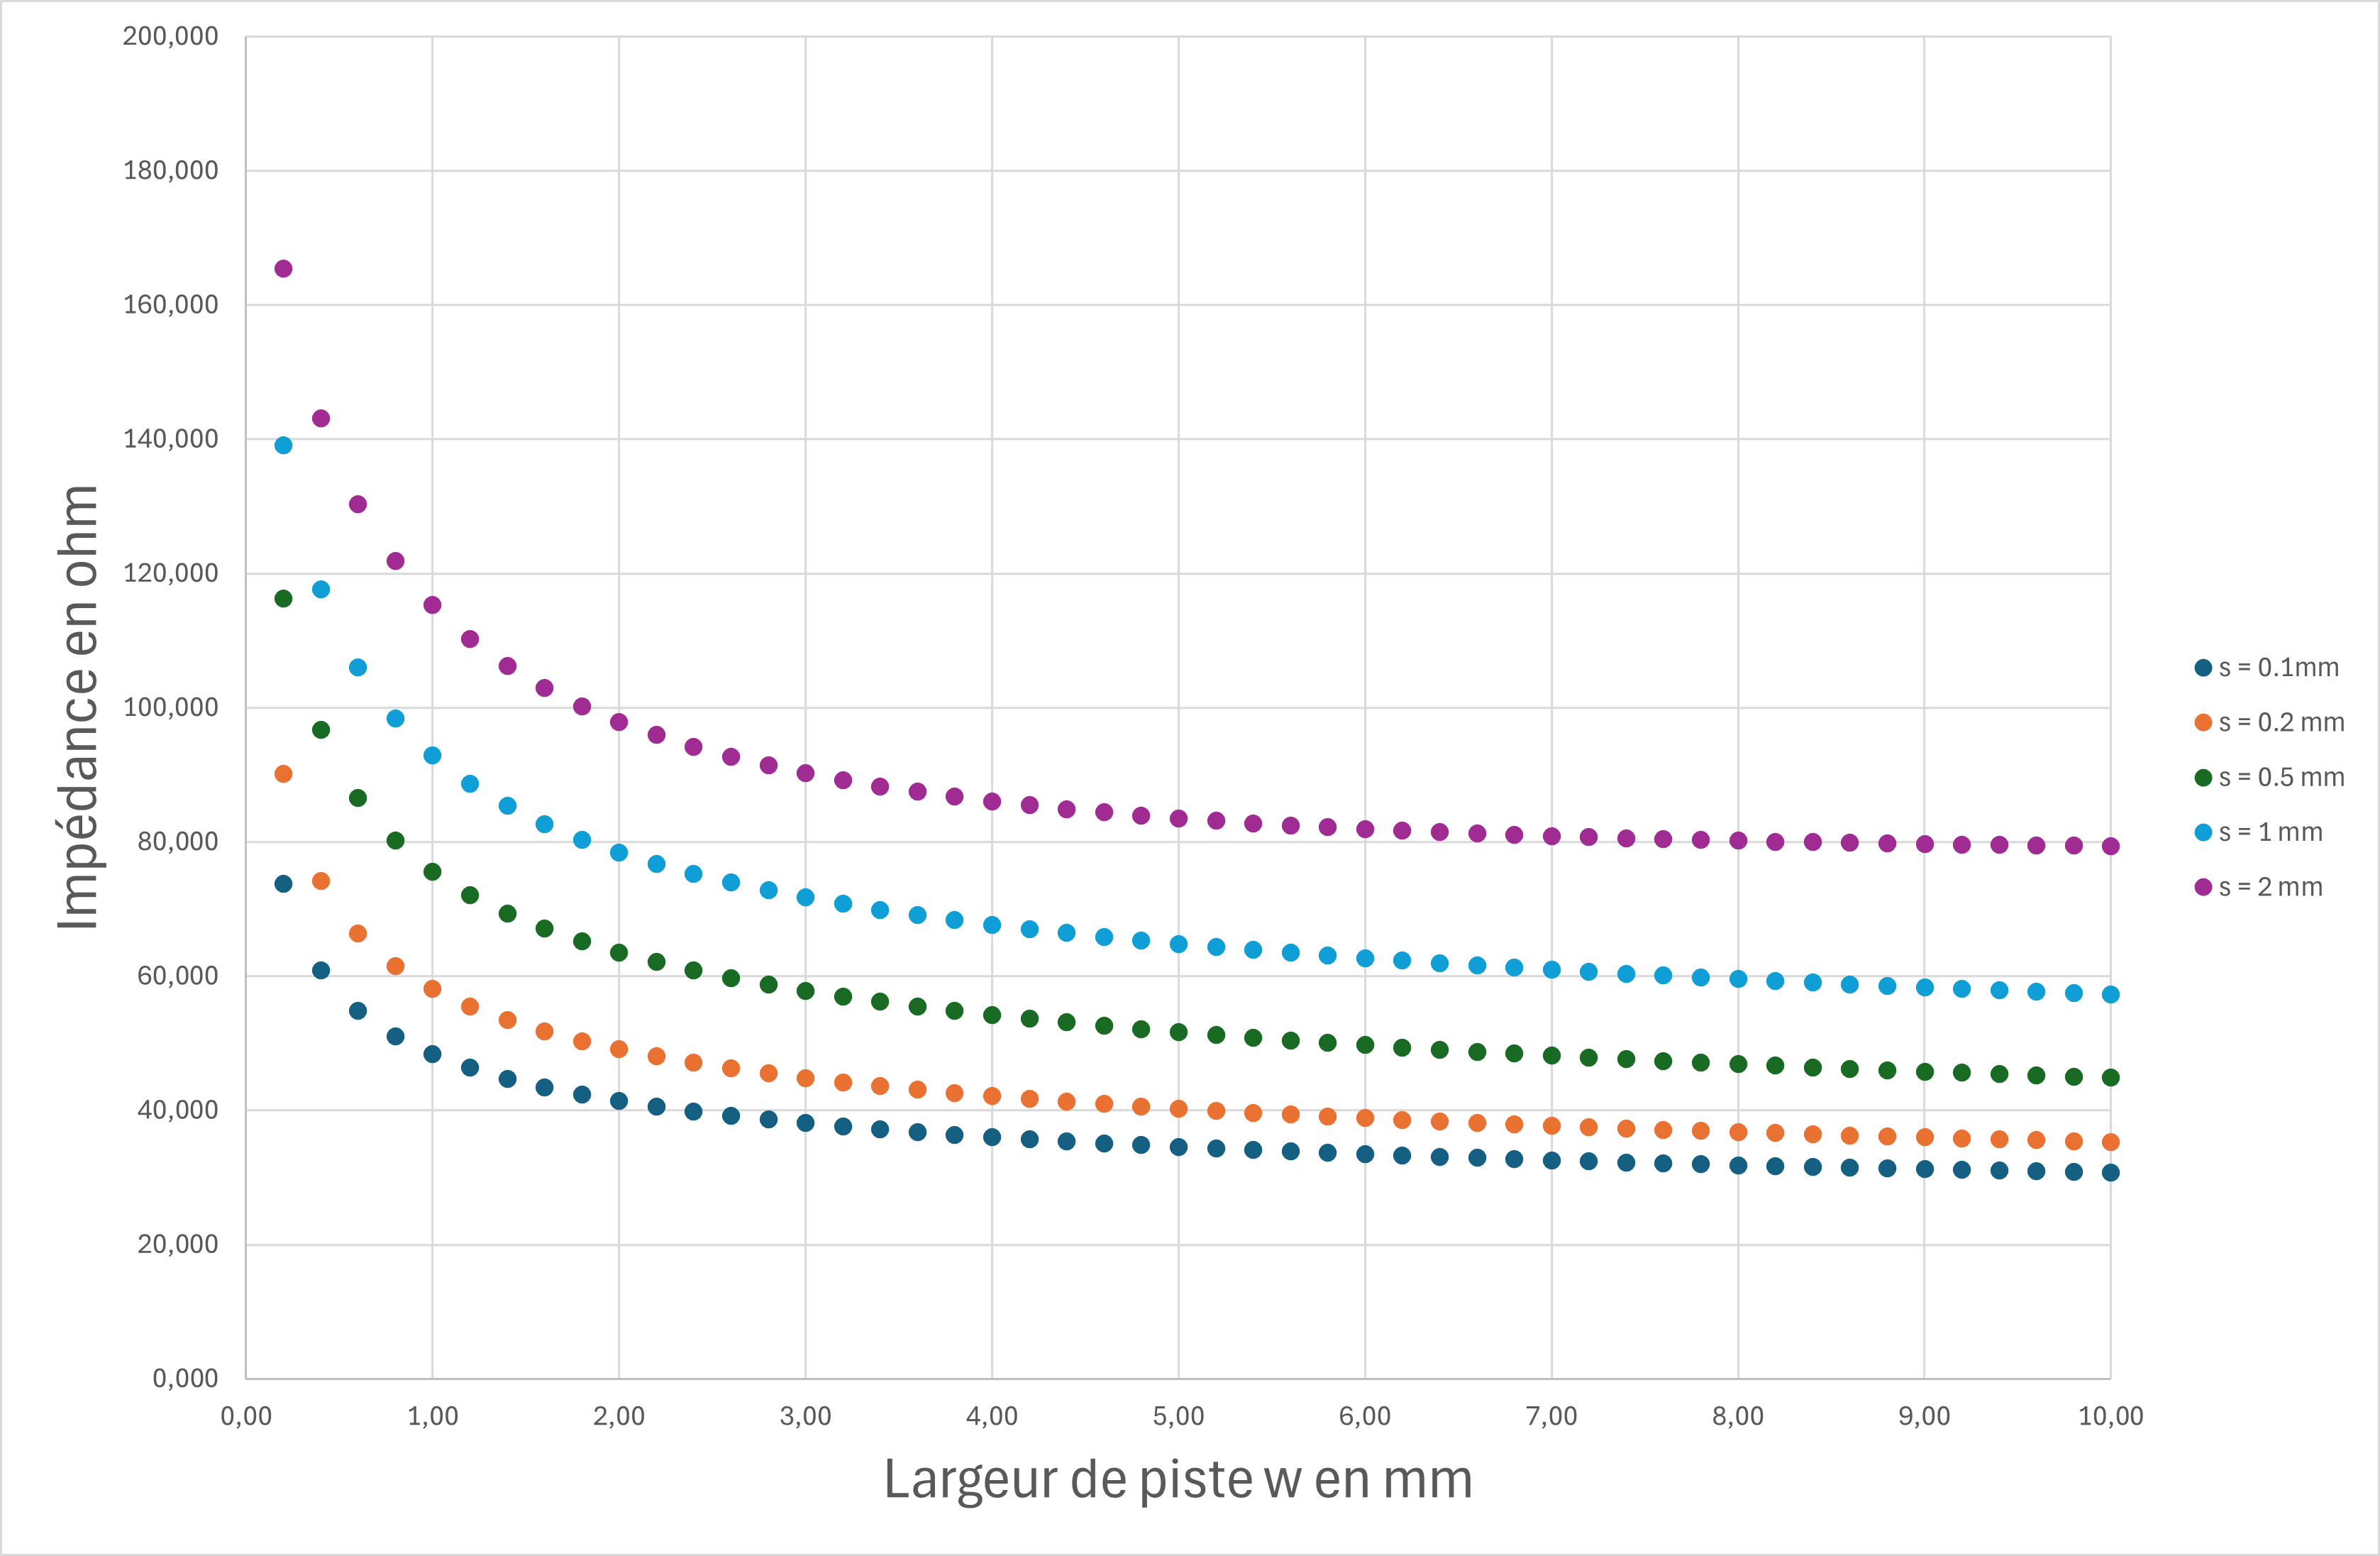
\includegraphics[scale=0.6]{images/cpwimped.png}
    \caption{Impédence ligne coplanaire}
    \label{fig:cpwimped}
\end{figure}

\newpage
\begin{figure}[h]
    \centering
    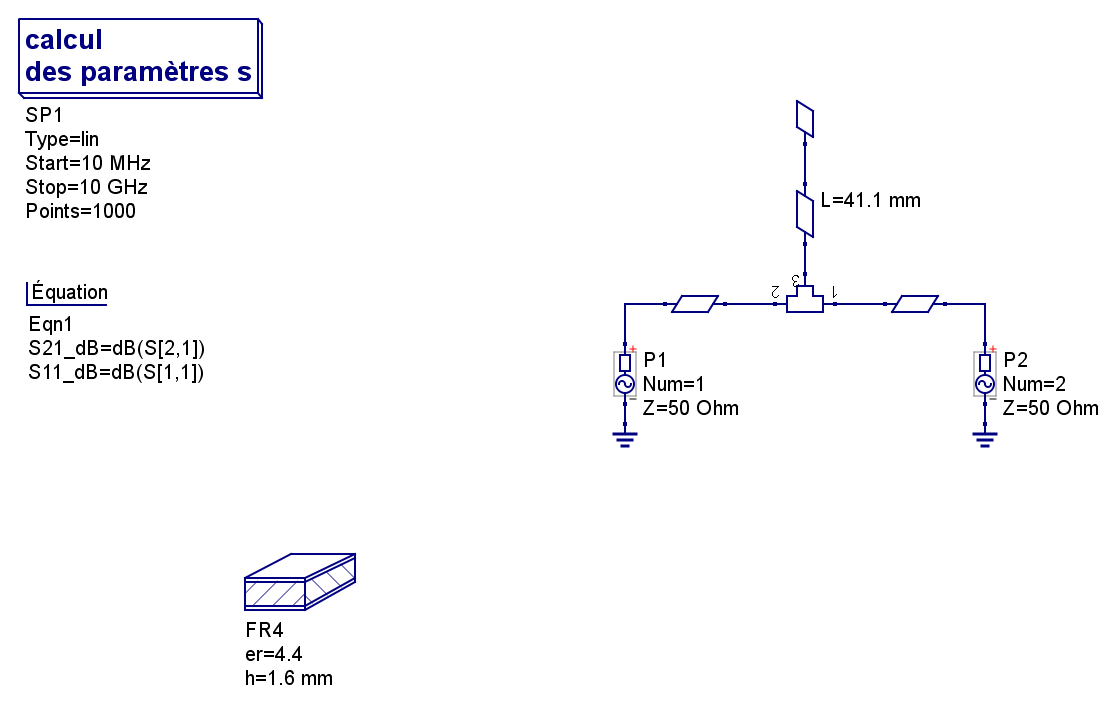
\includegraphics[scale=0.5]{images/openstubschema.png}
    \caption{Schéma Qucs stub ouvert}
    \label{fig:openstubschema}
\end{figure}

\vspace{1cm}
\begin{figure}[h]
    \centering
    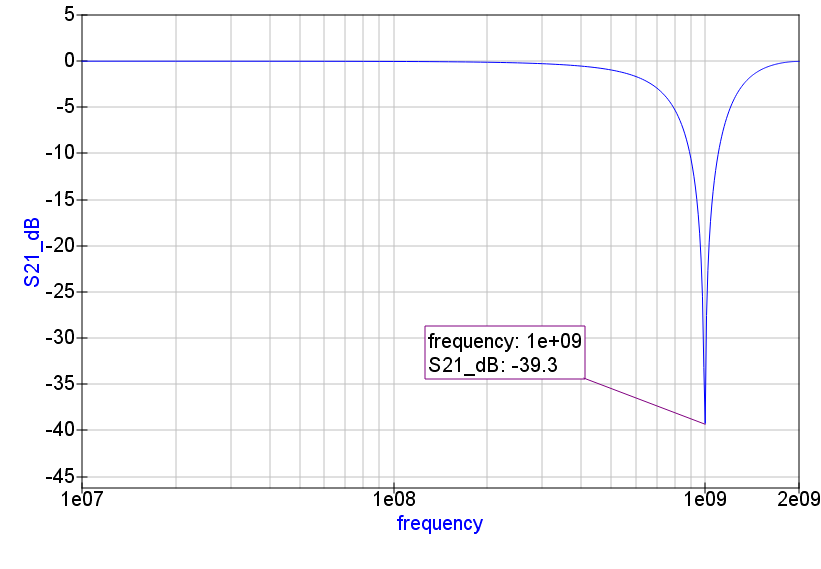
\includegraphics[scale=0.7]{images/openstubmeas.png}
    \caption{Résultat Qucs stub ouvert}
    \label{fig:openstubmeas2}
\end{figure}

\newpage
\vspace{1cm}
\begin{figure}[h]
    \centering
    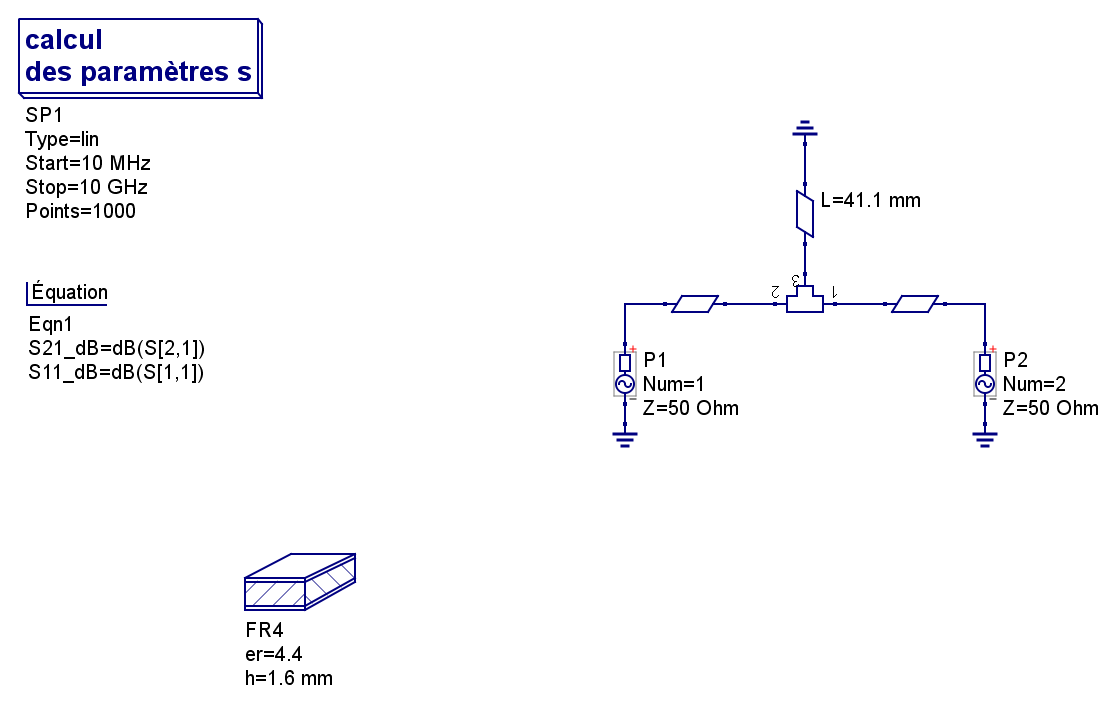
\includegraphics[scale=0.5]{images/shortstubschema.png}
    \caption{Schéma Qucs stub en cc}
    \label{fig:shortstubschema}
\end{figure}

\vspace{1cm}
\begin{figure}[h]
    \centering
    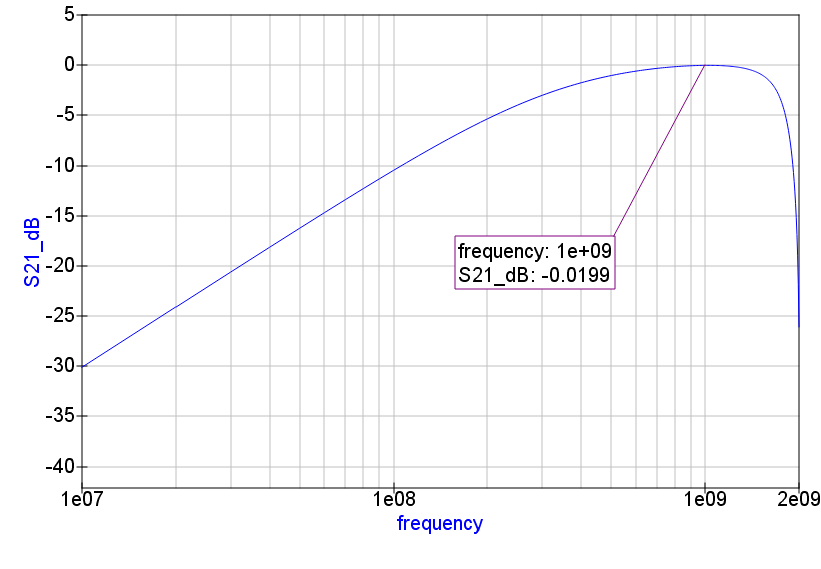
\includegraphics[scale=0.7]{images/shortstubmeas.png}
    \caption{Résultat Qucs stub en cc}
    \label{fig:shortstubmeas2}
\end{figure}

\newpage
\vspace{1cm}
\begin{figure}[h]
    \centering
    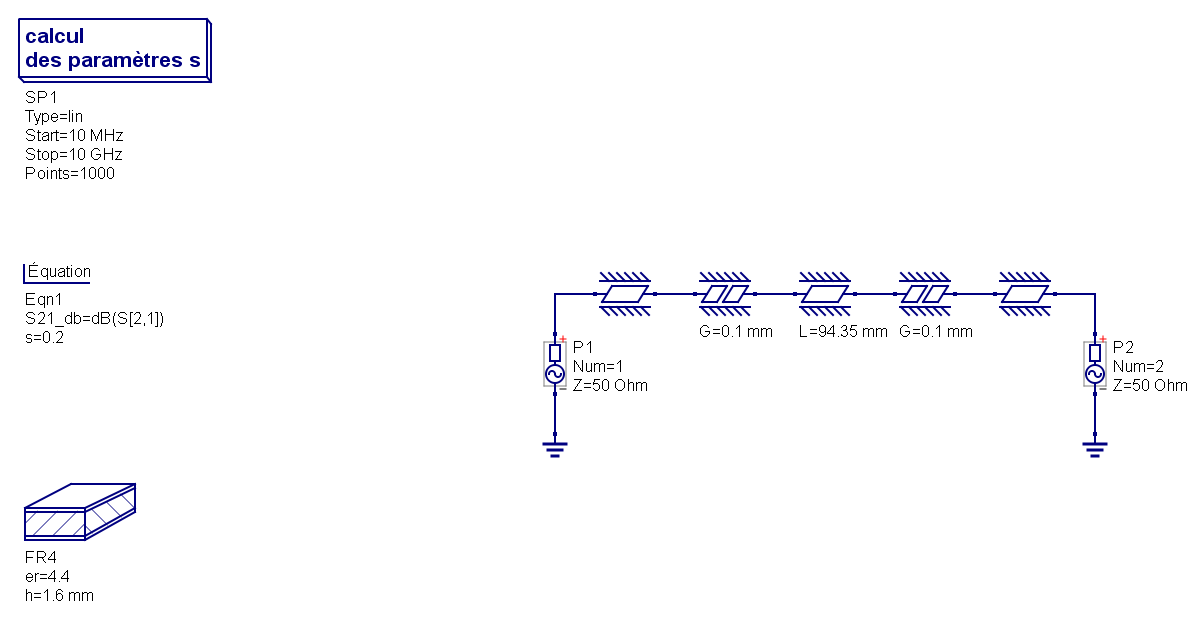
\includegraphics[scale=0.4]{images/halfqucsschema.png}
    \caption{Schéma Qucs résonateur demi onde}
    \label{fig:halfqucsschema}
\end{figure}

\vspace{1cm}
\begin{figure}[h]
    \centering
    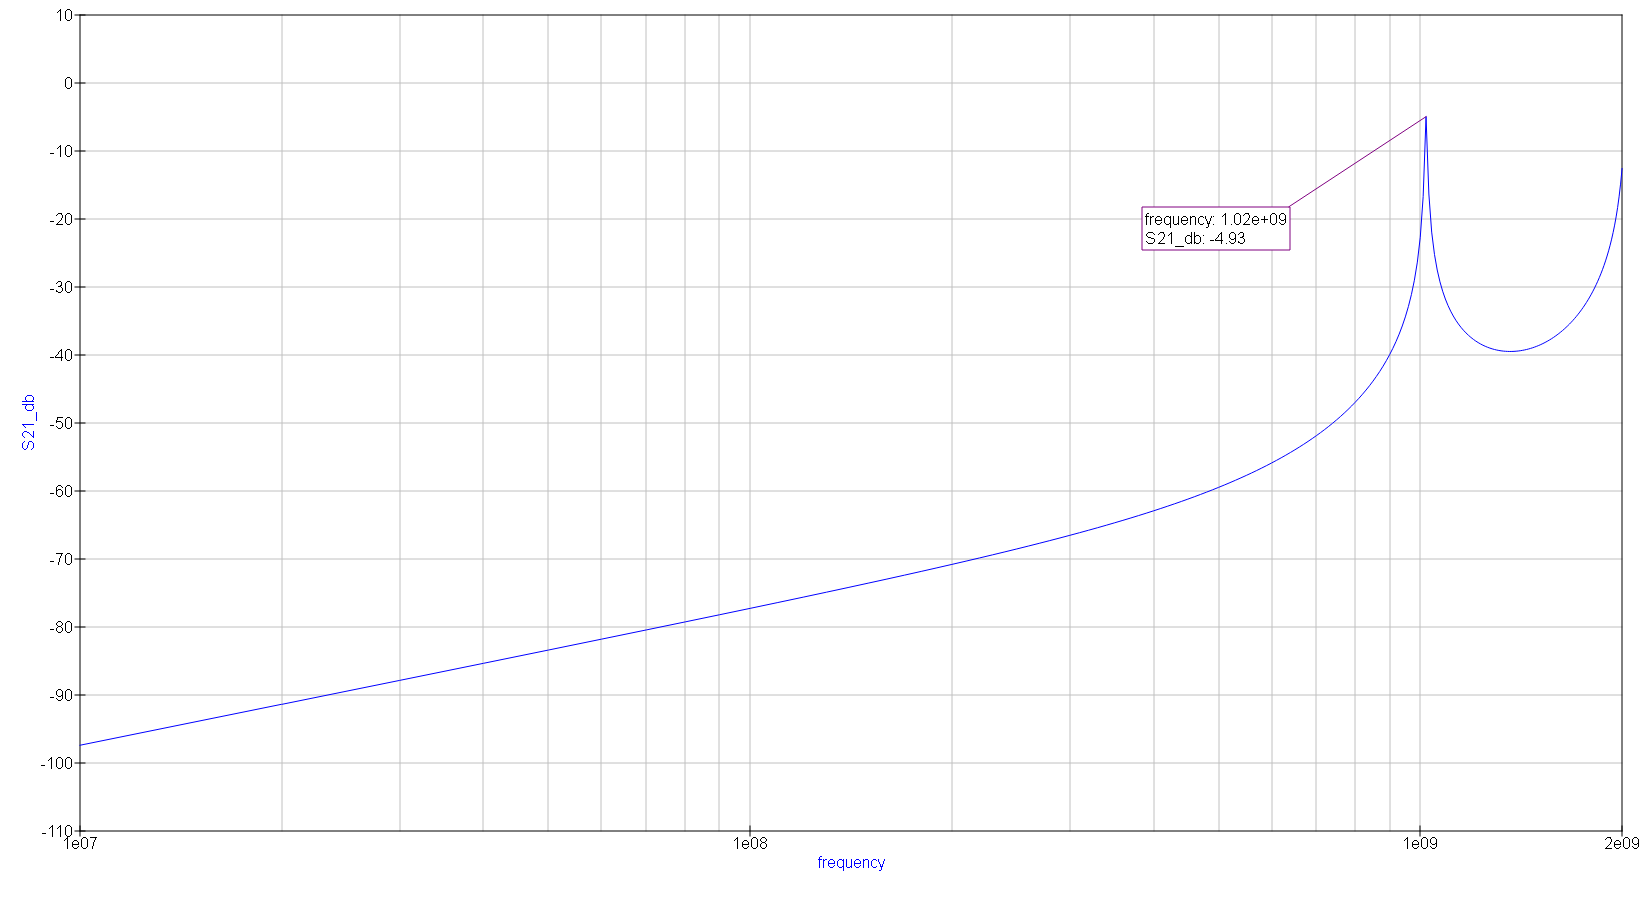
\includegraphics[scale=0.35]{images/halfqucsmeas.png}
    \caption{Résultat Qucs résonateur demi onde}
    \label{fig:halfqucsmeas2}
\end{figure}

\newpage
\subsection{Électronique}

La \textbf{figure \ref{fig:rf_emit_sch}} est le schéma électrique du module mikroBus d'emission.
\begin{figure}[h]
    \centering
    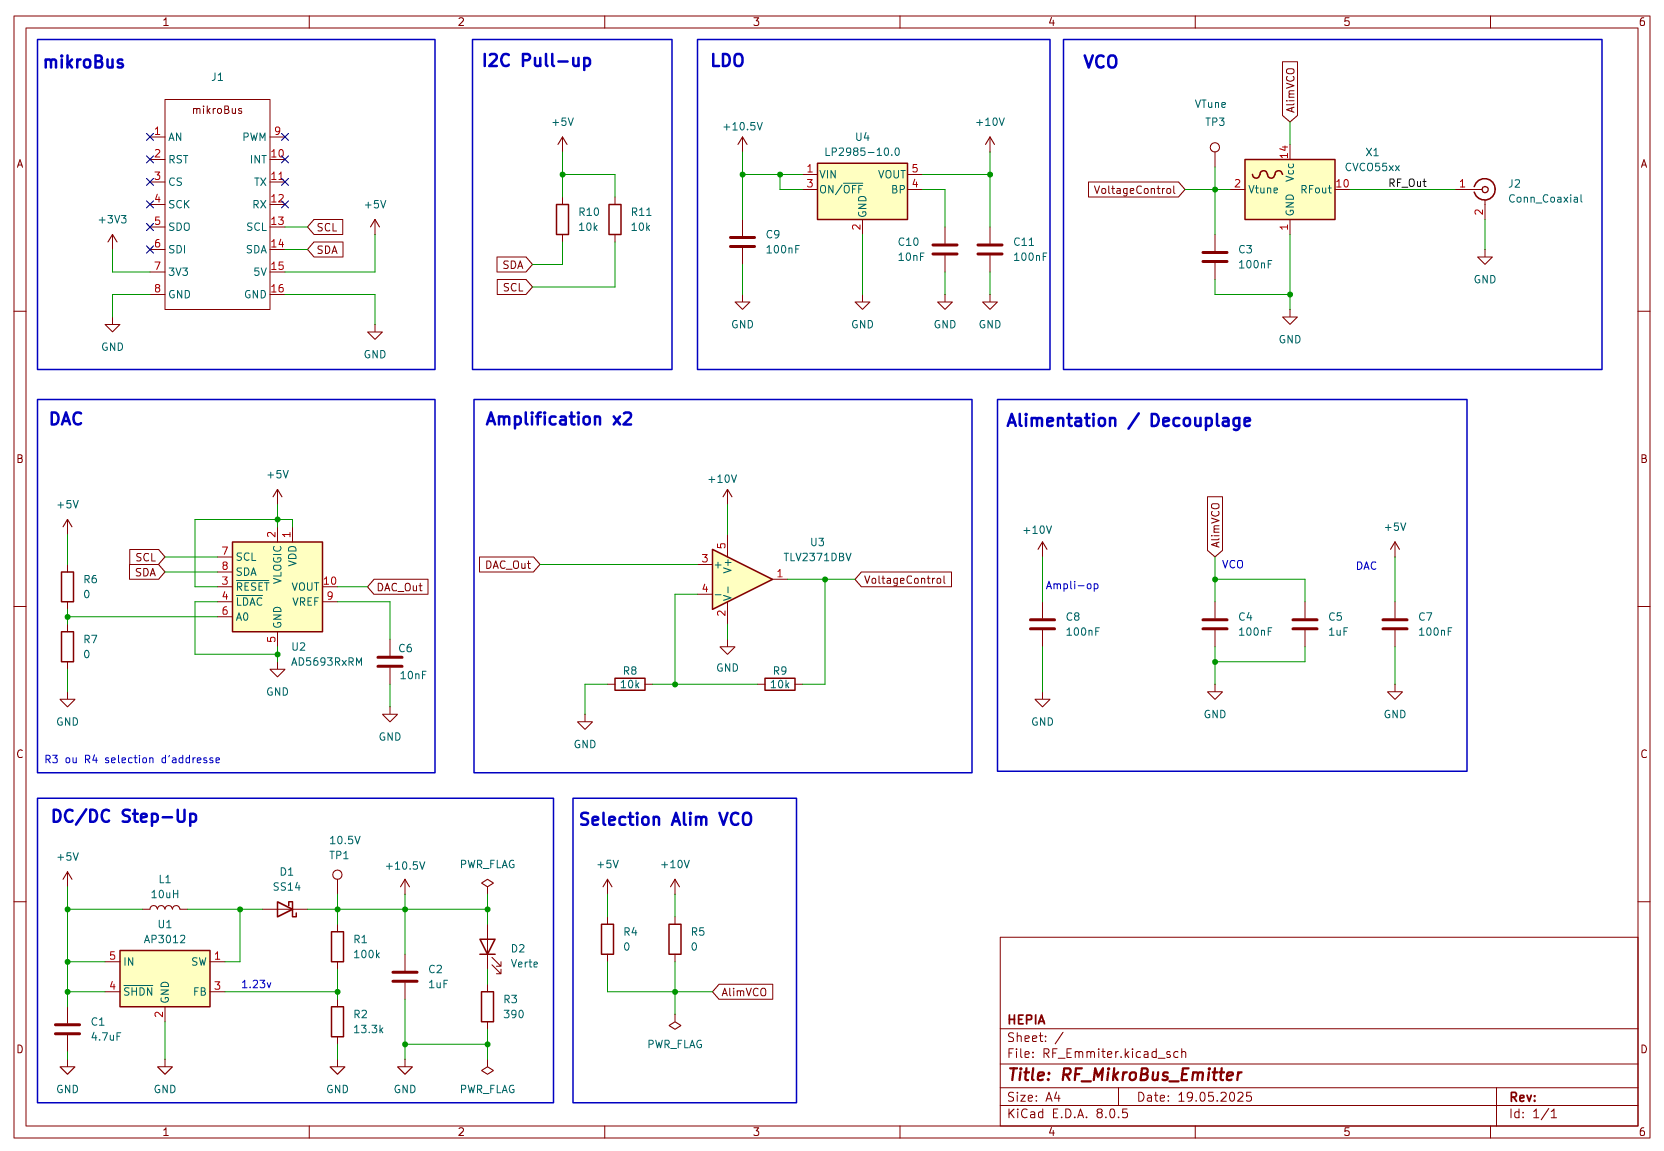
\includegraphics[scale=0.4, angle = 90]{images/rf_emit_sch.png}
    \caption{Schéma Émetteur RF}
    \label{fig:rf_emit_sch}
\end{figure}

\newpage
La \textbf{figure \ref{fig:rf_recv_sch}} est le schéma électrique du module mikroBus dre réception.
\begin{figure}[h]
    \centering
    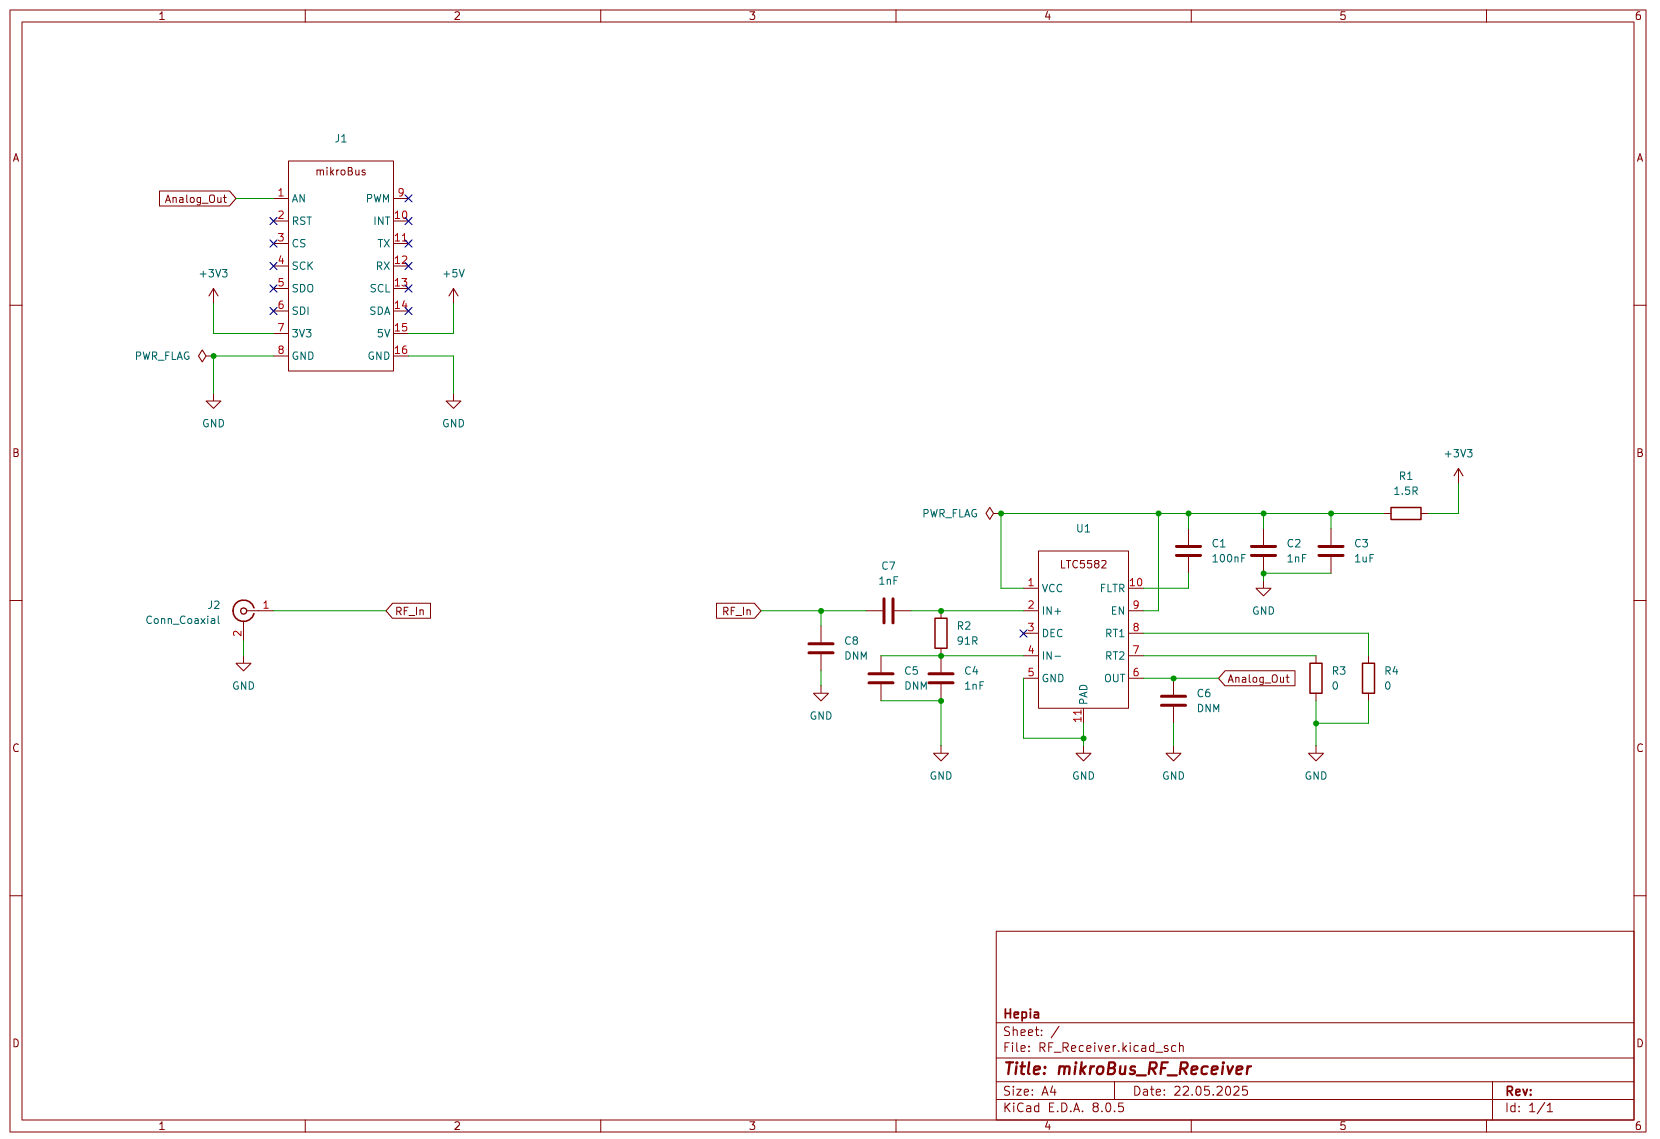
\includegraphics[scale=0.4, angle = 90]{images/rf_recv_sch.png}
    \caption{Schéma Récepteur RF}
    \label{fig:rf_recv_sch}
\end{figure}

\end{document}
